\documentclass[11pt,twoside]{article}

\usepackage{lgrind}
\usepackage{fullpage}
\usepackage{times}
\usepackage{doublespace}
\usepackage{epsfig}

%\title{Optimizing Stream Programs \\ Using a Linear State Space Representation}
%\title{A Linear State Space Representation \\ for Optimizing Stream Programs}
\title{~ \vspace{-48pt} \\ Optimizing Stream Programs \\ Using Linear State Space Analysis}

%% \author{Sitij Agrawal, William Thies, Rodric M. Rabbah, and Saman Amarasinghe \\
%%   MIT Computer Science and Artificial Intelligence Laboratory \\
%%   Cambridge, MA  02139\\ \\
%%   \sffamily{\{sitij, thies, rabbah, saman\}@csail.mit.edu}}

% don't include the date
\date{}

% this is the line spacing
\setstretch{1.9}

% \sloppy lets Latex be a little less anal about interword spacing.  It is
% one way to eliminate those annoying Overfull hbox warnings.
% Another way is to surround each offending paragraph with
% \begin{sloppypar} ... \end{sloppypar}

%\sloppy

% See page 90 of the Latex book for info about vertical spacing probs.

\begin{document}

  \newcommand{\subsubsubsection}[1]{\medskip\noindent{\bf #1}\\\smallskip}
  \newcommand{\mt}[1]{\mbox{\it #1}}
  \newcommand{\todo}[1]{\framebox{#1}}
  
  % shrink the itemized lists
  \newlength{\itemshrink}
  \setlength{\itemshrink}{-12pt}

  % shrink spacing of section titles
  \newcommand{\mysection}[1]{\vspace{-12pt} \section{#1} \vspace{-12pt}}
  \newcommand{\mysubsection}[1]{\vspace{-12pt} \subsection{#1} \vspace{-12pt}}
  \newcommand{\mysubsubsection}[1]{\vspace{-6pt} \subsubsection{#1} \vspace{-12pt}}

  % proper spacing of equations
  \newlength{\topeqn}
  \setlength{\topeqn}{-24pt}
  \newlength{\boteqn}
  \setlength{\boteqn}{-20pt}
  \newcommand{\starteqnstar}[0]{\begin{singlespace}\vspace{\topeqn}\begin{eqnarray*}}
  \newcommand{\doneeqnstar}[0]{\end{eqnarray*}\vspace{\boteqn}\end{singlespace}}
  \newcommand{\starteqn}[0]{\begin{singlespace}\begin{eqnarray}\vspace{\topeqn}}
  \newcommand{\doneeqn}[0]{\end{eqnarray}\vspace{\boteqn}\end{singlespace}}
  %\toappear{\centerline{\Large\bf MIT LCS Technical Memo,}
  %          \centerline{\Large\bf MIT-LCS-TM-6XX,}
  %          \centerline{\Large\bf November, 2001.}}
  
  \begin{singlespace}
    \maketitle
    \vspace{-48pt}
    \begin{abstract}
      Due to the high data rates involved in audio, video, and signal
processing applications, it is imperative to compress the data to
decrease the amount of storage used.  Unfortunately, this implies that
any program operating on the data needs to be wrapped by a
decompression and re-compression stage.  Re-compression can incur
significant computational overhead, while decompression swamps the
application with the original volume of data.

In this paper, we present a program transformation that greatly
accelerates the processing of compressible data.  Given a program that
operates on uncompressed data, we output an equivalent program that
operates directly on the compressed format.  Our transformation
applies to stream programs, a restricted but useful class of
applications with regular communication and computation patterns.  Our
formulation is based on LZ77, a lossless compression algorithm
utilized by ZIP, and immediately applies to simpler formats such as
Apple Animation, Microsoft RLE, and Targa.

We implemented a simple subset of our techniques in the StreamIt
compiler, which emits executable plugins for two popular video editing
tools: MEncoder and Blender.  For common operations such as color
adjustment and video compositing, computing directly on compressed
data offers a speedup roughly proportional to the overall compression
ratio.  For our benchmark suite of 12 videos in Apple Animation
format, speedups range from 1.1x to 471x, with a median of 15x.

    \end{abstract}
    \vspace{-12pt}
  \end{singlespace}
  
  \advance\topmargin by -0.35in      % Correct for LaTeX gratuitousness

  \section{Introduction}


Stream computing represents an increasingly important class of
applications. In streaming codes, there is an abundance of parallelism that
is easier to extract compared to traditional desktop workloads (e.g.,
pointer-based computing). As a result, the extraction of parallelism
in streaming codes does not require heroic efforts, and thus,
processors can deliver higher performance with significantly lower
power costs. This is especially important since
leading microprocessor companies have realized that modern general
purpose architectures are near their  performance limits for  the
amount of power they consume. Thus, the future will place a greater
emphasis on exploiting the properties of streaming workloads in
conventional von~Neumann architectures.

Streaming is a model of computation that uses sequences of data
and computation kernels to expose concurrency and locality for
efficiency~\cite{wss}. In general purpose processors, improving locality 
translates to an effective management of the memory hierarchy at all
levels, including the register file. In this paper, we present a
methodology for compiling streaming codes to general purpose,
cache-based architectures. We first introduce a simple model for
reasoning effectively about the caching behavior of streaming
workloads. This model serves as a foundation for several {\it cache-aware
optimizations} that are geared toward the concomitant increase of instruction
and data {\it temporal locality}. These
optimization lead to significantly better utilization of the memory
system, and as such, they deliver performance gains ranging from 11
to 99\% for our streaming benchmark suite.

The context for our work is StreamIt, an architecture-independent
language that is engineered for streaming
applications~\cite{streamitcc}. It adopts the 
Cyclo-Static Dataflow~\cite{BELP96} model of computation which is a
generalization of Synchronous Dataflow~\cite{LM87-i} (SDF).  
SDF is a popular  model that  is well suited for
streaming codes. In SDF, computation is represented as a graph
consisting of {\it  actors} connected by communication channels; the
actors consume  and produce a constant number  of items from their
input and output  channels every time they execute. SDF is appealing
because it is amenable to static scheduling and optimization. 

From a general purpose architecture's point of view, actors represent
computation kernels, and the communication between actors represents
data buffers that must be streamed to and from the processor. Thus
the size of an actor and the
order of actor executions are critical properties that
impact the performance of the instruction cache. For example, the
compiler must make sure the actor's code size is not
greater than the instruction cache. Furthermore, we must {\it scale}
the execution of the actor so that it runs several times before we move
on to some other actor in the stream 
graph. This serves to $(i)$ amortize the cost of fetching the actor's
instructions into the cache from memory (an expensive operation), $(ii)$
improve the instruction temporal locality, and $(iii)$ improve overall
performance. However, as our cache model will show, we 
cannot arbitrarily scale the execution frequency of an actor. This
is because actors produce data that must be buffered, and therefore,
we must also consider the amount of data an actor produces and
consumes if we are to adequately manage the data cache. This paper is unique
in that it is the first to present a unified optimization methodology
that simultaneously considers instruction and data locality for
mapping streaming computation to cache-based architectures.

In terms of improving the data cache behavior, the compiler schedules
actor firing such that the producer-consumer locality is
preserved. Furthermore,  the compiler may {\it fuse}
together two or more actors to form a coarser grained kernel.
The fusion allows for better register allocation as we can
destroy the arrays used to buffer data between the actors and replace
the corresponding array references with scalars.  It also allows for
various competing implementations for managing the buffers between the
fused actors.  This paper evaluates several implementation
alternatives (for buffer management) and evaluates their performance.

The methodology for fusing actors leverages a distinguishing StreamIt
characteristic, namely, the hierarchical organization of
the stream graph. Furthermore, the algorithm for fusing actors applies
for the various topologies allowed by StreamIt.
It also considers another distinguishing characteristics of StreamIt,
namely the {\tt peek} operation whereby an actor may inspect data
items in its input buffer without consuming them until some future
execution. While peeking is a powerful language feature, it does pose
some challenges to the compiler and the cache optimizations. Peeking
also impacts the choice for the best buffer management strategy, as our
study will show.

%% the comment about p3 and itanium not being embedded architectures
%% is out of the blue! need a better transition.
Cache-aware fusion alone delivers significant performance gains, although our
evaluation shows that fusion with scaling leads to the best
performance on a general purpose, cache-based architecture. For our
experiments, we use two different processors: a superscalar out-of-order
processor, and an in-order VLIW processor. The former is a Pentium~3
whereas the latter is an Itanium~2. While these architectures are not
particularly suited for an embedded system, they do exhibit some
properties that are worthy of investigation. Furthermore, that we can
demonstrate measurable performance gains on real systems is far more
convincing than using a simulation-based environment. We chose the
Pentium~3 processor because it has very few registers in its
instruction set architecture. The Itanium by contrast has a much 
larger and richer repertoire of registers. The two architectures serve
to validate our cache-aware optimizations, in that we expect an
architecture with more register to benefit more from optimization such
as scalar replacement. On average, fusion leads to a 47\% improvement
on the Pentium~3, and 50\% on the Itanium~2.

The two architectures also differ in terms of their memory system
organization. The Itanium is an in-order VLIW processor and does not
tolerate a memory stall as well as its out-of-order
counterpart. Therefore we expect different gains from the scaling
optimization which amortize the long access latencies for instruction
and data caches. On average, scaling leads to a 21\% improvement on
the Itanium~2, and 17\% on the Pentium~3.

While both scaling and fusion lead to modest performance gains, we
must combine the two to deliver the best possible performance. When we
do so, we can further improve the performance of our benchmarks by
53\% on average for the Pentium~3, and 55\% for the Itanium~2.

\subsection{Summary of Contributions}

This paper makes the following contributions:
\begin{itemize}

\item A cache model for stream computing that provides a quantitative
estimate of the caching performance for any sequence of actor
executions.

\item A cache-aware scheduling heuristic that judiciously increases
the multiplicity of actors, improving instruction and data locality
while not exceeding the data cache.

\item A cache-aware partitioning policy that judiciously fuses
adjacent actors into a single component, enabling local optimizations
while not exceeding the instruction cache.

\item An optimized buffer management policy, termed ``copy-shift with
execution scaling'', which out-performs a traditional rotating buffer
in a detailed micro-benchmark analysis.

\item A fully automatic implementation of the above techniques in the
StreamIt compiler.

\item An experimental evaluation across 11 streaming benchmarks,
demonstrating performance improvements of up to 99\%.
\end{itemize}

\subsection{Paper Roadmap}

The remainder of the paper is organized as follows. Section~\ref{sec:streamit}
describes StreamIt and introduces our motivating example.
Section~\ref{sec:cache-model} introduces our cache model for 
reasoning about the performance of a streaming
computation. Section~\ref{sec:cache-opt} describes our cache-aware
optimizations, and Section~\ref{sec:buffer} describes the 
optimization enabled by fusion. Section~\ref{sec:evaluation} describes
our evaluation methodology and present our experimental
analysis. Sections~\ref{sec:related-work}~and~\ref{sec:conclusion}
discuss related work and concludes the paper.

  \mysubsection{The StreamIt Language}
\label{sec:background}

StreamIt~\cite{streamitcc} is an architecture-independent language for
signal processing applications.  StreamIt aims to expose the abundant
parallelism and regular communication patterns in stream programs for
the benefit of the compiler.  The optimizations described in this
paper would be infeasible in a general-purpose language such as C.  As
detailed elsewhere~\cite{streamitcc}, C obscures the high-level
structure of a streaming application due to possible aliasing between
autonomous filters, complex modulo expressions on circular buffers,
and muddling of atomic execution steps with global control flow.
%There is not enough information in C code to automatically perform the
%high-level transformations that experts use to achieve competitive
%performance.  
In addition, StreamIt offers improved programmer productivity over C
due to its parameterizable and composable stream constructs.

The basic programmable unit in StreamIt is a filter; for example, see
the {\tt MovingAverage} filter in Figure~\ref{fig:filter-example}.  A
filter contains a work function which executes atomically, popping a
fixed number of items from the filter's input tape and pushing a fixed
number of items to the filter's output tape.  A filter can also
``peek'' at a given index on its input tape without consuming the
item; this makes it simple to write sliding-window applications such
as the {\tt MovingAverage}.  The push, pop, and peek rates are
declared on the same line as the work function, thereby enabling the
compiler to construct a static schedule of filter
firings~\cite{lee87static}.

Each filter has a distinct address space.  A filter can store two
types of variables: a {\it field} and a {\it local}.  Fields are
declared in the scope of the filter and are preserved across
executions, while locals are declared inside the work function and are
only live within a single execution.  There is also an init function,
run once at the beginning of the program, that can be used to
initialize fields.

StreamIt provides three hierarchical structures for composing filters
into larger stream graphs (see Figure~\ref{fig:structures}).  The {\it
pipeline} construct composes streams in sequence, with the output of
one connected to the input of the next.  The {\it splitjoin} construct
distributes data to a set of parallel streams, which are then joined
together in a roundrobin fashion.  The {\it feedback loop} provides a
mechanism for introducing cycles in the graph.  An example of a
pipeline appears in Figure~\ref{fig:iir-pipeline}.  It contains a
single IIR (Infinite Impulse Response) filter, which could be
implemented as shown at the top of Figure~\ref{fig:opt-seq}.

\begin{figure}[t]
\begin{minipage}{3.25in}
{\scriptsize
\begin{verbatim}
float->float filter MovingAverage(int N) {
  float[N] weights;  // a filter field

  // init function initializes the weights
  init {
    for (int i=0; i<N; i++)
      weights[i] = 1/N;
  }

  // work func. declares push, pop, peek rates
  work push 1 pop 1 peek N {
    float result = 0;  // a local variable
    for (int i=0; i<N; i++) {
      result += weights[i] * peek(i);
    }
    push(result);
    pop();
  }
}         
\end{verbatim}
\vspace{-18pt}
\caption{Example of a StreamIt filter.~~~~~~~\protect\label{fig:filter-example}}}
\end{minipage}
\vrule
\begin{minipage}{3.50in}
\begin{singlespace}

~~~~
\hspace{0.1in}\begin{minipage}{0.46in}
{\centering
\psfig{figure=pipeline.eps,width=0.46in} \\
}
\end{minipage} 
~
\begin{minipage}{1.3in}
{\centering
\psfig{figure=splitjoin.eps,width=1.3in} \\
}
\end{minipage}
~
\begin{minipage}{1.02in}
{\centering
\psfig{figure=feedback.eps,width=1.02in} \\
}
\end{minipage}

%\\ ~ \\ {\protect\small \mbox{~}(a) A pipeline. ~~~~~~~~~~(b) A splitjoin. ~~~~~~~~~~~~~~(c) A feedbackloop.}
~ \vspace{-6pt} \\ {\protect\footnotesize \mbox{~~~~}\hspace{0.1in}(a) pipeline ~~~~~~~~~(b) splitjoin ~~~~~~~~~~~~(c) feedbackloop}
\vspace{-6pt}
\caption{Structures supported by StreamIt.
\protect\label{fig:structures}}
\vspace{8pt}
\hrule
~~\hspace{0.2in}\begin{minipage}{3in}
\vspace{8pt}
\psfig{figure=iir-pipeline.eps, width=2.33in}
~~~~
\raisebox{12pt}{\psfig{figure=iir-pipeline2.eps, width=0.46in}}

~ \\ \vspace{-49.5pt}
\caption{Example pipeline with IIR filter.~~\protect\label{fig:iir-pipeline}}
\end{minipage}
\vspace{6pt}
%\vspace{6pt}
\end{singlespace}
\end{minipage}
\hrule
\end{figure}

%%         A filter can store two types of variables - \textit{field} and
%% \textit{local}. Field variables are declared outside of the
%% specific functions (work, prework, init), and can be accessed from
%% anywhere within the filter. Local variables are declared within a
%% specific function, and only have scope within that function. For
%% example, a variable declared within the init function is local,
%% and could not be accessed within the work function. Therefore, the
%% init function is used to initialize field variables.

\mysubsection{State Space Example}

As described previously, a linear state space model describes a stream
in which both the outputs and the state values are updated as a linear
combination of the inputs and the previous states.  We use the
following notation to describe such systems:

\hspace{0.5in}\begin{minipage}{2.5in}
\starteqnstar 
\vc{\dot{\mathbf{x}}} & = & \mathbf{A}\vc{\mathbf{x}} +
\mathbf{B}\vc{\mathbf{u}} \
\doneeqnstar
\end{minipage}
\begin{minipage}{2.5in}
\starteqnstar 
\vc{\mathbf{y}}
& = & \mathbf{C}\vc{\mathbf{x}} + \mathbf{D}\vc{\mathbf{u}}
\doneeqnstar
\end{minipage}

\noindent In these equations, the state vector is denoted by
$\vc{\mathbf{x}}$, the inputs by $\vc{\mathbf{u}}$, and the outputs
by $\vc{\mathbf{y}}$. $\vc{\dot{\mathbf{x}}}$ represents the new
state vector, i.e., the state vector after it is updated. The first
equation is for the state updates, while the second equation is for the
outputs.  $\mathbf{A}$, $\mathbf{B}$, $\mathbf{C}$, and
$\mathbf{D}$ are matrices whose dimensions depend on the number of
states, inputs, and outputs.

Figure~\ref{fig:opt-seq} illustrates an optimization sequence for an
IIR filter.  Three versions of the filter are shown: original,
following state removal, and following parameter reduction.  In each
case, the state space representation for the filter is shown on the
right, along with the number of multiplications and additions needed
per execution of the work function.

The state removal optimization identifies that the states $x_1$ and
$x_2$ are always used as part of the expression $x_1 + x_2$.  Thus,
one of the states can be eliminated in favor of a single variable,
$x$, that tracks the value of the sum.  While relatively simple in
this example, such a transformation can be quite subtle when applied
to a large representation (e.g., the result of combining many filters
together.)  State removal can reduce storage requirements as well as
eliminate arithmetic operations (in this example, 1 multiplication and
4 additions).  As described in Section~\ref{sec:state-removal}, state
removal is formulated as a general sequence of matrix operations.

The parameter reduction optimization refactors the coefficients that
operate on the state variables in order to reduce the number of
operations needed.  Following the transformation, $x$ assumes a value
that is twice as large as the original (at any given point of
execution).  However, this change does not affect the output of the
filter, as the coefficients in $\mathbf{A}$ are compensated
accordingly.  The transformation enables two coefficients in
$\mathbf{B}$ and $\mathbf{C}$ to change to a value of 1, thereby
eliminating two multiplication operations.  As described in
Section~\ref{sec:parameter-reduction}, this transformation is also
formulated as a general series of matrix operations.

%%     StreamIt is a programming language specifically tailored to DSP
%% streaming applications. The user creates a graph composed of four
%% types of StreamIt constructs: \textit{filters},
%% \textit{pipelines}, \textit{splitjoins}, and \textit{feedback
%% loops}. Filters encapsulate the computation done within an
%% application - they represent the blocks mentioned in the previous
%% section. Each filter operates on a one-dimensional `tape' of
%% values (of any type, including structures and arrays).  The other
%% three constructs dictate the type of connections possible between
%% filters. Every construct explicitly states its input type and
%% output type, and can be passed parameters as would be to a
%% procedure.

%%     StreamIt uses a buffer between every pair of filters to
%% hold values. When the input buffer of a construct (equivalent to
%% the output buffer of the previous construct) is appropriately
%% filled, the construct can execute. Execution involves three steps:
%% reading and removing items from the input buffer (consumption);
%% performing computations; putting items in the output buffer
%% (production). We will not consider the intricacies of managing
%% these buffers, and instead refer to the more abstract notion of a
%% tape.

%%     A filter has pre-defined \textit{peek}, \textit{pop}, and
%% \textit{push} rates (StreamIt code examples are given below).
%% During each execution, the filter accesses a maximum of peek
%% values from its input tape, consumes exactly pop input values from
%% its input tape, and produces exactly push values onto its output
%% tape. Since the removal of an input value is technically an access
%% of that input, the peek rate of a filter must be greater than or
%% equal to the pop rate of that filter. The push or pop rate can be
%% zero - the former corresponds to a filter that consumes items but
%% does not produce them (typically the last filter in a sequence)
%% and the latter corresponds to a filter that produces items but
%% does not consume them (typically the first filter in a sequence).
%% All the accesses, outputs, and removals, as well as all the
%% computation is done inside the main body of the filter, known as
%% the work function.

%% \begin{figure}[bthp]
%%   \centering
%%   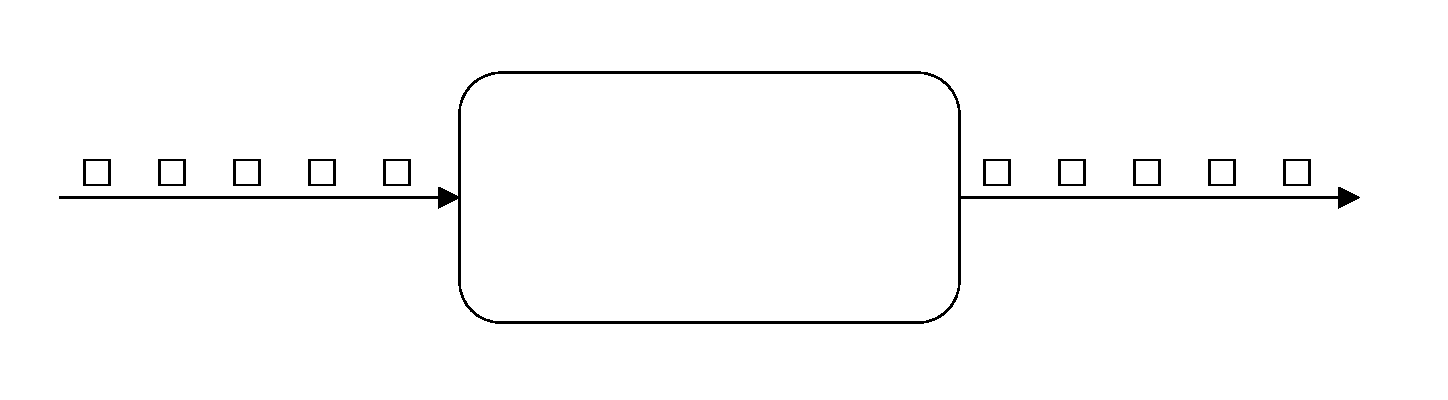
\includegraphics[width=3.0in]{figures/filter.eps}
%%   \caption{StreamIt filter}
%%   \label{fig:filter}
%% \end{figure}

%%     StreamIt also supports a \textit{prework} function, which has its own push,
%% pop, and peek rates.  The prework function executes in place of
%% the work function for the first computation sequence, and is never
%% run again. Additionally, there is an \textit{init} function which
%% is run only once upon creation of the filter, and is usually used
%% to initialize variables.  The init and prework functions are both
%% optional.

%%         A filter can store two types of variables - \textit{field} and
%% \textit{local}. Field variables are declared outside of the
%% specific functions (work, prework, init), and can be accessed from
%% anywhere within the filter. Local variables are declared within a
%% specific function, and only have scope within that function. For
%% example, a variable declared within the init function is local,
%% and could not be accessed within the work function. Therefore, the
%% init function is used to initialize field variables.

%% Code examples of StreamIt filters are shown below.

%% \begin{scriptsize}
%% \begin{singlespace}
%% \begin{verbatim}
%% // This filter adds the parameter scalar to each input.
%% // It does not have an init or prework function
%% float -> float filter scalarAdd(float scalar) {
%%   work push 1 pop 1 peek 1 {
%%     push(scalar + pop());
%%   }
%% }
%% \end{verbatim}
%% \end{singlespace}
%% \end{scriptsize}

%% \begin{scriptsize}
%% \begin{singlespace}
%% \begin{verbatim}
%% // This filter outputs a running average of every three consecutive inputs.
%% // The first time it runs, it ouputs the average of the first two inputs without removing anything from the tape.
%% // It does not have an init function.
%% float -> float filter threeWayAverage() {
%%   prework push 1 pop 0 peek 2 {
%%     float temp;  // example of a local variable
%%     temp = (peek(0)+peek(1))/2;
%%     push(temp);
%%   }
%%   work push 1 pop 1 peek 3 {
%%     float temp;  // example of a local variable
%%     temp = (peek(0) + peek(1) + peek(2))/3
%%     push(temp);
%%     pop()
%%   }
%% }
%% \end{verbatim}
%% \end{singlespace}
%% \end{scriptsize}

%% \begin{scriptsize}
%% \begin{singlespace}
%% \begin{verbatim}
%% // This filter computes an infinite impulse response function.
%% // It does not have a prework function.
%% float->float filter IIR() {
%%     float curr;  // example of a field variable
%%     init {
%%       curr = 0;
%%     }
%%     work push 1 pop 1 peek 3 {
%%       float temp;  \\ example of a local variable
%%       temp = (peek(0) + peek(1) + peek(2))/6;
%%       curr = temp + curr/2;
%%       push(curr);
%%       pop();
%%     }
%% }
%% \end{verbatim}
%% \end{singlespace}
%% \end{scriptsize}

%%     Pipelines, splitjoins, and feedback loops are higher level
%% constructs created from filters. Each structures the layout of its
%% filters in a certain format. Even though these three constructs do
%% not directly provide the syntax to perform computations and work
%% from an input or output tape, they can be thought of as filters in
%% the following way: the construct recieves inputs which are passed
%% to one or more of the filters; all the filters perform
%% computations and pass values to one another through their input
%% and output tapes; the construct outputs values from one or more of
%% its filters. In fact, for every pipeline, splitjoin, and feedback
%% loop there is an equivalent filter representation. Therefore,
%% these three constructs are not strictly necessary for writing a
%% StreamIt program. However, they simplify and structure writing a
%% large application.

%%     The higher level constructs are not limited to combine filters -
%% they can also combine each other. This follows directly from the
%% fact that a higher level construct has some equivalent filter.
%% Therefore, if a pipeline can be composed of filters, it can also
%% be composed of pipelines, splitjoins, and feedback loops, which
%% are all like filters. We shall refer to all four StreamIt
%% constructs generically as blocks. This corresponds to the fact
%% that any StreamIt construct behaves as a block: it takes inputs,
%% performs calculations, and produces outputs.

%%     Pipelines combine a set of blocks in sequential fashion, so that
%% the output of the first block is the input to the second block,
%% the output of the second block is the input to the third block,
%% etc. The blocks are placed in order using the add statement.

%% \begin{figure}[bthp]
%%   \centering
%%   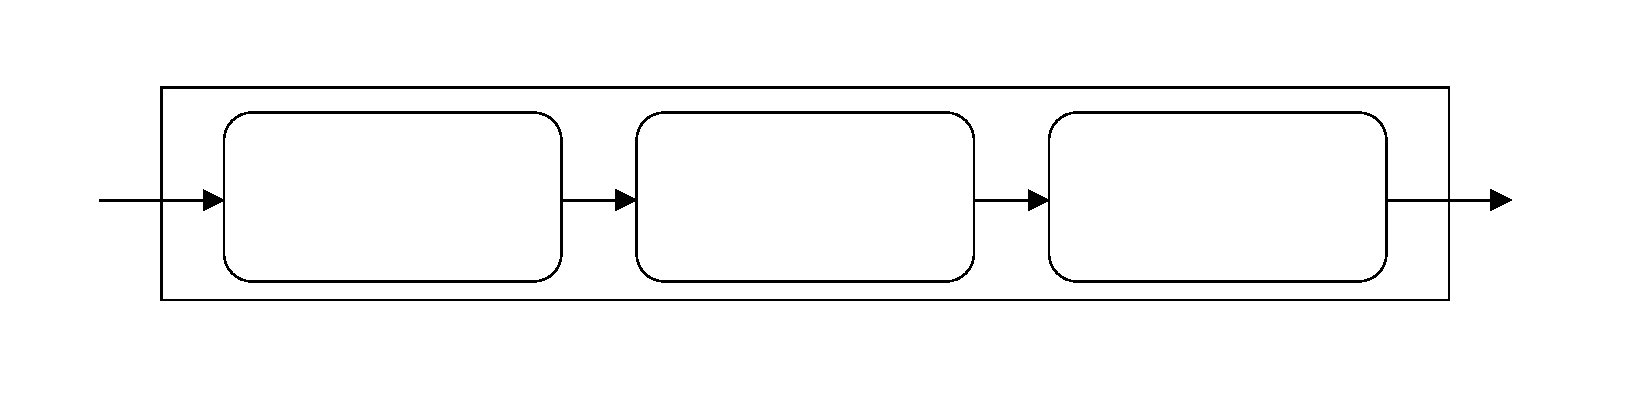
\includegraphics[width=3.0in]{figures/pipeline.eps}
%%   \caption{StreamIt pipeline}
%%   \label{fig:pipeline}
%% \end{figure}

%% \begin{scriptsize}
%% \begin{singlespace}
%% \begin{verbatim}
%% // This pipeline connects the filters scalarAdd and threeWayAverage.
%% // The parameter scalar passed to this pipeline is passed to the
%% // filter scalarAdd.
%% float -> float pipeline combinedWork(float scalar) {
%%   add scalarAdd(scalar);
%%   add threeWayAverage();
%% }
%% \end{verbatim}
%% \end{singlespace}
%% \end{scriptsize}

%%     A splitjoin arranges blocks in a parallel fashion.  The inputs to
%% a splitjoin are sent to each block in a \textit{roundrobin} or
%% \textit{duplicate} manner, and the outputs of each block are
%% joined in a roundrobin manner. Duplicate splitting means the
%% inputs to the splitjoin are copied and sent to each block, so that
%% each block receives exactly the same set of inputs.  Roundrobin
%% splitting means the inputs to the splitjoin are sent to each block
%% according to user defined weights.  For example, the first block
%% receives two inputs, the second block receives one input, the
%% third block receives two inputs.  Therefore, each block sees a
%% different set of inputs. Roundrobin joining (the only type of
%% joining permitted) means the outputs of each block are combined
%% according to user defined weights, and these represent the outputs
%% of the entire splitjoin. Blocks are listed in the order which they
%% recieve inputs using add statements. The way inputs are sent is
%% determined by using the split statement before the block list, and
%% the way outputs are recieved is determined by using the join
%% statement after the block list.

%% \begin{figure}[bthp]
%%   \centering
%%   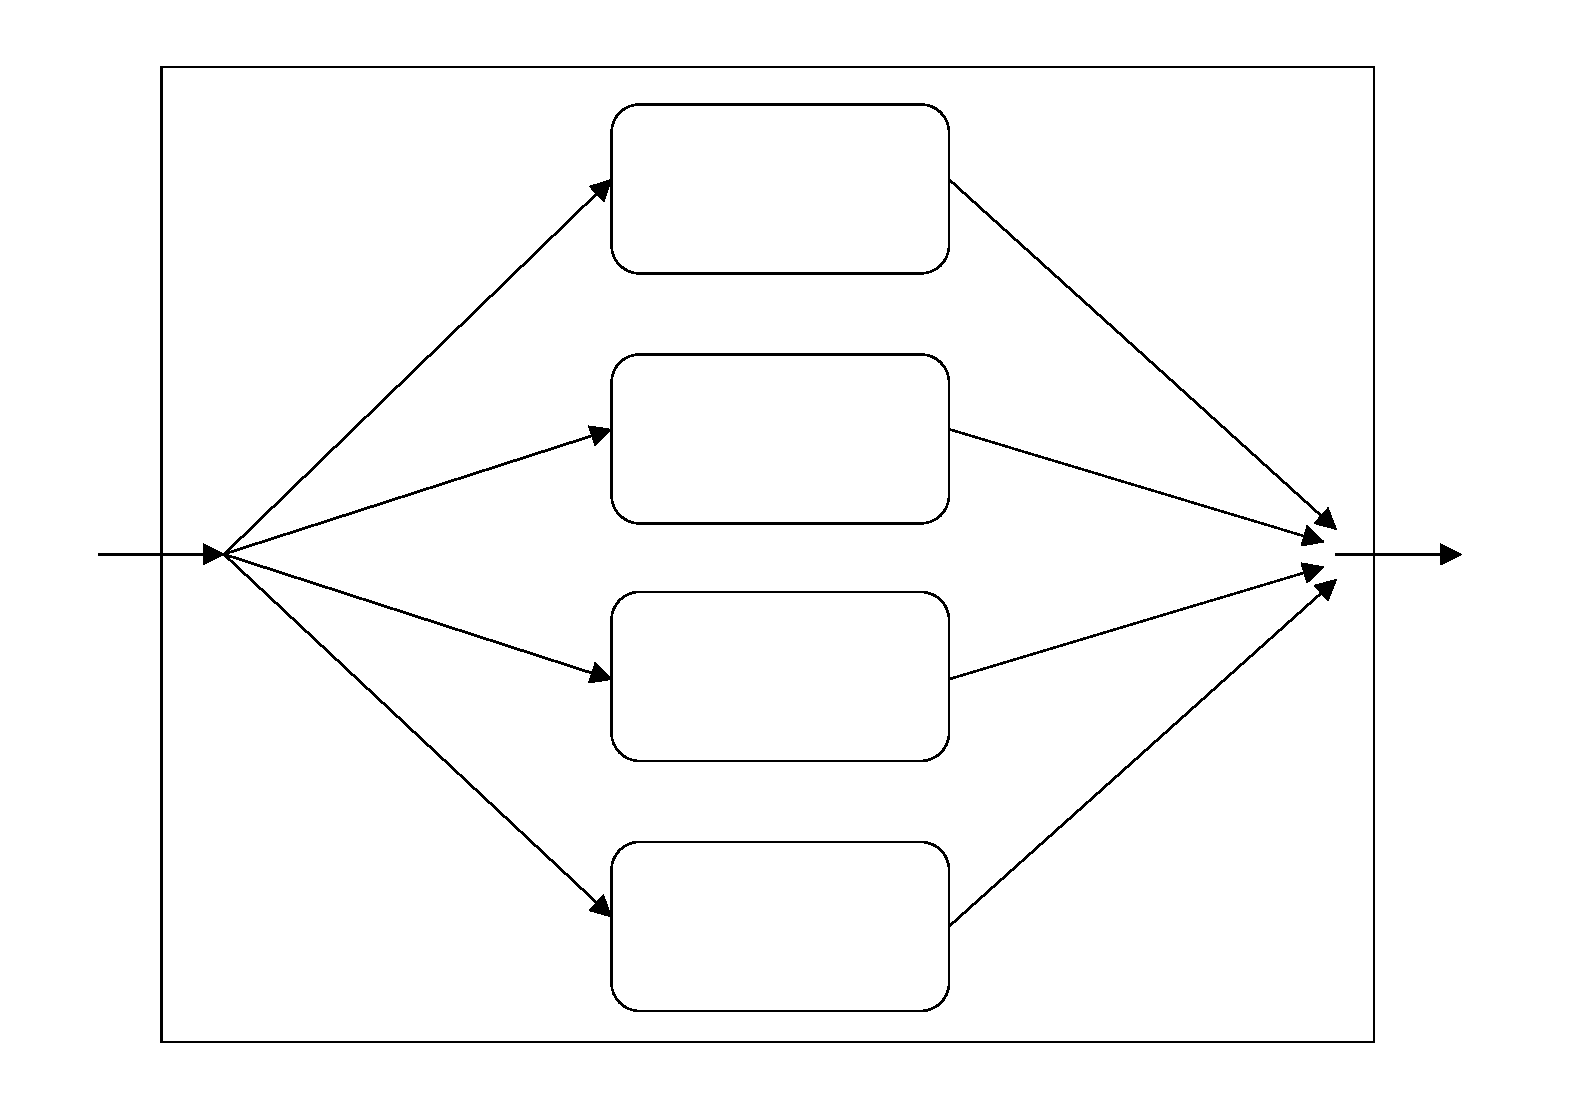
\includegraphics[width=3.0in]{figures/splitjoin.eps}
%%   \caption{StreamIt splitjoin}
%%   \label{fig:splitjoin}
%% \end{figure}

%% \begin{scriptsize}
%% \begin{singlespace}
%% \begin{verbatim}
%% // This splitjoin splits its inputs three ways.
%% // The first two inputs are sent to the first block, the next
%% // input to the second block, and the next two inputs to the third
%% // block.
%% // The outputs are collected in the following manner: three from
%% //the first block, five from the second block, and four from the
%% // third block.
%% // For every 2+1+2=5 values inputted, 3+5+4=12 values are
%% // outputted.
%% float -> float splitjoin mySplitjoin() {
%%  split roundrobin(2,1,2);
%%   add combinedWork(3.5);
%%   add combinedWork(4.5);
%%   add threeWayAverage();
%% join roundrobin(3,5,4);
%% }
%% \end{verbatim}
%% \end{singlespace}
%% \end{scriptsize}

%%     A feedback loop uses some of its output as
%% an input. It consists of a body block and a loop block. The input
%% to the entire feedback loop is combined with the output of the
%% loop block and sent to the body block, via a roundrobin joiner.
%% The output of the body block is split two ways in a roundrobin or
%% duplicate manner.  The first set of outputs is used as the output
%% of the entire feedback loop, and the second set of outputs is used
%% as the input to the loop block. Note that there must be initial
%% values enqueued on the output tape of the loop block in order for
%% the feedback loop to begin executing. The first statement in a
%% feedback loop is a join, determining how inputs are sent to the
%% body block. The body and loop blocks are listed next. The last
%% statement is a split, determining where outputs are sent from the
%% loop block.

%% \begin{figure}[bthp]
%%   \centering
%%   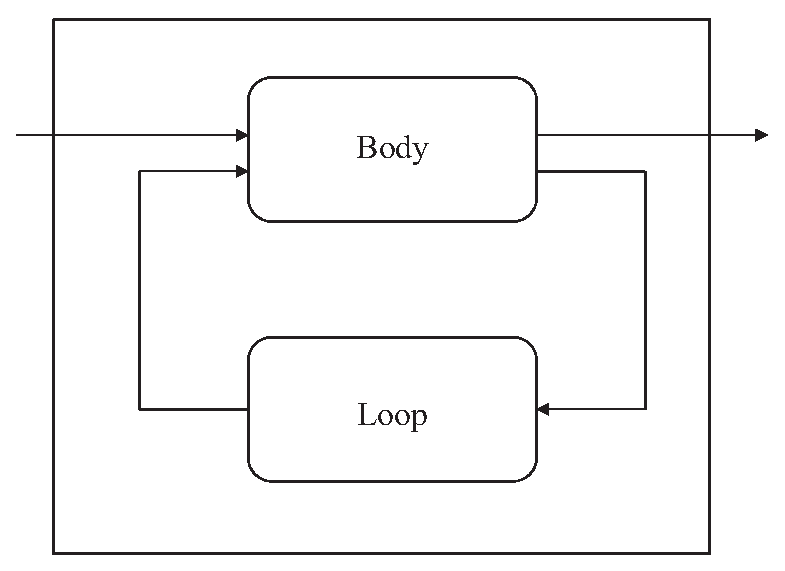
\includegraphics[width=3.0in]{figures/feedback.eps}
%%   \caption{StreamIt feedback loop}
%%   \label{fig:feedback}
%% \end{figure}

%% \begin{scriptsize}
%% \begin{singlespace}
%% \begin{verbatim}
%% // This is a feedback loop implementation of the IIR filter.
%% // The body and loop are both anonymous filters.
%% float -> float feedbackloop IIRFeedback() {
%%   join roundrobin(3,1);
%%   body float->float filter {
%%     work push 1 pop 1 peek 4 {
%%       push((peek(0)+peek(1)+peek(2))/6 + peek(3)/2);
%%       pop();
%%     }
%%   };
%%   loop float->float filter {
%%     work push 1 pop 1 peek 1 {
%%       push(pop());
%%     }
%%   };
%%   split duplicate();
%%   enqueue(0.0);
%% }
%% \end{verbatim}
%% \end{singlespace}
%% \end{scriptsize}

%%     To run a program, the StreamIt compiler finds a
%% steady-state schedule of the number of times to execute each
%% filter \cite{Karczmarek}. If such a schedule cannot be found, the
%% user created block diagram is ill-formed and could not represent a
%% real world application.

%% \mysubsection{Block Representations}

%%     The execution of a block (StreamIt or otherwise) can by
%% characterized by a single equation if the block is linear, and a
%% pair of equations if the block is state space linear. We describe
%% these terms in detail below.

%% \mysubsubsection{Linear Representations}

%%     A block is termed linear if its outputs are a linear
%% combination of its inputs plus a set of constants. In mathematical
%% terms, this relationship can be modelled by the equation
%% $\vc{\mathbf{y}} = \mathbf{D}\vc{\mathbf{u}} +
%% \vc{\mathbf{b}}$, where $\vc{\mathbf{u}}$ is a column vector
%% representing the inputs, $\mathbf{D}$ is a matrix representing the
%% weights applied to each input, $\vc{\mathbf{b}}$ is a column
%% vector representing constants added to the inputs, and
%% $\vc{\mathbf{y}}$ is a column vector representing the outputs.

%%     Suppose we have the following linear model:
%% \starteqnstar
%% \vc{\mathbf{y}} = \left [ \begin{array} {cc} 1 & 2 \\ 3 & 4 \\
%% 5 & 6 \end{array} \right ] \vc{\mathbf{u}} + \left [
%% \begin{array} {c} 7
%% \\ 8 \\ 9 \end{array}\right ]
%% \doneeqnstar

%%     It is exactly described by the following StreamIt filter:
%% \begin{scriptsize}
%% \begin{singlespace}
%% \begin{verbatim}
%% int -> int filter linearFilter() {
%%   work push 3 pop 2 peek 2 {
%%     push(1*peek(0) + 2*peek(1) + 7);
%%     push(3*peek(0) + 4*peek(1) + 8);
%%     push(5*peek(0) + 6*peek(1) + 9);
%%     pop(); pop();
%%   }
%% }
%% \end{verbatim}
%% \end{singlespace}
%% \end{scriptsize}

%%     A process for analyzing and optimizing linear StreamIt filters
%% is described in \cite{Lamb}.

  \section{State-Space Analysis}

  We analyze StreamIt programs at the filter level. We create
a data structure representation that fully describes a state-space
filter. We parse the code of each StreamIt filter to determine
whether or not it is state-space; if so we initialize a data
structure, fill it with the appropriate values through a process
called \emph{extraction}, and associate the structure with the
filter.

    We provide a set of rules to combine state-space representations
of filters in higher StreamIt blocks---pipelines, splitjoins, and
feedback loops. Such a process results in a single state-space
representation for the entire block. Some representations may need
to change so that they are properly combined. We detail what the
changes are and when they need to be made. Finally, we describe
how to convert a representation back to StreamIt code for a
filter.

\subsection{Representation}

    Our first task is to create a data structure that fully captures
the state-space representation of a StreamIt filter.  We save a
filter's number of states, push rate, and pop rate in variables
which we term $s$, $u$, and $o$, respectively. Our data structure
also contains the matrices $\mathbf{A}$, $\mathbf{B}$,
$\mathbf{C}$, and $\mathbf{D}$ with dimensions $s \times s$, $s
\times o$, $u \times s$, and $u \times o$, respectively. The
inputs to a filter are denoted as $\vec{\mathbf{u}}$ (length $o$),
the outputs as $\vec{\mathbf{y}}$ (length $u$), and the states as
$\vec{\mathbf{x}}$ (length $s$). Upon every execution of the
filter, we can calculate the outputs by the formula
$\vec{\mathbf{y}} = \mathbf{C}\vec{\mathbf{x}} +
\mathbf{D}\vec{\mathbf{u}}$, and update the state matrix by the
formula $\vec{\dot{\mathbf{x}}} = \mathbf{A}\vec{\mathbf{x}} +
\mathbf{B}\vec{\mathbf{u}}$. For convenience, we will calculate
the filter outputs before updating the state matrix. Since the
states may have initial values other than zero, we store these
values as the vector $\overrightarrow{\mathbf{initVec}}$ (length
$s$).

    Since we have not included a constant term in our model, we
will set one of the state variables to be the constant $1$. This
variable will not be updated by any of the states or inputs, and
its initial value will be $1$, so it will always remain that
value. Any state or output that depends on a constant term can now
refer to a multiple of the constant state variable instead.

    As long as a filter's peek rate (which we term $e$) equals its pop
rate, the data structure as currently designed can fully represent
the filter. We must include additional modifications for a filter
with a peek rate greater than its pop rate. Note that such a
filter still removes $o$ items from its input tape upon every
execution, but it accesses $e-o$ additional items on its input
tape. Therefore, our current data structure would work as long as
there is some way to access these additional items.

    We solve the problem of having a peek rate greater than a pop
rate by storing $e-o$ items from the input tape in the state
vector $\vec{\mathbf{x}}$. Therefore, when a filter executes, it
can access all $e$ items it needs, $o$ items from its input vector
and $e-o$ items from its state vector. These $e-o$ states must be
updated by the inputs and themselves - the specifics are covered
in the next section. We store the number of states used for inputs
as the variable $stored$. This will be useful when combining
representations.

    When the filter is executed for the first time, it will have access
to the $o$ items in the input vector, but the $e-o$ states it
needs will be uninitialized from the input tape. Therefore, we
need to update the state vector before computing the output/state
update equation pair for every filter execution. We introduce two
new matrices, $\mathbf{A_{pre}}$ and $\mathbf{B_{pre}}$ to perform
this initialization. Before the filter runs it will perform the
state update $\vec{\dot{\mathbf{x}}} =
\mathbf{A_{pre}}\vec{\mathbf{x}} +
\mathbf{B_{pre}}\vec{\mathbf{u_{pre}}}$. The initialization input
vector, $\vec{\mathbf{u_{pre}}}$, has length $o_{pre} = e-o$. For
now, $o_{pre}$ and $stored$ have the same value, but combining
filters might result in $o_{pre}$ being greater than $stored$.
$\mathbf{A_{pre}}$ is $s \times s$ and $\mathbf{B_{pre}}$ is $s
\times o_{pre}$. Note that initial assignments of the state
variables by $\overrightarrow{\mathbf{initVec}}$ are done
immediately when a filter is created, while initialization by
$\mathbf{A_{pre}}$ and $\mathbf{B_{pre}}$ is afterwards, when
there are a sufficient number ($o_{pre}$) of items on the input
tape.

    Putting these pieces together, we find a full representation
consists of the push and pop rates, the number of state variables,
the number of stored inputs, the four state matrices, an initial
state vector, and possibly an initial pop rate and two
initialization state matrices. We define a state-space
representation $\mathrm{R}$ as the tuple $\langle$$u$, $o$, $s$,
$stored$, $\mathbf{A}$, $\mathbf{B}$, $\mathbf{C}$, $\mathbf{D}$,
$\overrightarrow{\mathbf{initVec}}$, $\mathbf{A_{pre}}$,
$\mathbf{B_{pre}}$, $o_{pre}$$\rangle$. When we introduce a
representation $\mathrm{R_i}$, each of its values in the ordered
set will be denoted with the index $i$ (for example $u_i$,
$\mathbf{A_i}$). For representations of filters that do not need
the initialization matrices, we will write $\mathbf{A_{pre}} =
null$, $\mathbf{B_{pre}} = null$, $o_{pre} = 0$. In this case, the
filter will not have any stored inputs, so $stored = 0$ as well.

    Representations are initially created from StreamIt filters and
ultimately converted to StreamIt filters. Between these steps,
however, representations of the higher StreamIt block types can be
derived by combining the representations of their parts.
Therefore, from now on we will say that a representation refers to
a block rather than a filter. The exception is in Section 3.2,
where we discuss how to create a representation from a StreamIt
filter. Hence we explicitly refer to a filter rather than block
representation in that section.

\subsection{Extraction}

    We write a module that extracts the state-space representation of
a filter. We symbolically execute a single iteration of a filter's
work function, maintaining a vector pair representation for each
local variable and filter field variable that is encountered
(combined, these are termed program variables). If the outputs and
field variables all have vector pair representations, then the
filter is state-space linear, and the vectors are used as rows of
$\mathbf{A}$, $\mathbf{B}$, $\mathbf{C}$, and $\mathbf{D}$. This
type of procedure is termed data flow analysis. See \cite{Lamb}
for a treatment of the linear case.

    We attempt to find a vector pair
($\vec{\mathbf{v}}$,$\vec{\mathbf{w}}$) for each program variable
$y$ where $y = \vec{\mathbf{v}} \cdot \vec{\mathbf{u}} +
\vec{\mathbf{w}} \cdot \vec{\mathbf{x}}$. $\vec{\mathbf{u}}$ is
the filter input vector and $\vec{\mathbf{x}}$ is the filter state
vector. When $y$ is on the left hand side of an assignment
statement, terms from the right hand side are compared with
entries from $\vec{\mathbf{u}}$ (inputs) and $\vec{\mathbf{x}}$
(states). The coefficients from terms that match are used for to
fill the corresponding entries in $\vec{\mathbf{v}}$ and
$\vec{\mathbf{w}}$, as long as they are constants. If any
coefficient is not a constant, then $y$ is non-linear.

    The input vector, $\vec{\mathbf{u}}$, is defined as $[peek(e-o)
~peek(e-o+1) ~... ~peek(o-1)]$. The state vector,
$\vec{\mathbf{x}}$, holds $e-o$ variables from the input tape
($peek(0) ~... ~peek(e-o-1)$), every field variable, and a
variable for the constant 1. We do not consider local variables
for the state vector, because their values are not saved across
filter executions. Therefore, their values should be resolved to
constants at compile time. A field variable has the initial vector
pair ($\vec{\mathbf{0}}$,$\left [
\begin{array} {ccccc} 0 & ... & 1 & ... & 0 \end{array} \right
]$), where the 1 corresponds to the field variable itself.

    If the vector pair can be found, then the program variable $y$ can
be written as a linear combination of the inputs and state
variables, with the vector pair entries representing the weights.
Then the final assignment to state variable $x_i$ by some program
variable $y_i$ indicates that the $i^{th}$ rows of $\mathbf{A}$
and $\mathbf{B}$ should be $\vec{\mathbf{w_i}}$ and
$\vec{\mathbf{v_i}}$, respectively. Similarly, the $j^{th}$ push
statement using program variable $y_j$ indicates that the $j^{th}$
rows of $\mathbf{C}$ and $\mathbf{D}$ should be
$\vec{\mathbf{w_j}}$ and $\vec{\mathbf{v_j}}$, respectively. For
the constant state variable $1$, the corresponding rows of
$\mathbf{A}$ and $\mathbf{B}$ are all zeros.

    We use the same procedure in the init function to find the initial
values for each field variable. However, we do not need a vector
$\vec{\mathbf{v}}$ for the inputs, since there are no inputs to
the init function. The initial value for each stored inputs is
zero, and the initial value for the variable $1$ is one.

    Finally, consider the stored input states (call them
$\vec{\mathbf{x_s}}$). They are updated by the inputs; however if
$stored > o$, then some of the input states must be updated by
other input states. In particular, the first $stored-o$ input
states are updated by the last $stored-o$ inputs, and the
remaining $o$ input states are updated by the $o$ inputs. The
update is described by the equation:
\begin{eqnarray}
\vec{\dot{\mathbf{x_s}}} = \left [
\begin{array} {cc} \mathbf{0} & \mathbf{I} \\ \mathbf{0} &
\mathbf{0} \end{array} \right ] \vec{\mathbf{x_s}} + \left [
\begin{array} {c} \mathbf{0} \\ \mathbf{I} \end{array} \right ]
\vec{\mathbf{u}}
\end{eqnarray}

    We also create initialization matrices to put values from the
input tape into the input states:
\begin{eqnarray*}
\vec{\dot{\mathbf{x_s}}} = \mathbf{0} \vec{\mathbf{x_s}} +
\mathbf{I} \vec{\mathbf{u_{pre}}}
\end{eqnarray*}

    Stored inputs are always updated as shown in the same manner.
Therefore, we will use $\mathbf{A_s}$ and $\mathbf{B_s}$ to
describe this update, where the values of these two matrices are
shown in (3.1).

\subsubsection{Example Procedure}

    Consider the IIR filter from Section 2:

\begin{scriptsize}
\begin{singlespace}
\begin{verbatim}
// This filter computes an infinite impulse response function.
// It does not have a prework function.
float->float filter IIR() {
    float curr;  // example of a field variable
    init {
      curr = 0;
    }
    work push 1 pop 1 peek 3 {
      float temp; // example of a local variable
      temp = (peek(0) + peek(1) + peek(2))/6;
      curr = temp + curr/2;
      push(curr);
      pop();
    }
}
\end{verbatim}
\end{singlespace}
\end{scriptsize}

    The input vector is $\left [ \begin{array} {c} peek(2) \end{array}
\right ]$ and the state vector is $\left [ \begin{array} {c} peek(0) \\
peek(1) \\ curr \\ 1 \end{array} \right ]$. The first program
variable encountered is $temp$. It is given the vector pair
($\left [ \begin{array} {c} 1/6 \end{array} \right ]$, $\left [
\begin{array} {cccc} 1/6 & 1/6 & 0 & 0 \end{array} \right ]$). The
variable $curr$, as a state variable, has an initial vector pair:
($\left [ \begin{array} {c} 0 \end{array} \right ]$, $\left
[\begin{array} {cccc} 0 & 0 & 1 & 0
\end{array} \right ]$). When $curr$ is found in an assignment
statement, it is given a new vector pair, constructed as $1$ times
the vector pair for $temp$ plus $1/2$ times the old vector pair
for $curr$: ($\left [ \begin{array} {c} 1/6 \end{array} \right ]$,
$\left [ \begin{array} {cccc} 1/6 & 1/6 & 1/2 & 0 \end{array}
\right ]$). The output is $curr$, so it is given the same vector
pair. The final pair for $curr$ represents its state update. The
stored inputs $peek(0)$, $peek(1)$ are updated as mentioned in
(3.1), and the constant $1$ is not updated. Therefore, we have:
\begin{eqnarray*}
\mathbf{A} & = & \left [ \begin{array} {cccc} 0 & 1 & 0 & 0 \\ 0 &
0 & 0 & 0 \\ 1/6 & 1/6 & 1/2 & 0 \\ 0 & 0 & 0 & 0 \end{array}
\right ] \\
\mathbf{B} & = & \left [ \begin{array} {c} 0 \\ 1 \\ 1/6 \\ 0
\end{array} \right ] \\
\mathbf{C} & = & \left [ \begin{array} {cccc} 1/6 & 1/6 & 1/2 & 0
\end{array} \right ] \\
\mathbf{D} & = & \left [ \begin{array} {c} 1/6 \end{array} \right
] \\
\overrightarrow{\mathbf{initVec}} & = & \left [ \begin{array} {c}
0 \\ 0 \\ 0 \\ 1 \end{array} \right ] \\
\mathbf{A_{pre}} & = & \left [ \begin{array} {cccc} 0 & 0 & 0 & 0 \\
0 & 0 & 0 & 0 \\ 0 & 0 & 1 & 0 \\ 0 & 0 & 0 & 1 \end{array}
\right ] \\
\mathbf{B_{pre}} & = & \left [ \begin{array} {cc} 1 & 0 \\ 0 & 1
\\ 0 & 0 \\ 0 & 0 \end{array} \right ]
\end{eqnarray*}

    The pop and push rates are both one, and we have four states so $o
= 1, u = 1, s = 4$. We have two stored input states, so $o_{pre} =
2, stored = 2$.

\subsection{Combination}

    If all blocks within a pipeline, splitjoin, or feedback loop have state-space
representations, we can combine them into a single representation
using the rules developed in this section. We combine blocks for
two reasons. One reason is that it is easier to optimize a single
block than multiple blocks. The second reason is that we may
eliminate redundant computations across blocks.

\subsubsection{Pipeline}

    Consider two blocks connected in a pipeline with representations
$\mathrm{R_1}$ and $\mathrm{R_2}$. Let $\mathrm{R}$ denote the
combined representation of the two blocks, which we are trying to
derive. Suppose the output rate of $\mathrm{R_1}$ equals the input
rate of $\mathrm{R_2}$ ($u_1 = o_2$). If this is not the case, we
must expand one or both blocks to have their input/output rates
match ($u_{1\_new} = o_{2\_new} = lcm(u_1,o_2)$). Block expansion
is covered in Section 3.4.1. Since the output of $\mathrm{R_1}$
($y_1$) is equivalent to the input of $\mathrm{R_2}$ ($u_2$), we
can write:
\begin{eqnarray*}
\vec{\dot{\mathbf{x_1}}} & = & \mathbf{A_1}\vec{\mathbf{x_1}} + \mathbf{B_1}\vec{\mathbf{u_1}} \\
\vec{\dot{\mathbf{x_2}}} & = & \mathbf{A_2}\vec{\mathbf{x_2}} + \mathbf{B_2}\vec{\mathbf{y_1}} \\
\\
\vec{\mathbf{y_1}} & = & \mathbf{C_1}\vec{\mathbf{x_1}} + \mathbf{D_1}\vec{\mathbf{u_1}} \\
\vec{\mathbf{y_2}} & = & \mathbf{C_2}\vec{\mathbf{x_2}} +
\mathbf{D_2}\vec{\mathbf{y_1}}
\end{eqnarray*}

Substituting for $\vec{\mathbf{y_1}}$ we get:
\begin{eqnarray*}
\vec{\dot{\mathbf{x_2}}} & = & \mathbf{A_2}\vec{\mathbf{x_2}} + \mathbf{B_2}(\mathbf{C_1}\vec{\mathbf{x_1}} + \mathbf{D_1}\vec{\mathbf{u_1}}) \\
\vec{\mathbf{y_2}} & = & \mathbf{C_2}\vec{\mathbf{x_2}} +
\mathbf{D_2}(\mathbf{C_1}\vec{\mathbf{x_1}} +
\mathbf{D_1}\vec{\mathbf{u_1}})
\end{eqnarray*}

Which simplifies to:
\begin{eqnarray*}
\vec{\dot{\mathbf{x_2}}} & = & \mathbf{A_2}\vec{\mathbf{x_2}} + \mathbf{B_2}\mathbf{C_1}\vec{\mathbf{x_1}} + \mathbf{B_2}\mathbf{D_1}\vec{\mathbf{u_1}} \\
\vec{\mathbf{y_2}} & = & \mathbf{C_2}\vec{\mathbf{x_2}} +
\mathbf{D_2}\mathbf{C_1}\vec{\mathbf{x_1}} +
\mathbf{D_2}\mathbf{D_1}\vec{\mathbf{u_1}}
\end{eqnarray*}

Let $\vec{\mathbf{x}} = \left [ \begin{array} {c} \vec{\mathbf{x_1}} \\
\vec{\mathbf{x_2}} \end{array} \right ]$, $\vec{\mathbf{u}} =
\vec{\mathbf{u_1}}$ (the input to the entire pipeline), and
$\vec{\mathbf{y}} = \vec{\mathbf{y_2}}$ (the output of the entire
pipeline). The equations relating $\vec{\mathbf{x}}$,
$\vec{\mathbf{u}}$, and $\vec{\mathbf{y}}$ are:
\begin{eqnarray*}
\vec{\dot{\mathbf{x}}} & = & \mathbf{A}\vec{\mathbf{x}} + \mathbf{B}\vec{\mathbf{u}} \\
\vec{\mathbf{y}} & = & \mathbf{C}\vec{\mathbf{x}} + \mathbf{D}\vec{\mathbf{u}} \\
\mathbf{A} & = & \left [ \begin{array} {cc} \mathbf{A_1} &
\mathbf{0} \\ \mathbf{B_2}\mathbf{C_1} & \mathbf{A_2} \end{array} \right ] \\
\mathbf{B} & = & \left [ \begin{array} {c} \mathbf{B_1} \\ \mathbf{B_2}\mathbf{D_1} \end{array} \right ] \\
\mathbf{C} & = & \left [ \begin{array} {cc} \mathbf{D_2}\mathbf{C_1} & \mathbf{C_2} \end{array} \right ] \\
\mathbf{D} & = & \mathbf{D_2}\mathbf{D_1} \\
\end{eqnarray*}

    The input to the pipeline is identical to the input to $\mathrm{R_1}$,
and the output of the pipeline is identical to the output of
$\mathrm{R_2}$. Furthermore, the states of the pipeline are the
states of the first block appended to the states of the second
block. Therefore, $u = u_2$, $o = o_1$, $s = s_1 + s_2$,
$\overrightarrow{\mathbf{initVec}} = \left [ \begin{array} {c}
\overrightarrow{initVec_1} \\ \overrightarrow{initVec_2}
\end{array} \right ]$.

    If both blocks do not have initialization matrices, then the entire
pipeline does not need initialization matrices, so
$\mathbf{A_{pre}} = null$, $\mathbf{B_{pre}} = null$, $o_{pre} =
0$, $stored = 0$. If only the first block has initialization
matrices, then we want to initialize the states in the pipeline
corresponding to the first block while keeping the states
corresponding to the second block unchanged. Therefore:
\begin{eqnarray*}
\mathbf{A_{pre}} & = & \left [ \begin{array} {cc}
\mathbf{A_{pre1}} & \mathbf{0} \\ \mathbf{0} & \mathbf{I} \end{array} \right ] \\
\mathbf{B_{pre}} & = & \left [ \begin{array} {c} \mathbf{B_{pre1}} \\ \mathbf{0} \end{array} \right ] \\
o_{pre} & = & o_{pre1} \\
stored & = & stored_1
\end{eqnarray*}

    If the second block has initialization matrices, we must run
the first block enough times to provide the necessary inputs to
initialize the second block. However, this might result in the
first block providing extra initial inputs to the second block. In
that case, we must change the representation of the second block
to increase its number of stored inputs (the way to do this is
covered in Section 3.4.2). Suppose this is done and the first
block must run $n$ times (along with its initialization matrices,
if it has them) to initialize the second block. Denote
$\mathbf{{A_1}^e}$, $\mathbf{{B_1}^e}$, $\mathbf{{C_1}^e}$, and
$\mathbf{{D_1}^e}$ as the matrices that describe running the first
block $n$ times (see Equations (3.6)-(3.9)). Then the
initialization of the entire pipeline is derived by combining
these matrices with $\mathbf{A_{pre2}}$, $\mathbf{B_{pre2}}$ just
as the $\mathbf{A}$, $\mathbf{B}$, $\mathbf{C}$, and $\mathbf{D}$
matrices are combined for the two blocks:
\begin{eqnarray*}
\mathbf{A_{pre}} & = & \left [ \begin{array} {cc}
\mathbf{{A_1}^e} & \mathbf{0} \\
\mathbf{B_{pre2}} \mathbf{{C_1}^e} & \mathbf{A_{pre2}} \end{array} \right ] \\
\mathbf{B_{pre}} & = & \left [ \begin{array} {c}
\mathbf{{B_1}^e} \\ \mathbf{B_{pre2}} \mathbf{{D_1}^e} \\ \end{array} \right ] \\
o_{pre} & = & o_{pre1} + n*o_1 \\
stored & = & stored_1
\end{eqnarray*}

    If there are more than two blocks in a pipeline, we collapse
the pipeline in the following manner: combine the first two blocks
to get one block representation, combine this with the third
block, etc.

\subsubsection{Splitjoin}

    There are two types of splitjoins - those with roundrobin and
duplicate splitters. In order to collapse the branches of a
splitjoin to a single representation, we need the splitjoin to
have a duplicate splitter, because then the representation in each
branch accesses the same inputs. Therefore, for roundrobin
splitjoins we first detail a procedure to convert to a duplicate
splitjoin. Then we describe how to create a representation of a
duplicate splitjoin.

\subsubsubsection{Conversion from roundrobin to duplicate splitjoin}

    Suppose the roundrobin splitjoin has $k$ branches and let $w_i$ and
$\mathrm{M_i}$ denote the splitter weight and state-space
representation, respectively, on the $i^{th}$ branch. In each
branch $i$ we add a filter with representation $\mathrm{L_i}$ that
outputs to $\mathrm{M_i}$ in a pipeline format. Since the
splitjoin now has a duplicate splitter, $\mathrm{M_i}$ receives
every input element to the entire splitjoin. In order to exactly
simulate the original roundrobin splitter, $\mathrm{M_i}$ should
only see $w_i$ elements for every $\sum_{j=1}^{k} w_j$ input
elements to the splitjoin. Therefore, we make $\mathrm{L_i}$ input
$\sum_{j=1}^{k} w_j$ elements and output $w_i$ elements. In
particular, $\mathrm{L_i}$ ignores the first $\sum_{j=1}^{i-1}
w_j$ inputs (which correspond to inputs to the previous branches),
outputs the next $w_i$ inputs (which correspond to inputs to the
$i^{th}$ branch), and ignores the remaining $\sum_{j=i+1}^{k} w_j$
inputs\footnote{In DSP terminology, $\mathrm{L_i}$ is called a
downsampler.} (which correspond to inputs to the later branches).

    The values for $\mathrm{L_i}$ are $o = \sum_{j=1}^{k} w_j$, $u = w_i$,
$s = 1$, $\mathbf{A} = \mathbf{0}$, $\mathbf{B} = \mathbf{0}$,
$\mathbf{C} = \mathbf{0}$, $\mathbf{D} = \left [ \begin{array}
{ccc} \mathbf{0} & \mathbf{I} & \mathbf{0} \end{array} \right ]$,
$\overrightarrow{\mathbf{initVec}} = \vec{\mathbf{0}}$,
$\mathbf{A_{pre}}, \mathbf{B_{pre}} = null$, $o_{pre} = 0$,
$stored = 0$. We use one state in the representation, even though
none are needed, to make combinations of representations simpler.
Once $\mathrm{L_i}$ is created, it can be combined with
$\mathrm{M_i}$ to form a single representation (call it
$\mathrm{R_i}$).

\subsubsubsection{Collapsing duplicate splitjoins}

    Let $\mathrm{R}$ be the representation for the entire
splitjoin, $\mathrm{R_i}$ be the representation on the $i^{th}$
branch, $k$ be the number of branches. In order to combine the
branch representations, we must derive a steady-state execution of
the entire splitjoin. Denote the joiner weight of each branch $i$
as $w_i$ (note that we used $w_i$ earlier to denote a splitter
weight). Each branch outputs $u_i$ items but $w_i$ items from that
branch are needed to execute the splitjoin once. $\mathrm{R_i}$
can be expanded to output $lcm(u_i,w_i)$ items, which would result
in $\frac{lcm(u_i,w_i)}{w_i}$ splitjoin executions. This means we
must execute the splitjoin a multiple of
$\frac{lcm(u_1,w_1)}{w_1}$ times to satisfy the constraints of the
first branch, a multiple of $\frac{lcm(u_2,w_2)}{w_2}$ times to
satisfy the constraints of the second branch, etc. Therefore, we
shall construct $\mathrm{R}$ to execute the splitjoin
$lcm(\frac{lcm(u_1,w_1)}{w_1},\frac{lcm(u_2,w_2)}{w_2},...,\frac{lcm(u_k,w_k)}{w_k})$
times. Call this value $E$. Each representation $\mathrm{R_i}$
must output $w_i * E$ elements, so $\mathrm{R_i}$ must be expanded
$\frac{w_i * E}{u_i}$ times.

    After these expansions, each branch representation  should now
have the same input rate $o_i$. If not, the splitjoin is
ill-formed and cannot be compiled by StreamIt. Since these
representations will be combined, we need each to have the same
number of stored inputs and the same initial pop rate. To satisfy
both constraints, we increase the number of stored inputs in each
representation to the value $max(stored_i,o_{prei})$ over all $i$.

    Now that the branch representations have been standardized,
they can be combined to a single representation. The stored input
states in each representation evolve in the same manner, so only
one set of them is needed for the entire splitjoin representation.
Let $\vec{\mathbf{x_i}} = \left [ \begin{array} {c}
\vec{\mathbf{x_{is}}} \\ \vec{\mathbf{x_{ir}}} \end{array} \right
]$, where $\vec{\mathbf{x_{is}}}$ and $\vec{\mathbf{x_{ir}}}$ are
the stored input states and remaining states of $\mathrm{R_i}$,
respectively. For each representation $i$ denote the state-space
equation pair as:
\begin{eqnarray*}
\left [ \begin{array} {c} \vec{\dot{\mathbf{x_{is}}}} \\
\vec{\dot{\mathbf{x_{ir}}}} \end{array} \right ] & = & \left [
\begin{array} {cc} \mathbf{A_{is}} & \mathbf{0} \\
\mathbf{A_{irs}} & \mathbf{A_{irr}} \end{array} \right ] \left [
\begin{array} {c} \vec{\mathbf{x_{is}}} \\ \vec{\mathbf{x_{ir}}}
\end{array} \right ] +  \left [ \begin{array} {c} \mathbf{B_{is}}
\\ \mathbf{B_{ir}} \end{array} \right ] \vec{\mathbf{u}} \\
\vec{\mathbf{y}} & = & \left [ \begin{array} {cc} \mathbf{C_{is}}
& \mathbf{C_{ir}} \end{array} \right ] \left [ \begin{array} {c}
\vec{\mathbf{x_{is}}} \\ \vec{\mathbf{x_{ir}}} \end{array} \right
] + \mathbf{D} \vec{\mathbf{u}}
\end{eqnarray*}

    Since the stored input states in each representation are
equivalent, we set them to be $\vec{\mathbf{x_s}}$, and set their
corresponding matrix blocks to be $\mathbf{A_s}$ and
$\mathbf{B_s}$. Let $\vec{\mathbf{x}} = \left [ \begin{array} {c}
\vec{\mathbf{x_{s}}} \\ \vec{\mathbf{x_{1r}}} \\
\vec{\mathbf{x_{2r}}} \\ ... \\ \vec{\mathbf{x_{kr}}} \end{array}
\right ]$. The states $\vec{\mathbf{x_{ir}}}$ evolve separately,
so:
\begin{eqnarray*}
\mathbf{A} & = & \left [ \begin{array} {ccccc} \mathbf{A_s} &
\mathbf{0} & \mathbf{0} & ... & \mathbf{0} \\ \mathbf{A_{1rs}} &
\mathbf{A_{1rr}} & \mathbf{0} & ... & \mathbf{0} \\
\mathbf{A_{2rs}} & \mathbf{0} & \mathbf{A_{2rr}} & ... & \mathbf{0}
\\ ... & ... & ... & ... \\ \mathbf{A_{krr}} & \mathbf{0} &
\mathbf{0} & ... & \mathbf{A_{krs}} \end{array} \right ] \\
\mathbf{B} & = & \left [ \begin{array} {c} \mathbf{B_s} \\ \mathbf{B_{1r}} \\
\mathbf{B_{2r}} \\ ... \\ \mathbf{B_{kr}} \end{array} \right ]
\end{eqnarray*}

    Similarly for the initialization matrices we have:
\begin{eqnarray*}
\mathbf{A_{pre}} & = & \left [ \begin{array} {ccccc} \mathbf{0} &
\mathbf{0} & \mathbf{0} & ... & \mathbf{0} \\
\mathbf{0} & \mathbf{A_{pre1rr}} & \mathbf{0} & ... & \mathbf{0} \\
\mathbf{0} & \mathbf{0} & \mathbf{A_{pre2rr}} & ... & \mathbf{0} \\
... & ... & ... & ... & ... \\ \mathbf{0} & \mathbf{0} &
\mathbf{0} & ... & \mathbf{A_{prekrr}} \end{array} \right ] \\
\mathbf{B_{pre}} & = & \left [ \begin{array} {c} \mathbf{B_{pres}} \\
\mathbf{B_{pre1r}} \\ \mathbf{B_{pre2r}} \\ ... \\
\mathbf{B_{prekr}} \end{array} \right ]
\end{eqnarray*}

    These equations are simpler because $\mathbf{A_{pres}} =
\mathbf{0}$ and $\mathbf{A_{preirs}} = \mathbf{0}$.

    In order to simulate the roundrobin nature of the joiner,
we must output $w_1$ items from $\mathrm{R_1}$, then $w_2$ items
from $\mathrm{R_2}$, up to $w_k$ items from $\mathrm{R_k}$, and
repeat this process $E$ times (because we are running the
splitjoin $E$ times). Let $\mathbf{C_i} = \left [
\begin{array} {cc} \mathbf{C_{is1}} & \mathbf{C_{ir1}} \\
\mathbf{C_{is2}} & \mathbf{C_{ir2}} \\ ... & ... \\
\mathbf{C_{isexecutions}} & \mathbf{C_{irexecutions}} \end{array}
\right ]$, where $\left [ \begin{array} {cc} \mathbf{C_{isj}} &
\mathbf{C_{irj}} \end{array} \right ]$ is $w_i \times s_i$. Let
$\mathbf{D_i} = \left [
\begin{array} {c} \mathbf{D_{i1}} \\ \mathbf{D_{i2}} \\ ... \\
\mathbf{D_{iexecutions}} \end{array} \right ]$, where
$\mathbf{D_{ij}}$ is $w_i \times o$. Then we have:
\begin{eqnarray*}
\mathbf{C} & = & \left [ \begin{array} {ccccc} \mathbf{C_{1s1}} &
\mathbf{C_{1r1}} & \mathbf{0} & ... & \mathbf{0} \\
\mathbf{C_{2s1}} & \mathbf{C_{2r1}} & \mathbf{0} & ... &
\mathbf{0} \\ ... & ... & ... & ... & ... \\ \mathbf{C_{ks1}} &
\mathbf{0} & \mathbf{0} & ... & \mathbf{C_{kr1}} \\ ... & ... & ... & ... & ... \\
\mathbf{C_{1sk}} & \mathbf{C_{1rk}} & \mathbf{0} & ... & \mathbf{0} \\
\mathbf{C_{2sk}} & \mathbf{C_{2rk}} & \mathbf{0} & ... & \mathbf{0} \\
... & ... & ... & ... \\ \mathbf{C_{ksk}} & \mathbf{0} & \mathbf{0} & ... & \mathbf{C_{krk}}
\end{array} \right ] \\
\mathbf{D} & = & \left [ \begin{array} {c} \mathbf{D_{11}} \\
\mathbf{D_{21}} \\ ... \\ \mathbf{D_{k1}} \\ ... \\ \mathbf{D_{1k}} \\
\mathbf{D_{2k}} \\ ... \\ \mathbf{D_{kk}} \end{array} \right ]
\end{eqnarray*}

    We have derived $\mathbf{A}$, $\mathbf{B}$, $\mathbf{C}$,
$\mathbf{D}$, $\mathbf{A_{pre}}$, and $\mathbf{B_{pre}}$. As
mentioned previously, all the pop rates are equal so $o = o_1$.
Additionally, all the initial pop rates and stored inputs are
equal, so $o_{pre} = o_{pre1}$ and $stored = o_{pre1}$. The
splitjoin runs $E$ times, hence $u = E * \sum_{j=1}^{k} w_j$. The
states of the entire representation are the non-stored input
states of each branch representation concatenated along with one
set of the stored input states. Let $s_{ir}$ be the number of
non-stored input states in representation $i$ and let
$\overrightarrow{\mathbf{initVec_{ir}}}$ be the initial values of
these states. Then $s = stored + \sum_{j=1}^{k} s_{jr}$ and
$\overrightarrow{\mathbf{initVec}} =
\left [ \begin{array} {c} \vec{\mathbf{0}} \\ \overrightarrow{\mathbf{initVec_{1r}}} \\
\overrightarrow{\mathbf{initVec_{2r}}} \\ ... \\
\overrightarrow{\mathbf{initVec_{kr}}} \end{array} \right ]$.

\subsubsection{Feedback Loop}

    Recall that a feedback loop has a loop block and a body block.
Outputs from the body block and inputs to the entire feedback loop
are combined via a joiner to form the inputs to the loop block.
Outputs from the loop block are used as outputs of the entire
feedback loop and inputs of the loop block via a splitter.

    Let the loop block have representation $\mathrm{R_1}$, the body
block have representation $\mathrm{R_2}$, and the entire feedback
loop have representation $\mathrm{R}$. If the splitter is a
roundrobin one, we convert it to a duplicate one by adding the
appropriate downsamplers to the output branches, as described in
Section 3.3.2. The output branches of a feedback loop splitter
lead to the loop block and the output of the entire feedback loop.
Therefore, one downsampler must be placed before the loop block in
a pipeline format, and one downsampler must be placed after the
feedback loop in a pipeline format. The first downsampler and loop
block is combined to form a new loop block. The second downsampler
can be combined with the feedback loop after the feedback loop's
representation is computed.

    As in the case of a splitjoin, we must derive a steady-state
execution of the entire feedback loop in order to combine the loop
and body blocks. First we match the output rate of the body block
($o_2$) with the input rate of the loop block ($u_1$) by expanding
the two representations appropriately. Now consider the roundrobin
joiner, and let $w_1$, $w_2$ be the weights on the branches from
the loop block and input to the body block, respectively. The loop
block outputs $u_1$ items, but $w_1$ items are needed to run the
feedback loop once. Therefore, the loop block can be expanded to
output $lcm(u_1,w_1)$ items, which would result in
$\frac{lcm(u_1,w_1)}{w_1}$ feedback loop executions. Call this
value $E$. The loop block is expanded to run
$\frac{lcm(u_1,w_1)}{u_1}$ times, and the body block is expanded
by this amount as well, since we still want the output rate of the
body block to equal the input rate of the loop block. Since the
feedback loop runs $E$ times, the body block receives $E*(w_1 +
w_2)$ inputs, which should equal the input rate of the expanded
body block. If not, the feedback loop is ill-formed.

    Once the above expansions are implemented, the feedback loop
is run by executing the loop and body blocks alternately. However,
the loop block depends on outputs from the body block, and the
body block depends on outputs from the loop block. In order to
begin execution of the entire feedback loop, there must be items
enqueued on the output tape of the loop block. The minimal number
of enqueued items is $u_1$, the output rate of the loop block.
However, there can be more enqueued items. We create a new
representation $\mathrm{R_3}$ that stores the enqueued values.
Upon each execution $\mathrm{R_3}$ inputs $u_1$ items from the
loop block and outputs $u_1$ items to the body block. It has one
state for each enqueued item. The equations for $\mathrm{R_3}$
are:
\begin{eqnarray*}
\vec{\dot{\mathbf{x_3}}} & = & \left [ \begin{array} {cc}
\mathbf{0} & \mathbf{I} \\ \mathbf{0} & \mathbf{0} \end{array} \right ]
\vec{\mathbf{x_3}} + \left [ \begin{array} {c} \mathbf{0} \\ \mathbf{I}
\end{array} \right ] \vec{\mathbf{u_3}} \\
\vec{\mathbf{y_3}} & = & \left [ \begin{array} {c} \mathbf{I} \\
\mathbf{0} \end{array} \right ] \vec{\mathbf{x_1}}
\end{eqnarray*}

    $\mathrm{R_3}$ does not have initialization matrices, and
$\overrightarrow{\mathbf{initVec_3}}$ is assigned the enqueued
values.

    Note that the output $\vec{\mathbf{y_3}}$ does not depend on
the input $\vec{\mathbf{u_3}}$. This is the key to starting the
feedback loop: $\mathrm{R_3}$ outputs first, the body block uses
these outputs along with inputs to the entire feedback loop to
execute and produce outputs, the loop body uses these outputs to
execute and produce outputs, $\mathrm{R_3}$ uses these outputs to
execute and produce outputs, etc.

\begin{figure}[bthp]
  \centering
  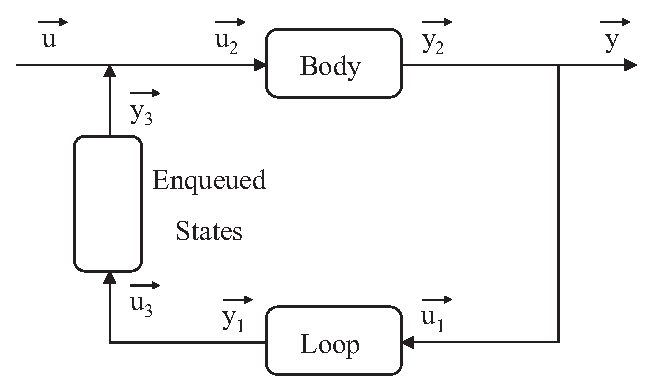
\includegraphics[width=3.0in]{figures/feedback2.eps}
  \caption{Labelled feedback loop}
  \label{fig:feedback2}
\end{figure}

    From figure \ref{fig:feedback2} it is apparent that $\vec{\mathbf{u_3}} =
\vec{\mathbf{y_1}}$, $\vec{\mathbf{y}} = \vec{\mathbf{y_2}} =
\vec{\mathbf{u_1}}$, and $\vec{\mathbf{u_2}}$ is composed of
$\vec{\mathbf{u}}$ and $\vec{\mathbf{u_3}}$. We can write the
equations for the body block as:
\begin{eqnarray*}
\vec{\dot{\mathbf{x_2}}} & = & \mathbf{A_2} \vec{\mathbf{x_2}} +
\mathbf{B_2} \vec{\mathbf{u_2}} = \mathbf{A_2}\vec{\mathbf{x_2}} +
\mathbf{B_{2\_1}} \vec{\mathbf{u}} + \mathbf{B_{2\_2}}
\vec{\mathbf{y_3}} = \mathbf{A_2}\vec{\mathbf{x_2}} +
\mathbf{B_{2\_1}} \vec{\mathbf{u}} + \mathbf{B_{2\_2}}
\mathbf{C_3} \vec{\mathbf{x_3}} \\
\vec{\mathbf{y_2}} & = & \mathbf{C_2} \vec{\mathbf{x_2}} +
\mathbf{D_2} \vec{\mathbf{u_2}} = \mathbf{C_2}\vec{\mathbf{x_2}} +
\mathbf{D_{2\_1}} \vec{\mathbf{u}} + \mathbf{D_{2\_2}}
\vec{\mathbf{y_3}} = \mathbf{C_2}\vec{\mathbf{x_2}} +
\mathbf{D_{2\_1}} \vec{\mathbf{u}} + \mathbf{D_{2\_2}}
\mathbf{C_3} \vec{\mathbf{x_3}}
\end{eqnarray*}

    Since $\vec{\mathbf{y}} = \vec{\mathbf{y_2}}$, we have written
the output of the feedback loop and the update for
$\vec{\mathbf{x_2}}$ in terms of the input to the feedback loop
and the state vectors. For the updates to $\vec{\mathbf{x_1}}$ and
$\vec{\mathbf{x_3}}$ we can write:
\begin{eqnarray*}
\vec{\dot{\mathbf{x_1}}} & = & \mathbf{A_1} \vec{\mathbf{x_1}} +
\mathbf{B_1} \vec{\mathbf{u_1}} = \mathbf{A_1}\vec{\mathbf{x_1}} +
\mathbf{B_1} \vec{\mathbf{y}} =  \mathbf{A_1}\vec{\mathbf{x_1}} +
\mathbf{B_1}(\mathbf{C_2}\vec{\mathbf{x_2}} + \mathbf{D_{2\_1}}
\vec{\mathbf{u}} + \mathbf{D_{2\_2}} \mathbf{C_3}
\vec{\mathbf{x_3}}) \\
& = & \mathbf{A_1}\vec{\mathbf{x_1}} +
\mathbf{B_1}\mathbf{C_2}\vec{\mathbf{x_2}} + \mathbf{B_1}
\mathbf{D_{2\_1}} \vec{\mathbf{u}} + \mathbf{B_1}
\mathbf{D_{2\_2}} \mathbf{C_3} \vec{\mathbf{x_3}} \\ \\
\vec{\dot{\mathbf{x_3}}} & = & \mathbf{A_3} \vec{\mathbf{x_3}} +
\mathbf{B_3} \vec{\mathbf{u_3}} = \mathbf{A_3}\vec{\mathbf{x_3}} +
\mathbf{B_3} \vec{\mathbf{y_1}} =  \mathbf{A_3}\vec{\mathbf{x_3}}
+ \mathbf{B_3}(\mathbf{C_1}\vec{\mathbf{x_1}} + \mathbf{D_1}
\vec{\mathbf{u_1}}) \\
& = & \mathbf{A_3}\vec{\mathbf{x_3}} +
\mathbf{B_3}(\mathbf{C_1}\vec{\mathbf{x_1}} +
\mathbf{D_1}\vec{\mathbf{y}}) = \mathbf{A_3}\vec{\mathbf{x_3}} +
\mathbf{B_3}(\mathbf{C_1}\vec{\mathbf{x_1}} +
\mathbf{D_1}(\mathbf{C_2}\vec{\mathbf{x_2}} + \mathbf{D_{2\_1}}
\vec{\mathbf{u}} + \mathbf{D_{2\_2}} \mathbf{C_3}
\vec{\mathbf{x_3}})) \\
& = & \mathbf{A_3}\vec{\mathbf{x_3}} +
\mathbf{B_3}\mathbf{C_1}\vec{\mathbf{x_1}} +
\mathbf{B_3}\mathbf{D_1}\mathbf{C_2}\vec{\mathbf{x_2}} +
\mathbf{B_3}\mathbf{D_1}\mathbf{D_{2\_1}} \vec{\mathbf{u}} +
\mathbf{B_3}\mathbf{D_1}\mathbf{D_{2\_2}} \mathbf{C_3}
\vec{\mathbf{x_3}}
\end{eqnarray*}

    For the input and output rates we have $o = E * w_2$
and $u = u_2$. We use the states of all three representations, so
$s = s_1 + s_2 + s_3$ and $\overrightarrow{\mathbf{initVec}} =
\left [ \begin{array} {c} \overrightarrow{\mathbf{initVec_1}} \\
\overrightarrow{\mathbf{initVec_2}} \\
\overrightarrow{\mathbf{initVec_3}} \end{array} \right ]$. For
simplicity, we do not consider a loop or body block with
initialization matrices.

\subsection{Representation Changes}

\subsubsection{Expansion}

    We may want to run a block multiple times in order to
properly combine it with other blocks. For example, suppose block
$B_1$ inputs three items and outputs two items, and block $B_2$
inputs five items and outputs seven items. In order to combine
these blocks in a pipeline, $B_1$ must run five times (in order to
output ten items) and $B_2$ must run two times (in order to input
ten items). Therefore, we need to have a method to expand a
representation so that it models a block running multiple times,
rather than once.

    Consider the state-space equation pair, where $\vec{\mathbf{u_1}}$ and
$\vec{\mathbf{y_1}}$ are the first set of inputs and outputs, and
$\vec{\mathbf{x}}$ is the original state vector:
\begin{eqnarray*}
\vec{\dot{\mathbf{x}}} & = & \mathbf{A}\vec{\mathbf{x}} + \mathbf{B}\vec{\mathbf{u_1}} \\
\vec{\mathbf{y_1}} & = & \mathbf{C}\vec{\mathbf{x}} +
\mathbf{D}\vec{\mathbf{u_1}}
\end{eqnarray*}

    If we run the block again, the equation pair in terms of the
original state vector $\vec{\mathbf{x}}$ and the next set of
inputs and outputs ($\vec{\mathbf{u_2}}$ and $\vec{\mathbf{y_2}}$)
is:
\begin{eqnarray*}
\vec{\dot{\mathbf{x}}} & = & \mathbf{A}(\mathbf{A}\vec{\mathbf{x}}
+
\mathbf{B}\vec{\mathbf{u_1}}) + \mathbf{B}\vec{\mathbf{u_2}} \\
\vec{\mathbf{y_2}} & = & \mathbf{C}(\mathbf{A}\vec{\mathbf{x}} +
\mathbf{B}\vec{\mathbf{u_1}}) + \mathbf{D}\vec{\mathbf{u_2}}
\end{eqnarray*}

Simplifying yields:
\begin{eqnarray*}
\vec{\dot{\mathbf{x}}} & = & \mathbf{A}^2\vec{\mathbf{x}} +
\mathbf{AB}\vec{\mathbf{u_1}} + \mathbf{B}\vec{\mathbf{u_2}} \\
\vec{\mathbf{y_2}} & = & \mathbf{CA}\vec{\mathbf{x}} +
\mathbf{CB}\vec{\mathbf{u_1}} + \mathbf{D}\vec{\mathbf{u_2}}
\end{eqnarray*}

    Let $\vec{\mathbf{u}}$ be the combined input vector
($\vec{\mathbf{u}} = \left [ \begin{array} {c} \vec{\mathbf{u_1}}
\\ \vec{\mathbf{u_2}} \end{array} \right ]$) and $\vec{\mathbf{y}}$ be the combined output vector
($\vec{\mathbf{y}} = \left [ \begin{array} {c} \vec{\mathbf{y_1}}
\\ \vec{\mathbf{y_2}} \end{array} \right ]$). The representation in terms of these two
vectors is:
\begin{eqnarray*}
\vec{\dot{\mathbf{x}}} & = & \mathbf{A_2}\vec{\mathbf{x}} + \mathbf{B_2}\vec{\mathbf{u}} \\
\vec{\mathbf{y}} & = & \mathbf{C_2}\vec{\mathbf{x}} + \mathbf{D_2}\vec{\mathbf{u}} \\
\mathbf{A_2} & = & \mathbf{A}^2 \\
\mathbf{B_2} & = & \left [ \begin{array} {cc} \mathbf{AB} & \mathbf{B} \end{array} \right ] \\
\mathbf{C_2} & = & \left [ \begin{array} {c} \mathbf{C} \\
\mathbf{CA} \end{array} \right ] \\
\mathbf{D_2} & = & \left [ \begin{array} {cc} \mathbf{D} & \mathbf{0} \\
\mathbf{CB} & \mathbf{D} \end{array} \right ]
\end{eqnarray*}

    This new representation corresponds to a block that upon
every execution runs the old block twice. By induction, a general
formula for running a block n times is:
\begin{eqnarray}
\mathbf{A_n} & = & \mathbf{A}^n \\
\mathbf{B_n} & = & \left [ \begin{array} {ccccc} \mathbf{A}^{n-1}
\mathbf{B} & \mathbf{A}^{n-2} \mathbf{B} & ...  & \mathbf{AB} &
\mathbf{B} \end{array} \right ] \\
\mathbf{C_n} & = & \left [ \begin{array} {c} \mathbf{C} \\
\mathbf{CA} \\
... \\
\mathbf{CA^{n-2}} \\
\mathbf{CA^{n-1}} \end{array} \right ] \\
\mathbf{D_n} & = & \left [ \begin{array} {ccccccc}
\mathbf{D} & \mathbf{0} & \mathbf{0} & ... & \mathbf{0} & \mathbf{0} & \mathbf{0} \\
\mathbf{CB} & \mathbf{D} & \mathbf{0} & ... & \mathbf{0} & \mathbf{0} & \mathbf{0} \\
\mathbf{CAB} & \mathbf{CB} & \mathbf{D} & ... & \mathbf{0} & \mathbf{0} & \mathbf{0} \\
... & ... & ... & ... & ... & ... & ... \\
\mathbf{CA}^{n-4} \mathbf{B} & \mathbf{CA}^{n-5} \mathbf{B} &
\mathbf{CA}^{n-6} \mathbf{B} & ... & \mathbf{D} & \mathbf{0} & \mathbf{0} \\
\mathbf{CA}^{n-3} \mathbf{B} & \mathbf{CA}^{n-4} \mathbf{B} &
\mathbf{CA}^{n-5} \mathbf{B} & ... & \mathbf{CB} & \mathbf{D} & \mathbf{0} \\
\mathbf{CA}^{n-2} \mathbf{B} & \mathbf{CA}^{n-3} \mathbf{B} &
\mathbf{CA}^{n-4} \mathbf{B} & ... & \mathbf{CAB} & \mathbf{CB} &
\mathbf{D} \end{array} \right ]
\end{eqnarray}

    Since initializations are not affected, $\overrightarrow{\mathbf{initVec}}$,
$\mathbf{preA}$, $\mathbf{preB}$, $stored$, and $o_{pre}$ remain
unchanged from the initial representation. Since the number of
states is not changed, $s$ remains the same. The new
representation runs the old representation $n$ times, so $u_{new}
= n * u_{old}$, $o_{new} = n * o_{old}$.

    As mentioned in the pipeline combination section, we may need
to run a block $n$ times, in addition to its initialization
matrices, for the purpose of initializing the full pipeline. We
denoted the matrices for doing this as $\mathbf{A^e}$,
$\mathbf{B^e}$, $\mathbf{C^e}$, and $\mathbf{D^e}$. If the block
being run $n$ times does not need initialization, the calculation
for these four matrices is exactly the same as described in
equations (3.2)-(3.5). Otherwise, we must make some slight
modifications:
\begin{eqnarray}
\mathbf{A^e} & = & \mathbf{A}^n \mathbf{A_{pre}} \\
\mathbf{B^e} & = & \left [ \begin{array} {ccccc} \mathbf{A^n}
\mathbf{B_{pre}} & \mathbf{A^{n-1}} \mathbf{B} & \mathbf{A^{n-2}}
\mathbf{B} & ... & \mathbf{B}
\end{array} \right ] \\
\mathbf{C^e} & = & \left [ \begin{array} {c} \mathbf{C} \mathbf{A_{pre}} \\
\mathbf{C} \mathbf{A} \mathbf{A_{pre}} \\ ... \\
\mathbf{C} \mathbf{A^{n-1}} \mathbf{A_{pre}} \end{array} \right ] \\
\mathbf{D^e} & = & \left [ \begin{array} {cccccccc} \mathbf{C}
\mathbf{B_{pre}} & \mathbf{D} & \mathbf{0} &
\mathbf{0} & ... & \mathbf{0} & \mathbf{0} \\
\mathbf{C} \mathbf{A} \mathbf{B_{pre}} & \mathbf{CB} &
\mathbf{D} & \mathbf{0} & ... & \mathbf{0} & \mathbf{0} \\
\mathbf{C} \mathbf{A}^2 \mathbf{B_{pre}} & \mathbf{CAB} &
\mathbf{CB} & \mathbf{D} & ... & \mathbf{0} & \mathbf{0} \\
... & ... & ... & ... & ... & ... \\
\mathbf{C} \mathbf{A^{n-1}} \mathbf{B_{pre}} & \mathbf{CA}^{n-2}
\mathbf{B} & \mathbf{CA}^{n-3} \mathbf{B} &
\mathbf{CA}^{n-3} \mathbf{B} & ... & \mathbf{CB} & \mathbf{D} \\
 \end{array} \right ]
\end{eqnarray}

\subsubsection{Increasing the number of Stored Inputs}

    As mentioned in Section 3.3.1, it may be necessary to changed the
stored inputs in a representation in order to combine it with
another representation in a pipeline. Suppose we want to change
the number of stored inputs from $oldStored$ to $newStored$.
Consider what happens in the old representation, with $oldStored$
stored input variables. The filter accesses $peek(0)$, $peek(1)$,
... $peek(oldStored-1)$ from the $oldStored$ stored input state
variables. The $o$ inputs to the filter are $peek(oldStored)$,
$peek(oldStored+1)$, ... $peek(oldStored+o-1)$. Now we want to add
$newStored-oldStored$ stored input variables, so that the total
$newStored$ stored input variables represent $peek(0)$, $peek(1)$,
... $peek(newStored-1)$, and the $o$ inputs to the filter are
$peek(newStored)$, $peek(newStored+1)$, ... $peek(newStored+o-1)$.
Therefore, any references in the original representation to
$peek(0)$, $peek(1)$, ... $peek(oldStored-1)$ remain the same,
while references to $peek(oldStored)$, $peek(oldStored)$, ...
$peek(oldStored+o-1)$ must be changed.

    The old representation was:
\begin{eqnarray*}
\left [ \begin{array} {c} \vec{\dot{\mathbf{x_1}}} \\
\vec{\dot{\mathbf{x_2}}}
\end{array} \right ] & = & \left [ \begin{array} {cc} \mathbf{A_{11}} & \mathbf{A_{12}} \\
\mathbf{A_{21}} & \mathbf{A_{22}} \end{array} \right ] \left [
\begin{array} {c} \vec{\mathbf{x_1}} \\ \vec{\mathbf{x_2}} \end{array} \right ]
 + \left [ \begin{array} {cc} \mathbf{B_{11}} & \mathbf{B_{12}} \\
\mathbf{B_{21}} & \mathbf{B_{22}} \end{array} \right ] \left[
\begin{array} {c} \vec{\mathbf{u_1}} \\ \vec{\mathbf{u_2}} \end{array} \right ] \\
\vec{\mathbf{y}} & = & \left [ \begin{array} {cc} \mathbf{C_1} &
\mathbf{C_2} \end{array} \right ] \left [
\begin{array} {c} \vec{\mathbf{x_1}} \\ \vec{\mathbf{x_2}} \end{array} \right ] +
\left [ \begin{array} {cc} \mathbf{D_1} & \mathbf{D_2}
\end{array} \right ] \left [ \begin{array} {c} \vec{\mathbf{u_1}} \\
\vec{\mathbf{u_2}} \end{array} \right ]
\end{eqnarray*}

    We have divided the state vector $\vec{\mathbf{x}}$ into the non-stored input variables ($\vec{\mathbf{x_1}}$)
and the stored input variables ($\vec{\mathbf{x_2}}$), and divided
the input vector $\vec{\mathbf{u}}$ into the first
$newStored-oldStored$ inputs ($\vec{\mathbf{u_1}}$) and the
remaining inputs ($\vec{\mathbf{u_2}}$). We will assume
$newStored-oldStored <= o$ (If not we can run this algorithm
multiple times). The matrices $\mathbf{A}$, $\mathbf{B}$,
$\mathbf{C}$, and $\mathbf{D}$ are put into block-matrix form
according to the state and input vector divisions.

    In our new representation, we use $\vec{\mathbf{x_3}}$ to denote the
added $newStored - oldStored$ states. As mentioned early,
references to the first $oldStored$ stored input states
($\vec{\mathbf{x_2}}$) remain the same. Additionally, references
to the non-input states ($\vec{\mathbf{x_1}}$) also remain the
same. Our new representation so far is:
\begin{eqnarray*}
\left [ \begin{array} {c} \vec{\dot{\mathbf{x_1}}} \\ \vec{\dot{\mathbf{x_2}}} \\
\vec{\dot{\mathbf{x_3}}}
\end{array} \right ] & = & \left [ \begin{array} {ccc} \mathbf{A_{11}} & \mathbf{A_{12}} & ? \\
\mathbf{A_{21}} & \mathbf{A_{22}} & ? \\ ? & ? & ?
\end{array} \right ] \left [
\begin{array} {c} \vec{\mathbf{x_1}} \\ \vec{\mathbf{x_2}} \\ \vec{\mathbf{x_3}} \end{array} \right ]
 + \left [ \begin{array} {cc} ? & ? \\ ? & ? \\ ? & ? \end{array} \right ] \left[
\begin{array} {c} \vec{\mathbf{u_1}} \\ \vec{\mathbf{u_2}} \end{array} \right ] \\
\vec{\mathbf{y}} & = & \left [ \begin{array} {ccc} \mathbf{C_1} &
\mathbf{C_2} & ? \end{array} \right ] \left [
\begin{array} {c} \vec{\mathbf{x_1}} \\ \vec{\mathbf{x_2}} \\ \vec{\mathbf{x_3}} \end{array} \right ] +
\left [ \begin{array} {cc} ? & ?
\end{array} \right ] \left [ \begin{array} {c} \vec{\mathbf{u_1}} \\
\vec{\mathbf{u_2}} \end{array} \right ]
\end{eqnarray*}

    The ? indicates yet to be determined entries. In the old
representation, the first $newStored-oldStored$ input elements
($u_1$) were $peek(oldStored)$ ... $peek(newStored-1)$. In the new
representation, these values are stored as states ($x_3$).
Therefore, any matrix block that was previously multiplied by
$u_1$ should be multiplied by $x_2$ instead. Now the new
representation is:
\begin{eqnarray*}
\left [ \begin{array} {c} \vec{\dot{\mathbf{x_1}}} \\ \vec{\dot{\mathbf{x_2}}} \\
\vec{\dot{\mathbf{x_3}}}
\end{array} \right ] & = & \left [ \begin{array} {ccc} \mathbf{A_{11}} &
\mathbf{A_{12}} & \mathbf{B_{11}} \\ \mathbf{A_{21}} &
\mathbf{A_{22}} & \mathbf{B_{21}} \\ ? & ? & ?  \end{array} \right
] \left [
\begin{array} {c} \vec{\mathbf{x_1}} \\ \vec{\mathbf{x_2}} \\ \vec{\mathbf{x_3}} \end{array} \right ]
 + \left [ \begin{array} {cc} ? & ? \\ ? & ? \\ ? & ? \end{array} \right ] \left[
\begin{array} {c} \vec{\mathbf{u_1}} \\ \vec{\mathbf{u_2}} \end{array} \right ] \\
\vec{\mathbf{y}} & = & \left [ \begin{array} {ccc} \mathbf{C_1} &
\mathbf{C_2} & \mathbf{D_1}  \end{array} \right ] \left [
\begin{array} {c} \vec{\mathbf{x_1}} \\ \vec{\mathbf{x_2}} \\ \vec{\mathbf{x_3}} \end{array} \right ] +
\left [ \begin{array} {cc} ? & ?
\end{array} \right ] \left [ \begin{array} {c} \vec{\mathbf{u_1}} \\
\vec{\mathbf{u_2}} \end{array} \right ]
\end{eqnarray*}

    In the old representation, the remaining $o-(newStored-oldStored)$ input elements
($u_2$) were $peek(newStored)$ ... $peek(o+oldStored-1)$. In the
new representation, these are the first $o-(newStored-oldStored)$
input elements. We divide the input vector into the first
$o-(newStored-oldStored)$ elements ($\vec{u_{1'}}$) and the
remaining $newStored-oldStored$ elements ($\vec{u_{2'}}$). Any
matrix block that was previously multiplied by
$\vec{\mathbf{u_2}}$ should be multiplied by $\vec{u_{1'}}$
instead. Additionally, there is no dependence on $\vec{u_{2'}}$ by
$\vec{\mathbf{x_1}}$, $\vec{\mathbf{x_2}}$, or $\vec{\mathbf{y}}$.
The new representation is:
\begin{eqnarray*}
\left [ \begin{array} {c} \vec{\dot{\mathbf{x_1}}} \\ \vec{\dot{\mathbf{x_2}}} \\
\vec{\dot{\mathbf{x_3}}} \end{array} \right ] & = & \left [
\begin{array} {ccc} \mathbf{A_{11}} & \mathbf{A_{12}} &
\mathbf{B_{11}} \\ \mathbf{A_{21}} & \mathbf{A_{22}} &
\mathbf{B_{21}} \\ ? & ? & ? \end{array} \right ] \left [
\begin{array} {c} \vec{\mathbf{x_1}} \\ \vec{\mathbf{x_2}} \\ \vec{\mathbf{x_3}} \end{array} \right ]
+ \left [ \begin{array} {cc} \mathbf{B_{12}} & \mathbf{0} \\
\mathbf{B_{22}} & \mathbf{0} \\ ? & ? \end{array} \right ] \left[
\begin{array} {c} \vec{u_{1'}} \\ \vec{u_{2'}} \end{array} \right ] \\
\vec{\mathbf{y}} & = & \left [ \begin{array} {ccc} \mathbf{C_1} &
\mathbf{C_2} & \mathbf{D_1} \end{array} \right ] \left [
\begin{array} {c} \vec{\mathbf{x_1}} \\ \vec{\mathbf{x_2}} \\ \vec{\mathbf{x_3}} \end{array} \right ] +
\left [ \begin{array} {cc} \mathbf{D_2} & \mathbf{0}
\end{array} \right ] \left [ \begin{array} {c} \vec{u_{1'}} \\
\vec{u_{2'}} \end{array} \right ]
\end{eqnarray*}

    The entries for the state update $\vec{\dot{\mathbf{x_3}}}$ remain to be
determined. Any stored input variable representing $peek(i)$ must
get updated by $peek(i+o)$. $\vec{\dot{\mathbf{x_3}}}$ is
$peek(oldStored)$ ... $peek(newStored-1)$, so it must be updated
by $peek(o+oldStored)$ ... $peek(o+newStored-1)$. This is
precisely $\vec{u_{2'}}$, so the final new representation is:
\begin{eqnarray*}
\left [ \begin{array} {c} \vec{\dot{\mathbf{x_1}}} \\ \vec{\dot{\mathbf{x_2}}} \\
\vec{\dot{\mathbf{x_3}}}
\end{array} \right ] & = & \left [ \begin{array} {ccc} \mathbf{A_{11}} &
\mathbf{A_{12}} & \mathbf{B_{11}} \\ \mathbf{A_{21}} &
\mathbf{A_{22}} & \mathbf{B_{21}} \\ \mathbf{0} & \mathbf{0} & \mathbf{0} \\
\end{array} \right ] \left [ \begin{array} {c} \vec{\mathbf{x_1}} \\ \vec{\mathbf{x_2}} \\
\vec{\mathbf{x_3}} \end{array} \right ] + \left [ \begin{array}
{cc} \mathbf{B_{12}} & \mathbf{0} \\ \mathbf{B_{22}} & \mathbf{0} \\ \mathbf{0} & \mathbf{I} \\
\end{array} \right ] \left[ \begin{array} {c} \vec{u_{1'}} \\ \vec{u_{2'}} \end{array} \right ] \\
\vec{\mathbf{y}} & = & \left [ \begin{array} {ccc} \mathbf{C_1} &
\mathbf{C_2} & \mathbf{D_1} \end{array} \right ] \left [
\begin{array} {c} \vec{\mathbf{x_1}} \\ \vec{\mathbf{x_2}} \\ \vec{\mathbf{x_3}} \end{array} \right ] +
\left [ \begin{array} {cc} \mathbf{D_2} & \mathbf{0}
\end{array} \right ] \left [ \begin{array} {c} \vec{u_{1'}} \\
\vec{u_{2'}} \end{array} \right ]
\end{eqnarray*}

    Similarly, let the original initialization equation be:
\begin{eqnarray*}
\left [ \begin{array} {c} \vec{\dot{\mathbf{x_1}}} \\
\vec{\dot{\mathbf{x_2}}} \end{array} \right ] = \left [
\begin{array} {cc} \mathbf{A_{pre11}} & \mathbf{A_{pre12}} \\
\mathbf{0} & \mathbf{0} \end{array} \right ] \left [
\begin{array} {c} \vec{\mathbf{x_1}} \\ \vec{\mathbf{x_2}}
\end{array} \right ] + \left [ \begin{array} {cc} \mathbf{B_{pre11}} & \mathbf{B_{pre12}} \\
\mathbf{I} & \mathbf{0} \end{array} \right ] \left [ \begin{array}
{c} \vec{\mathbf{u_{pre1}}} \\ \vec{\mathbf{u_{pre2}}}
\end{array} \right ]
\end{eqnarray*}

    Where $\vec{\mathbf{u_{pre1}}}$ has length $oldStored$, and
$\vec{\mathbf{u_{pre2}}}$ has length $o_{pre} - oldStored$. Now we
simply consider $\vec{\mathbf{u_{pre1}}}$ to have length
$newStored$ and $\vec{\mathbf{u_{pre2}}}$ to have length $o_{pre}
- newStored$. If $o_{pre} < newStored$, we set $o_{pre} =
newStored$. Then the initialization equation is the same as
before, except the original stored input states
($\vec{\mathbf{x_2}})$ are replaced by the new stored input states
($\left [ \begin{array} {c} \vec{\mathbf{x_2}} \\
\vec{\mathbf{x_3}} \end{array} \right ]$).

    We have derived $\mathbf{A}$, $\mathbf{B}$, $\mathbf{C}$, $\mathbf{D}$,
$\mathbf{A_{pre}}$, and $\mathbf{B_{pre}}$ for the new
representation. Clearly, $stored = newStored$ and $o_{pre} =
o_{preold} + newStored-oldStored$. The input/output rate remains
the same, so $o = o_{old}$ and $u = u_{old}$. We have added
$newStored-oldStored$ total states, so $s = s_{old} + (newStored -
oldStored)$ and $\overrightarrow{\mathbf{initVec}} =
\left [ \begin{array} {c} \overrightarrow{\mathbf{initVec_1}} \\
\overrightarrow{\mathbf{initVec_2}} \\ \overrightarrow{\mathbf{0}}
\end{array} \right ]$.

\subsection{Replacement}

    Once we have combined filters to a single representation and
performed optimizations on it (see Section 4), we would like to
convert it to StreamIt code. Given a representation $\mathrm{R}$
we can create the following StreamIt filter:

\begin{scriptsize}
\begin{singlespace}
\begin{verbatim}
float -> float filter replacementFilter() {
  float x0, ... , x{s-1};

  prework push 0 pop preu peek preu {
    x0 = preA[0,0]*x0 + ... + preA[0,s-1]*x{s-1} + preB[0,0]*peek(0) + ... + preB[0,preu-1]*peek(preu-1);
    x1 = preA[1,0]*x0 + ... + preA[1,s-1]*x{s-1} + preB[1,0]*peek(0) + ... + preB[1,preu-1]*peek(preu-1);
    ...
    x{s-1} = preA[s-1,0]*x0 + ... + preA[s-1,s-1]*x{s-1} + preB[s-1,0]*peek(0) + ... + preB[s-1,preu-1]*peek(preu-1);
  }

  work push u pop o peek o {
    float x0_temp, ... , x{s-1}_temp;

    push(C[0,0]*x0 + ... + C[0,s-1]*x{s-1} + D[0,0]*peek(0) + ... + D[0,o-1]*peek(o-1));
    push(C[1,0]*x0 + ... + C[1,s-1]*x{s-1} + D[1,0]*peek(0) + ... + D[1,o-1]*peek(o-1));
    ...
    push(C[u,0]*x0 + ... + C[u,s-1]*x{s-1} + D[u,0]*peek(0) + ... + D[u,o-1]*peek(o-1));

    x0_temp = A[0,0]*x0 + ... + A[0,s-1]*x{s-1} + B[0,0]*peek(0) + ... + B[0,o-1]*peek(o-1);
    x1_temp = A[1,0]*x0 + ... + A[1,s-1]*x{s-1} + B[1,0]*peek(0) + ... + B[1,o-1]*peek(o-1);
    ...
    x{s-1}_temp = A[s-1,0]*x0 + ... + A[s-1,s-1]*x{s-1} + B[s-1,0]*peek(0) + ... + B[s-1,o-1]*peek(o-1);

    x0 = x0_temp;
    ...
    x{s-1} = x{s-1}_temp;

    pop(); pop(); ... pop(); // o pops
  }
}
\end{verbatim}
\end{singlespace}
\end{scriptsize}

    We make two modifications to this filter. If a matrix entry is
zero, any term involving that matrix entry is not placed in the
filter. If a matrix entry is one, the multiplication of a peek or
variable by this matrix entry is removed.

  \mysection{Optimization}
\label{sec:optimization}

There are two types of optimizations we consider.  The first is to
remove extraneous state variables from the linear state space
representation. This reduces the memory allocation for a program and
reduces the number of loads and stores executed, which are typically
slow and power-hungry operations. It also eliminates computations that
involve the removed states.  The second optimization is to reduce the
parametrization of a state space representation, by changing the
representation to one with more zero and one entries in its
matrices. This directly eliminates computations, since all
multiplications by zero or one are not processed by the replacement
algorithm.

\mysubsection{State-Space Transformations}

    For any state space equation pair, there are an infinite
number of transformations to an equivalent state space system.
These transformations involve a change of basis of the state
vector $\vec{\mathbf{x}}$ to $\mathbf{T} \vec{\mathbf{x}}$, where
$\mathbf{T}$ is an invertible matrix. Consider the state-update
equation $\vec{\dot{\mathbf{x}}} = \mathbf{A} \vec{\mathbf{x}} +
\mathbf{B} \vec{\mathbf{u}}$. Multiplying the entire equation by
$\mathbf{T}$ yields:
\starteqnstar
\mathbf{T} \vec{\dot{\mathbf{x}}} = \mathbf{TA} \vec{\mathbf{x}} +
\mathbf{TB} \vec{\mathbf{u}}
\doneeqnstar

\vspace{-9pt} Since $\mathbf{T}^{-1} \mathbf{T} = \mathbf{I}$, we can write:
\starteqnstar
\mathbf{T} \vec{\dot{\mathbf{x}}} & = & \mathbf{TA}
(\mathbf{T}^{-1} \mathbf{T}) \vec{\mathbf{x}} + \mathbf{TB}
\vec{\mathbf{u}} = \mathbf{TA}
\mathbf{T}^{-1} (\mathbf{T} \vec{\mathbf{x}}) + \mathbf{TB} \vec{\mathbf{u}} \\
\vec{\mathbf{y}} & = & \mathbf{C} (\mathbf{T}^{-1} \mathbf{T})
\vec{\mathbf{x}} + \mathbf{D} \vec{\mathbf{u}} = \mathbf{C}
\mathbf{T}^{-1} (\mathbf{T} \vec{\mathbf{x}}) + \mathbf{D}
\vec{\mathbf{u}}
\doneeqnstar

\vspace{-9pt} Where we have introduced the output equation as well. Let
$\vec{\mathbf{z}} = \mathbf{T} \vec{\mathbf{x}}$.
$\vec{\mathbf{z}}$ is a new state vector related to the old state
vector $\vec{\mathbf{x}}$ by the change of basis $\mathbf{T}$.
Substituting into the equations above we get:
\starteqnstar
\vec{\dot{\mathbf{z}}} & = & \mathbf{TA} \mathbf{T}^{-1} \vec{\mathbf{z}} + \mathbf{TB} \vec{\mathbf{u}} \\
\vec{\mathbf{y}} & = & \mathbf{C} \mathbf{T}^{-1}\vec{\mathbf{z}}
+ \mathbf{D}\vec{\mathbf{u}}
\doneeqnstar

\vspace{-9pt} This is precisely the original state space equation pair,
with $\mathbf{A}$, $\mathbf{B}$, and $\mathbf{C}$ transformed to
$\mathbf{T} \mathbf{A} \mathbf{T}^{-1}$, $\mathbf{T} \mathbf{B}$,
and $\mathbf{C} \mathbf{T}^{-1}$, respectively.

    For a StreamIt state space representation $\mathrm{R}$, we must
determine how the other values change. The initialization state
update equation is essentially the same as the regular state
update equation, so $\mathbf{A_{pre}}$ and $\mathbf{B_{pre}}$ are
transformed to $\mathbf{T} \mathbf{A_{pre}} \mathbf{T}^{-1}$ and
$\mathbf{T} \mathbf{B}$ respectively. Since the old state vector
$\vec{\mathbf{x}}$ is multiplied by $\mathbf{T}$, the old initial
state vector is multiplied by $\mathbf{T}$. The number of states,
inputs, and outputs is the same, so $s$, $o$, and $u$ are
unchanged.

\mysubsection{State Removal}
\label{sec:state-removal}

    There are two types of states that can be removed from a
state space system without changing its behavior: unreachable and
unobservable states. Informally, unreachable states are unaffected by
inputs and unobservable states have no effect on outputs. More
formally, the set of states in a system can be divided into reachable
and unreachable states where:
\begin{enumerate}
\vspace{\itemshrink} \item The unreachable states are not updated by any of the
reachable states.

\vspace{\itemshrink} \item The unreachable states are not updated by any inputs.
\vspace{\itemshrink} \end{enumerate}

    In terms of the state space equation pair, this means $\mathbf{A}[i,j] =
0, \mathbf{B}[i,k] = 0$ where $i$ is the row of an unreachable
state, $j$ is the column of a reachable state, and $k$ is any of
the inputs.
    If all the unreachable states are initially zero, they
remain zero because they are not updated by a non-zero value
(either a reachable state or an input). Therefore, all unreachable
states that are not initialized can be removed from a
representation, since they do not effect the reachable states or
the outputs.

    The set of states in a system can also be divided into
observable and unobservable states where:
\begin{enumerate}
\vspace{\itemshrink} \item The observable states are not updated by any of the
unobservable states.

\vspace{\itemshrink} \item The outputs do not depend on the unobservable states.
\vspace{\itemshrink} \end{enumerate}

    In terms of the state space equation pair, this means $\mathbf{C}[i,j] =
0, \mathbf{D}[k,j] = 0$ where $j$ is the column of an observable
state, $i$ is the row of an unobservable state, and $k$ is any of
the outputs.
    The unobservable states are not used to update the observable
states and are not used to determine the outputs. Therefore, all
unobservable states can be removed from a representation
(regardless of their initial values).

    A simple algorithm to isolate the unreachable and unobservable
states in a system by use of transformations is explained in
\cite{Mayne}. The algorithm works as follows: perform row
operations on the augmented matrix $\left [ \begin{array} {cc}
\mathbf{A} & \mathbf{B} \end{array} \right ]$ to put it into a
type of row-echelon form\footnote{A matrix is in standard row-echelon
form if the first non-zero entry in each row is a 1 (called the
leading 1) and the leading 1 in a higher row is to the left of the
leading 1 in a lower row. For our type of row-echelon form, the
\emph{last} non-zero entry in each row is a 1 (call it the ending 1)
and the ending 1 in a higher row is to the left of the ending 1 in a
lower row.}, and perform the corresponding inverse column operations
on $\mathbf{A}$ and $\mathbf{C}$ to keep the system equivalent to the
original. (Performing a row operation on a matrix is equivalent to
left multiplying it by some invertible matrix, and performing a column
operation on a matrix is equivalent to right multiplying it by some
invertible matrix).  Once the augmented matrix is in the desired form,
row $i$ of the combined matrix represents an unreachable state if
there are no non-zero entries past the $i^{th}$ column. For
unobservable states, the combined matrix $\left [ \begin{array} {cc}
\mathbf{A}^T & \mathbf{C}^T
\end{array} \right ]$ is operated on instead.

    Using this algorithm, we can find the entire set of unobservable
states and remove them all. The only exceptions are those
unobservable states that affect observable states in the
initialization matrix $\matrix{A_{pre}}$. If $j$ is the column of
an observable state then we must have $\mathbf{A_{pre}}[i,j] = 0$
for all values of $i$, where $i$ is the row of an observable
state. Otherwise, the unobservable state $j$ cannot be removed,
because it affects at least one observable state, and therefore
may affect the outputs.

    More care must be taken when removing unreachable states. If an
unreachable state has a non-zero starting value, or is affected by
the initialization matrices, it cannot be removed. In either of
these cases, the unreachable state may attain a non-zero value,
and therefore may have an affect on the reachable states and/or
outputs. Additionally, an unreachable state $x_1$ that is updated
by a different unreachable state $x_2$ that cannot be removed may
eventually have a non-zero value, even if it ($x_1$) is initially
zero. Therefore, the unreachable state $x_1$ cannot be removed as
well.

    The last case may cause problems when trying to remove
unreachable states. If an unreachable state $x_1$ is updated by
unreachable states $x_2$ and $x_3$, we must check if those states
can be removed before determining if state $x_1$ can be removed.
If one of those states, say $x_2$, depends on $x_1$, we must
determine if $x_1$ can be removed before determining whether $x_2$
can be removed - resulting in an impossible `loop-like'
determination. Clearly, a more robust approach is necessary.

    Suppose we have found the set of unreachable states and they
form the first $k$ states of the state vector (we can do both of
these steps by isolating the unreachable states, then moving them
to the top of the state vector if necessary). Consider the
sub-matrix $\mathbf{A}[1:k;1:k]$ consisting of the first k rows
and first k columns of $\mathbf{A}$. This sub-matrix represents
how the unreachable states are updated based on each other.
Suppose this sub-matrix is in upper-triangular form, which means
that all entries below the main diagonal are zero. We can remove
states in the following manner:
\begin{enumerate}
\vspace{\itemshrink} \item Check the states in reverse order, from state $k$ to state
$1$.

\vspace{\itemshrink} \item For the $i^{th}$ state, check whether the state has an
initial value, is updated by the initialization matrices, or
depends on a state with a higher index. If any of these are true,
we cannot remove the state; otherwise, we can remove the state.
\vspace{\itemshrink} \end{enumerate}

    Since the unreachable state sub-matrix is in upper-triangular
form, all unreachable states can only have dependencies on states
with a higher index. Furthermore, since we are working from the
state with highest index first, at each step in the algorithm we
can immediately determine whether or not a given state is
removable. Therefore we have found our robust approach to remove
unreachable states. What remains to be done is transforming the
sub-matrix to upper-triangular form.

    The QR algorithm, described in \cite{Trefethen}, is an iterative method of
converting any square matrix $\mathbf{P}$ to upper-triangular
form. The algorithm is essentially the following two step
procedure, applied as many times as necessary.
\begin{enumerate}
\vspace{\itemshrink} \item $\mathbf{Q} \mathbf{R} = \mathbf{P}$   (QR factorization of
P)

\vspace{\itemshrink} \item $\mathbf{P} = \mathbf{R} \mathbf{Q}$
\vspace{\itemshrink} \end{enumerate}

    The QR factorization of a matrix $\mathbf{P}$ factors
$\mathbf{P}$ into the product of an orthogonal matrix
$\mathbf{Q}$\footnote{An orthogonal matrix has the property that
its transpose is equal to its inverse} and an upper-triangular
matrix $\mathbf{R}$. Since $\mathbf{R} = \mathbf{Q}^{-1}
\mathbf{P}$, the QR algorithm is repeatedly transforming
$\mathbf{P}$ to $\mathbf{Q}^{-1} \mathbf{P} \mathbf{Q}$.

    Since $\mathbf{Q}$ is invertible, we can apply this
transformation to the unreachable state sub-matrix, where the
transformation matrix $\mathbf{T}$ is $\mathbf{Q}^{-1}$. Since we
want to keep the other states unchanged, the full transformation
matrix applied to $\mathbf{A}$, $\mathbf{B}$, $\mathbf{C}$ is
$\mathbf{T} = \left [ \begin{array} {cc} \mathbf{Q}^{-1} &
\mathbf{0} \\ \mathbf{0} & \mathbf{I} \end{array} \right ]$

\mysubsubsection{Putting Inputs into States}

    So far we have considered optimizations that affect $\mathbf{A}$,
$\mathbf{B}$, and $\mathbf{C}$. Since the optimizations are
entirely the result of state transformations, they do not affect
$\mathbf{D}$, which is independent of the choice of state space
basis. By storing every input as a state, however, all the entries
of $\mathbf{D}$ are moved into $\mathbf{A}$ and can then be
changed by state optimizations.

    We have already discussed how to store inputs as states. When
every input is stored as a state, we find the new state-equation
pair is:
\starteqnstar
\left [ \begin{array} {c} \vec{\dot{\mathbf{x}}} \\
\vec{\dot{\mathbf{x_{inputs}}}} \end{array} \right ] & = & \left [
\begin{array} {cc} \mathbf{A} & \mathbf{B} \\ \mathbf{0} &
\mathbf{0} \end{array} \right ] \left [ \begin{array} {c}
\vec{\mathbf{x}} \\ \vec{\mathbf{x_{inputs}}} \end{array} \right ]
+ \left [ \begin{array} {c} \mathbf{0} \\ \mathbf{I} \end{array}
\right ] \vec{\mathbf{u}} \\
\vec{\mathbf{y}} & = & \left [ \begin{array} {cc} \mathbf{C} &
\mathbf{D} \end{array} \right ] \left [ \begin{array} {c}
\vec{\mathbf{x}} \\ \vec{\mathbf{x_{inputs}}} \end{array} \right ]
+ \mathbf{0} \vec{\mathbf{u}}
\doneeqnstar

    These states should be added before state-removal is
performed. It may seem counter-intuitive that we first add states,
then seek to remove them. However, the added states represent
computations involving $\mathbf{D}$, which were not considered
before. Removing some of these states results in reducing
computations involving $\mathbf{D}$.

\mysubsection{Parameter Reduction}
\label{sec:parameter-reduction}

    After removing as many states as possible, including input
states, we want to change the state space system to one with the
fewest number of non-zero, non-one entries (termed parameters). If
$\mathbf{A}$, $\mathbf{B}$, and $\mathbf{C}$ are completely
filled, there are $s*(s+o+u)$ parameters. Ackermann and Bucy
\cite{Ackermann/Bucy} show a general form for $\mathbf{A}$ and
$\mathbf{C}$ ($\mathbf{B}$ can be filled with parameters) to have
at most $s*(o+u)$ parameters, assuming there are no unobservable
or unreachable states. They derive this form using system impulse
responses. We will achieve this same form using row operations on
the augmented matrix $\left [
\begin{array} {cc} \mathbf{A}^T & \mathbf{C}^T \end{array} \right
]$. The form we want is:
\starteqnstar
\mathbf{A}^T = \left [ \begin{array} {ccccc} \mathbf{L_1} &
\mathbf{A_{12}} & \mathbf{A_{13}} & ... & \mathbf{A_{1u}} \\
\mathbf{0} & \mathbf{L_2} & \mathbf{A_{23}} & ... &
\mathbf{A_{2u}} \\ \mathbf{0} & \mathbf{0} & \mathbf{L_3} & ... &
\mathbf{A_{3u}} \\ ... & ... & ... & ... & ... \\ \mathbf{0} &
\mathbf{0} & \mathbf{0} & ... & \mathbf{L_u} \end{array} \right ] ~~~~~
\mathbf{C}^T = \left [ \begin{array} {ccccc} 1 & 0 & 0 & ... &
0 \\ 0 & 0 & 0 & ... & 0 \\ ... & ... & ... & ... & ... \\ 0 & 1 &
0 & ... & 0 \\ 0 & 0 & 0 & 0 & 0 \\ ... & ... & ... & ... & ... \\
0 & 0 & 0 & ... & 1 \end{array} \right ]
\doneeqnstar

    The matrices $\mathbf{L_i}$ are rectangular, and the matrices
$\mathbf{A_{ij}}$ are square, but do not necessarily have the same
dimensions as each other. These matrices have the form:
\starteqnstar
\mathbf{L_i} = \left [ \begin{array} {ccccc} 0 & 0 & ...
& 0 & * \\ 1 & 0 & ... & 0 & * \\ 0 & 1 & ... & 0 & * \\
... & ... & ... & ... & ... \\ 0 & 0 & ... & 1 & * \end{array}
\right ] ~~~~~
\mathbf{A_{ij}} = \left [ \begin{array} {cccc} 0 & 0 & ... & *
\\ ... & ... & ... & ... \\ 0 & 0 & ... & * \end{array} \right ]
\doneeqnstar

    The entries marked with a * are the parameters of the system.
This is known as the observable canonical form of the system. In
contrast, the reachable canonical form defines $\mathbf{A}$ and
$\mathbf{B}$ instead of $\mathbf{A}^T$ and $\mathbf{C}$, and
$\mathbf{C}$ may be filled with parameters instead of
$\mathbf{B}$.

    We present a simple algorithm, in pseudocode to attain the form
above. We do not include the necessary inverse column operations
that must go with all row operations.

\begin{singlespace}
\vspace{-12pt}
\small
\begin{verbatim}
Reduce Parameters {
  currRow = 0; colA = 0; colC = 0;

  while(currRow < totalRows) {

   -find a non-zero entry in column colC at or below row currRow 
    of C{transpose}, and swap it with the entry in row currRow;

   -set C{transpose}[currRow,colC] = 1 by scaling the row appropriately;
    make all entries above and below it zero by adding appropriate 
    multiple of row currRow to other rows;

    currRow = currRow + 1;
    colC = colC + 1;

    do {
     -find a non-zero entry in column colA at or below row currRow 
      of A{transpose}, and swap it with the entry in row currRow;

     -set A{transpose}[currRow,colA] = 1 by scaling the row appropriately;
      make all entries below it zero by adding appropriate multiple 
      of row currRow to other rows;

      currRow = currRow + 1;
      colA = colA + 1;
    } while a non-zero entry in column colA is found

    colA = colA + 1;
  }
}
\end{verbatim}
\vspace{-15pt}
\end{singlespace}

    It is possible that one type of form has fewer parameters than the
other. Therefore, we perform the above algorithm on $\left [
\begin{array} {cc} \mathbf{A}^T & \mathbf{C}^T
\end{array} \right ]$ as noted to produce the observable form, and on $\left [
\begin{array} {cc} \mathbf{A} & \mathbf{B} \end{array} \right
]$ to produce the reachable form, and check which one has fewer
parameters.

\mysubsubsection{Staged Execution}

    Using input state variables corresponds to executing a state space
block in two stages:
\begin{enumerate}
\vspace{\itemshrink} \item Put inputs into input state variables.

\vspace{\itemshrink} \item Execute the original block, using input states instead of
actual inputs.
\vspace{\itemshrink} \end{enumerate}

    We can add additional stages by having multiple sets of input
states - $\vec{\mathbf{x_{inputs1}}}$,
$\vec{\mathbf{x_{inputs2}}}$, etc. The first set gets saved in the
second set, the second set gets saved in the third set, etc.
Suppose there are $k$ input sets. We can write our state space
equation pair as follows:
\starteqnstar
\left [ \begin{array} {c} \vec{\dot{\mathbf{x}}} \\ \vec{\dot{\mathbf{x_{inputsk}}}} \\
... \\ \vec{\dot{\mathbf{x_{inputs2}}}} \\
\vec{\dot{\mathbf{x_{inputs1}}}}
\end{array} \right ] & = & \left [ \begin{array} {ccccc}
\mathbf{A} & \mathbf{B} & \mathbf{0} & ... &
\mathbf{0} \\ \mathbf{0} & \mathbf{0} & \mathbf{I} & ... & \mathbf{0} \\
... & ... & ... & ... & ... \\ \mathbf{0} & \mathbf{0} &
\mathbf{0} & ... & \mathbf{I} \\ \mathbf{0} & \mathbf{0} &
\mathbf{0} & ... & \mathbf{0} \end{array} \right ] \left [
\begin{array} {c} \vec{\mathbf{x}} \\ \vec{\mathbf{x_{inputsk}}} \\ ...
\\ \vec{\mathbf{x_{inputs2}}} \\ \vec{\mathbf{x_{inputs1}}} \end{array} \right ]
+ \left [ \begin{array} {c} \mathbf{0} \\ \mathbf{0} \\ ... \\
\mathbf{0} \\ \mathbf{I} \end{array} \right ]
\vec{\mathbf{u}} \\
\vec{\mathbf{y}} & = & \left [ \begin{array} {ccccc} \mathbf{C} &
\mathbf{D} & ... & \mathbf{0} & \mathbf{0} \end{array} \right ]
\left [ \begin{array} {c} \vec{\mathbf{x}}
\\ \vec{\mathbf{x_{inputsk}}} \\ ... \\ \vec{\mathbf{x_{inputs2}}}
\\ \vec{\mathbf{x_{inputs1}}} \end{array} \right ] + \mathbf{0} \vec{\mathbf{u}}
\doneeqnstar

    By itself, executing the work of a filter in stages does not
result in any gain in performance. However, minimally
parameterizing the resulting system may be more productive than
minimally parameterizing the one or two execution stage system.
The canonical forms of the previous section do not in general
minimally parameterize the system; hence evaluating staged
execution remains an area of future research.

  \section{Evaluation}
\label{sec:eval}

In this section we evaluate the framework presented in this paper.  We
have implemented the techniques in the context of the StreamIt
compiler infrastructure~\cite{gordon-asplos06}.  The fission and
sharing reduction techniques are guided by the parallelization
management algorithms covered in~\cite{gordon-asplos06}.  These
algorithms offer a holistic approach to exploiting coarse-grained
task, data, and pipeline parallelism.   Once, the parallelization management
algorithm decides how to exploit data-parallelism, i.e., which
filters should be data parallelized and by what degree, our fission
algorithm of Section~\ref{sec:data-par} is utilized to perform the
data-parallelization. 

We compare our techniques to previously published techniques for
fission of sliding window filters that perform duplication of all
input items and decimation of unneeded items (DupDec).  We employ
three benchmarks for the evaluation.  The ChannelVocoder benchmark is
the analyzer portion of a source-filter model speech coder.  The
Filterbank benchmark implements a multi-rate signal decomposition
processing block common in communications and image processing.  The
FMRadio benchmark implements an FM radio with multi-band equalizer.
The following table provides more details on the benchmarks:


{\centering
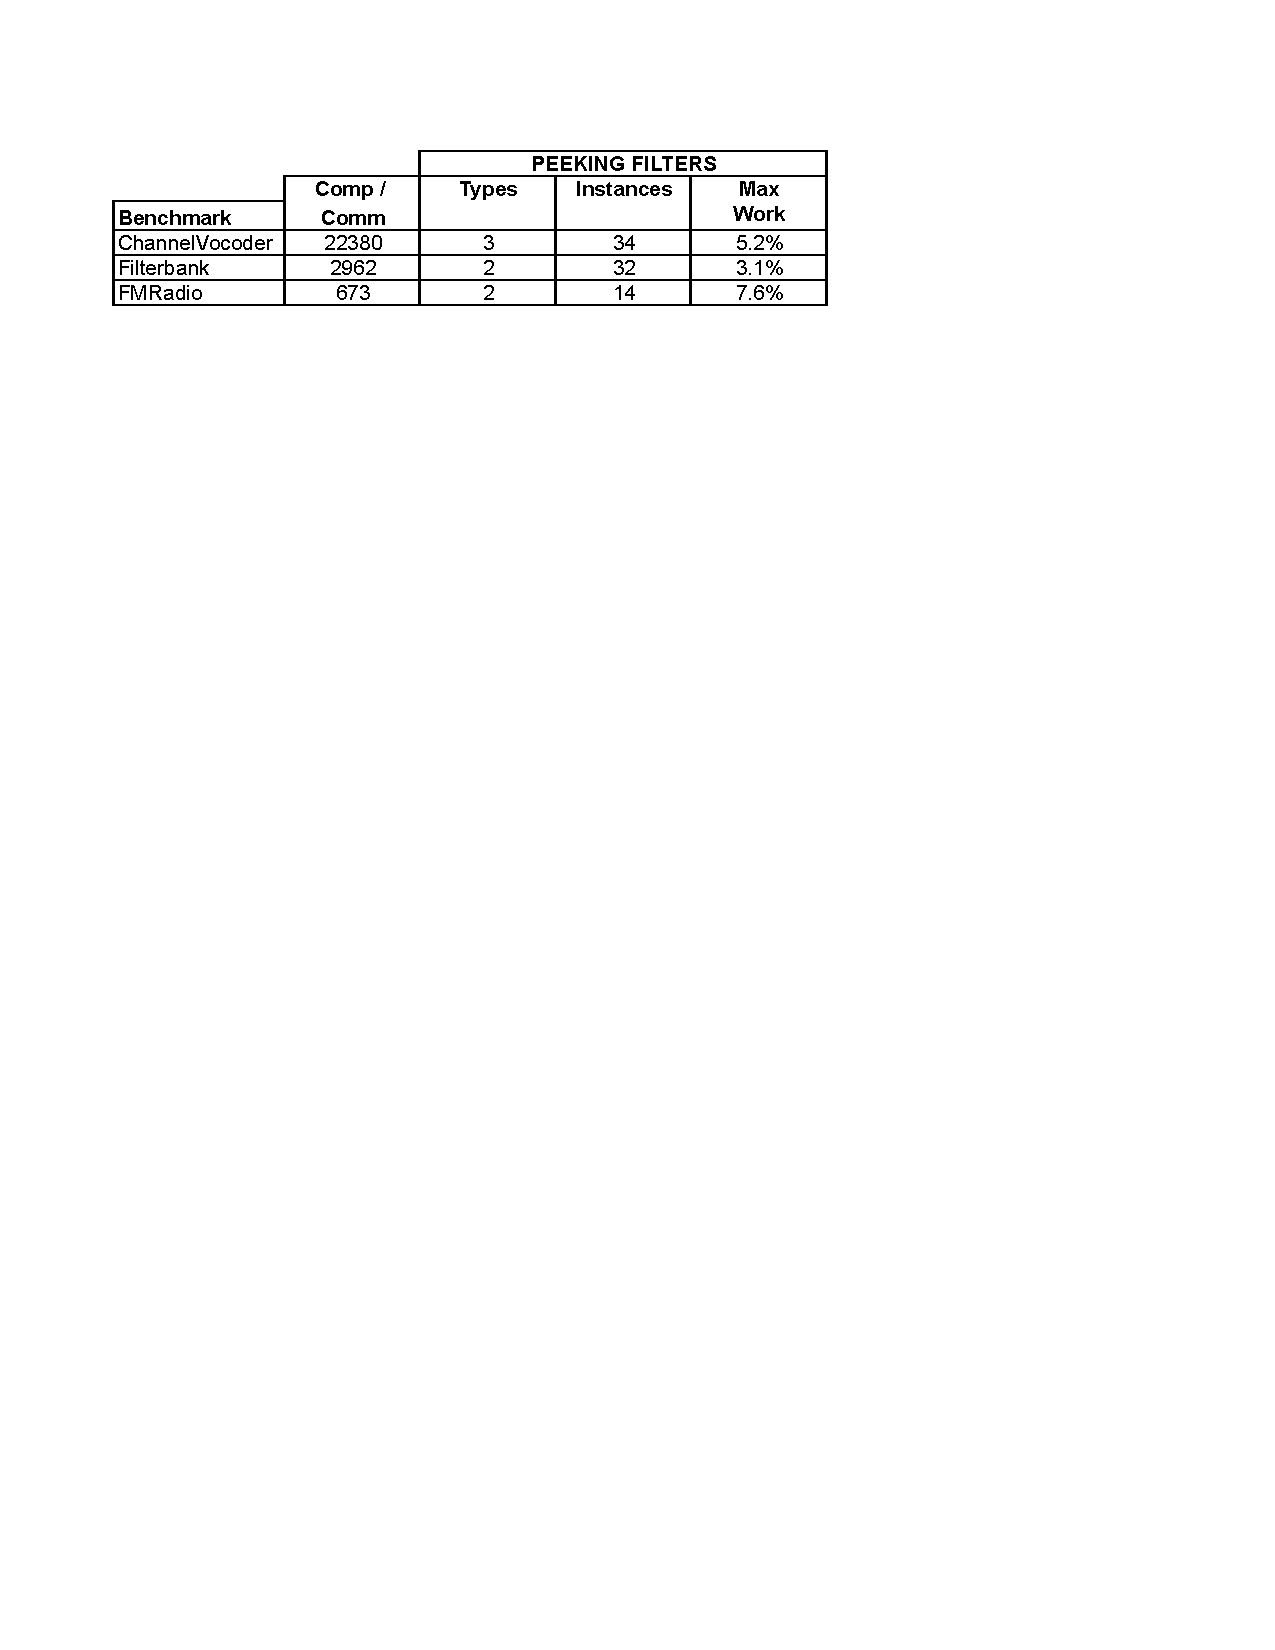
\includegraphics[width=3.3in]{figures/bench-char.pdf}}

\noindent ``Comp/Comm'' provides a static estimation of the
amount of computation to communication ratio by statically estimating the total
work of all the filters and dividing by the number items communicated
for the programmer-conceived graph's steady-state.  The remaining
statistics give the number of peeking filters types, number of peeking
filters instantiated at runtime, and a static estimation of the maximum
work in the single most loaded peeking filter.

We target 2 multicore architecture with different communication
mechanisms.  The Tilera Corporation's TILE64 Processor is a 64 core
system on a chip~\cite{tilera}.  Each core is an identical three-wide
VLIW. The code generated by the StreamIt
compiler for the TILE64 processor follows the remote store programming
(RSP) model~\cite{rsp10} in which each process has a private address
space, but each process can award remote processes write access to
their local memory. When a producer process has write access to a
consumer process's memory, the producer communicates directly with the
consumer via store instructions whose destination is an address in the
consumer's shared memory.  Communication is initiated by the producer,
and is fine-grained.  The consumer reads directly from it's local
memory (L2) when accessing input.

Our symmetric multiprocessor target is a 16-core architecture that is
comprised of four Intel Xeon E7350 multicore processors.  Each processor
is a 64-bit, quad-core with two dual-core dies.  Each die contains a 4
MB L2 cache shared across the two cores.  The front-side bus is clocked
at 1066 MHz.  We utilize the cache coherency mechanism of the
architecture for communication between cores. 

Through empirical experimentation on FMRadio, Filterbank, and
ChannelVocoder, we have settled on $T_{\mt{sharing}} =.10$ and
$T_{\mt{apply}} = 0.05$. These constants are the sweet stop for the two
architectures employed in the experimentation, being a good compromise
between buffer size and inter-core communication.

% \begin{figure*}[t]
% \centering
% \subfigure[]{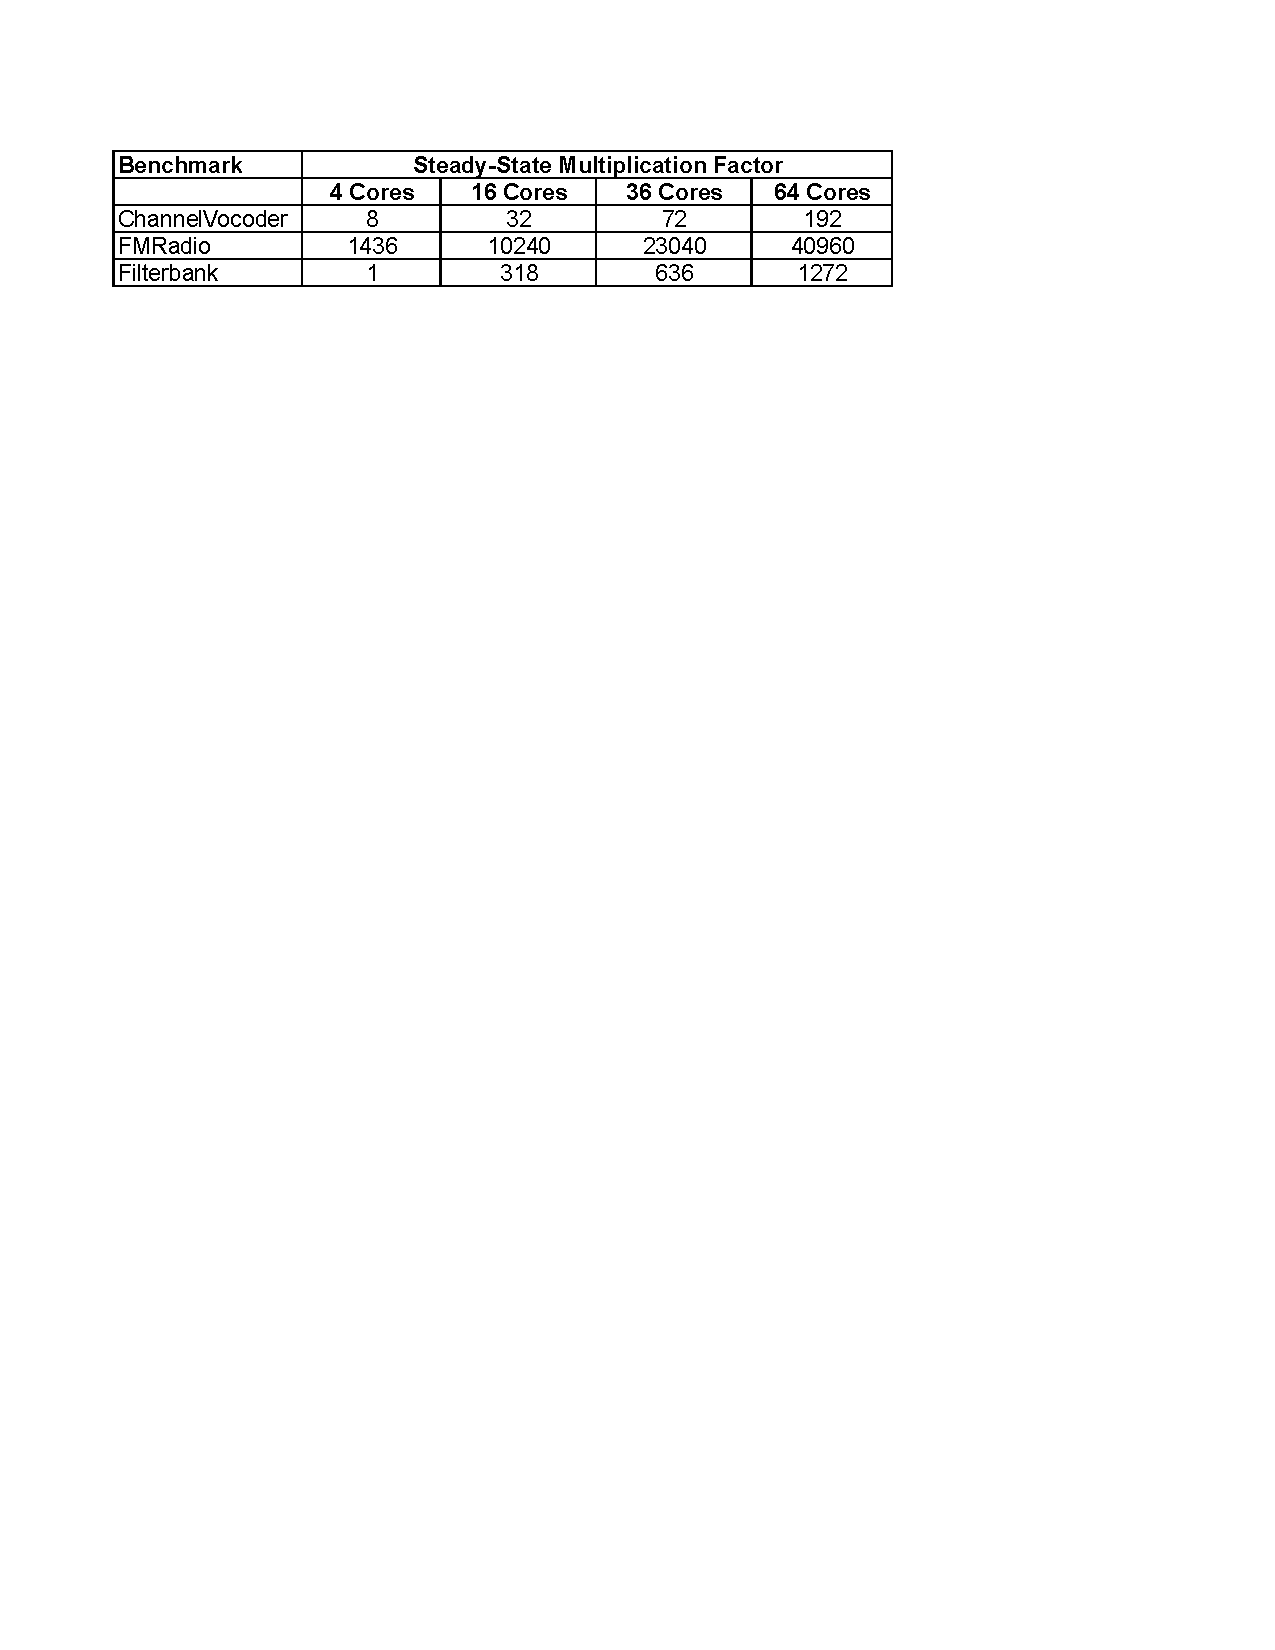
\includegraphics[width=3.7in]{figures/mult-table.pdf}} \\
% \subfigure[]{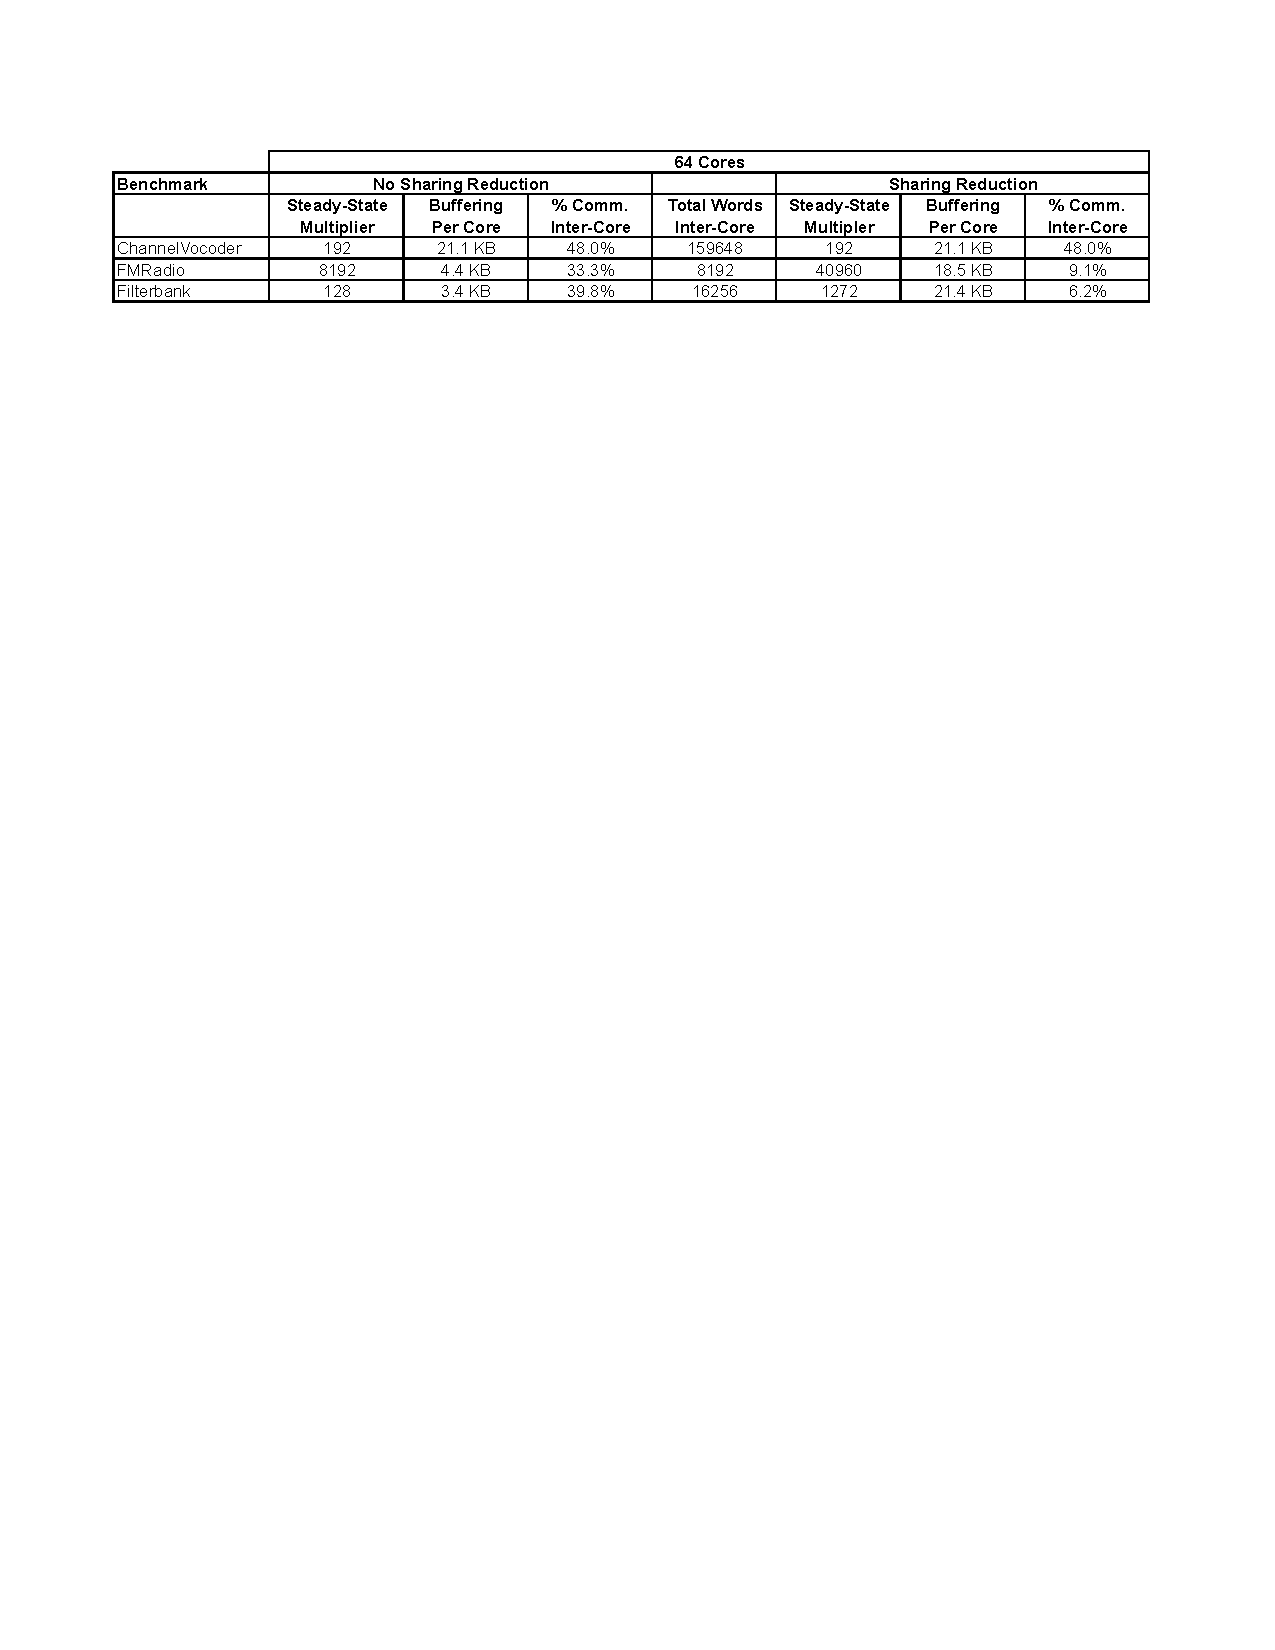
\includegraphics[width=6in]{figures/64-core-table.pdf}}
% \caption[Communication, multiplier and buffering statistics for
% benchmarks.]{
% Communication, multiplier and buffering characteristics for
% benchmarks: (a) gives the steady-state multipliers calculated for
% sharing reduction, (b) compares the steady-state with and without
% sharing reduction. 
% \label{fig:fission-table}}
% \end{figure*}

\begin{figure*}[t]
\centering
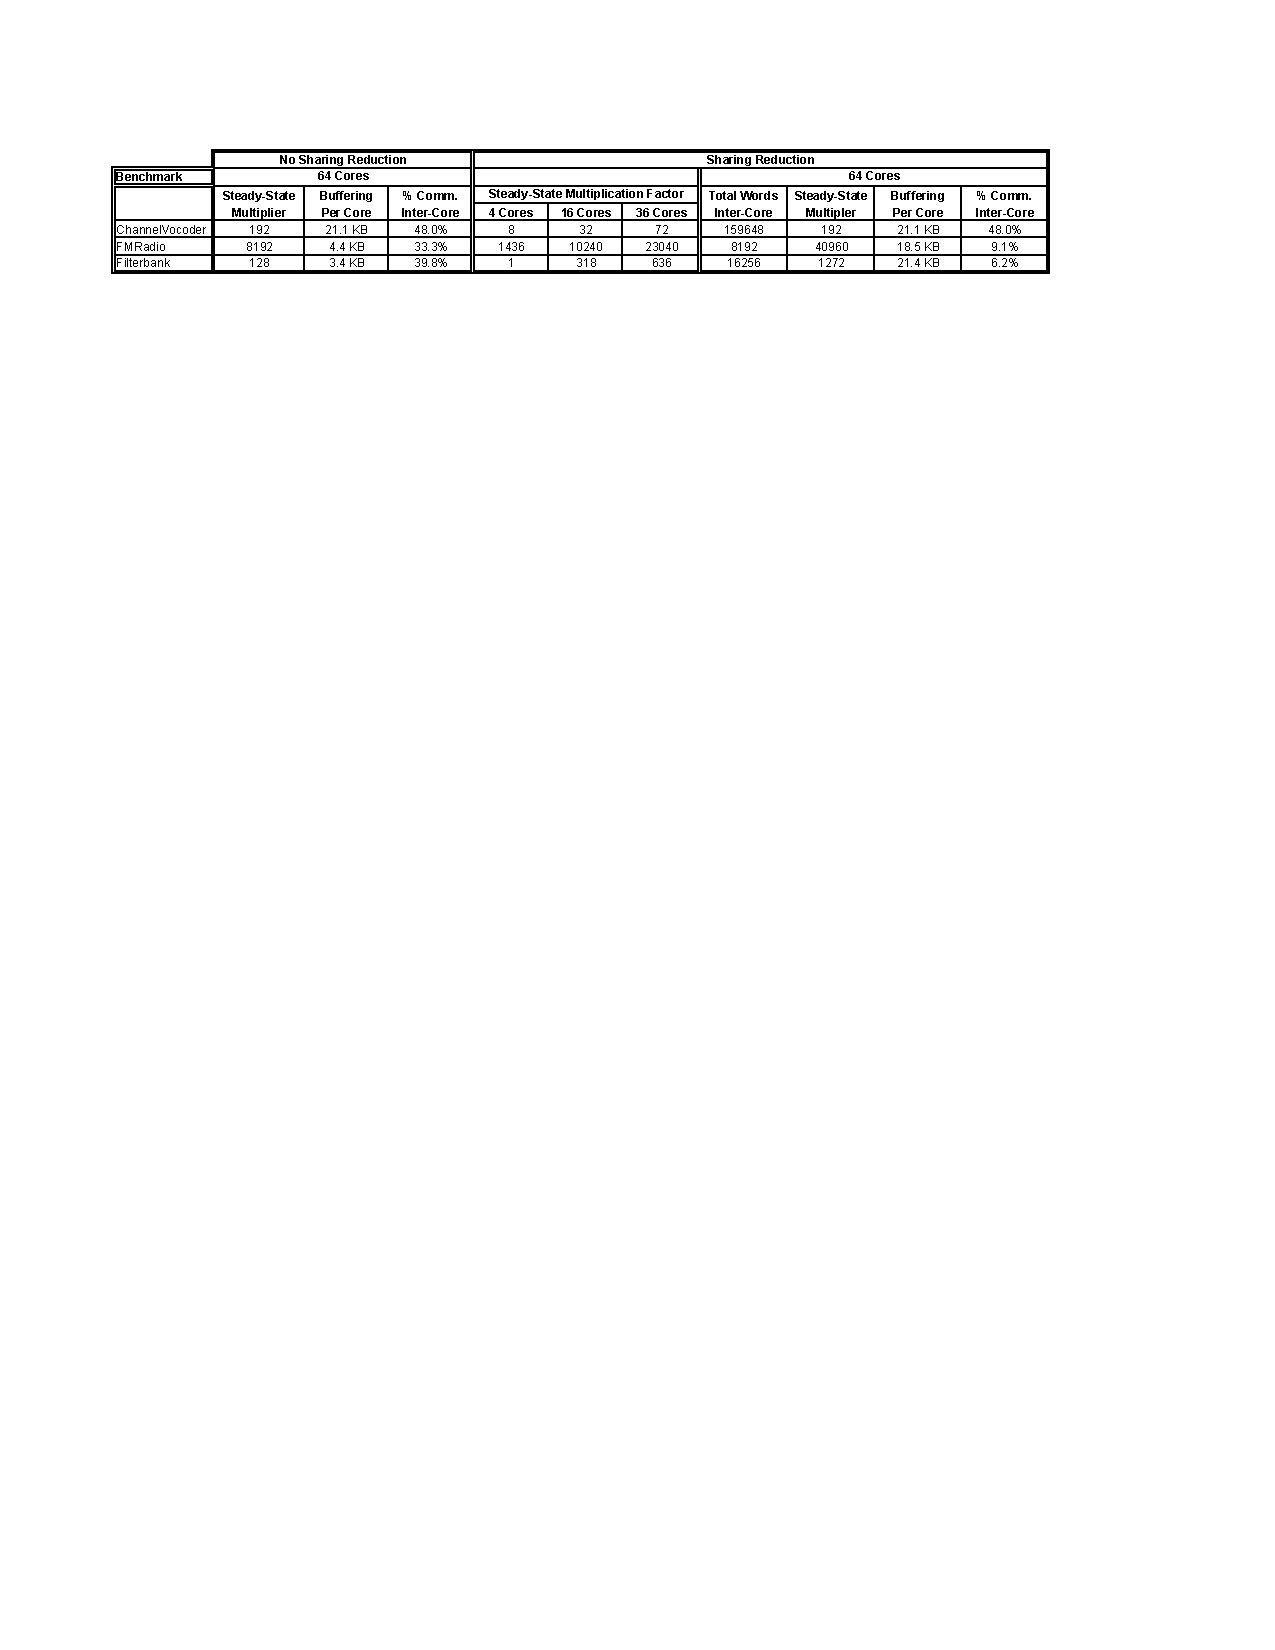
\includegraphics[width=6.1in]{figures/big-table.pdf}
\caption{\label{fig:big-table}  Steady-state multiplicity, buffering,
  and communication for fission with and without sharing reduction.}
\end{figure*}

% \begin{figure}[t]
% \centering
% 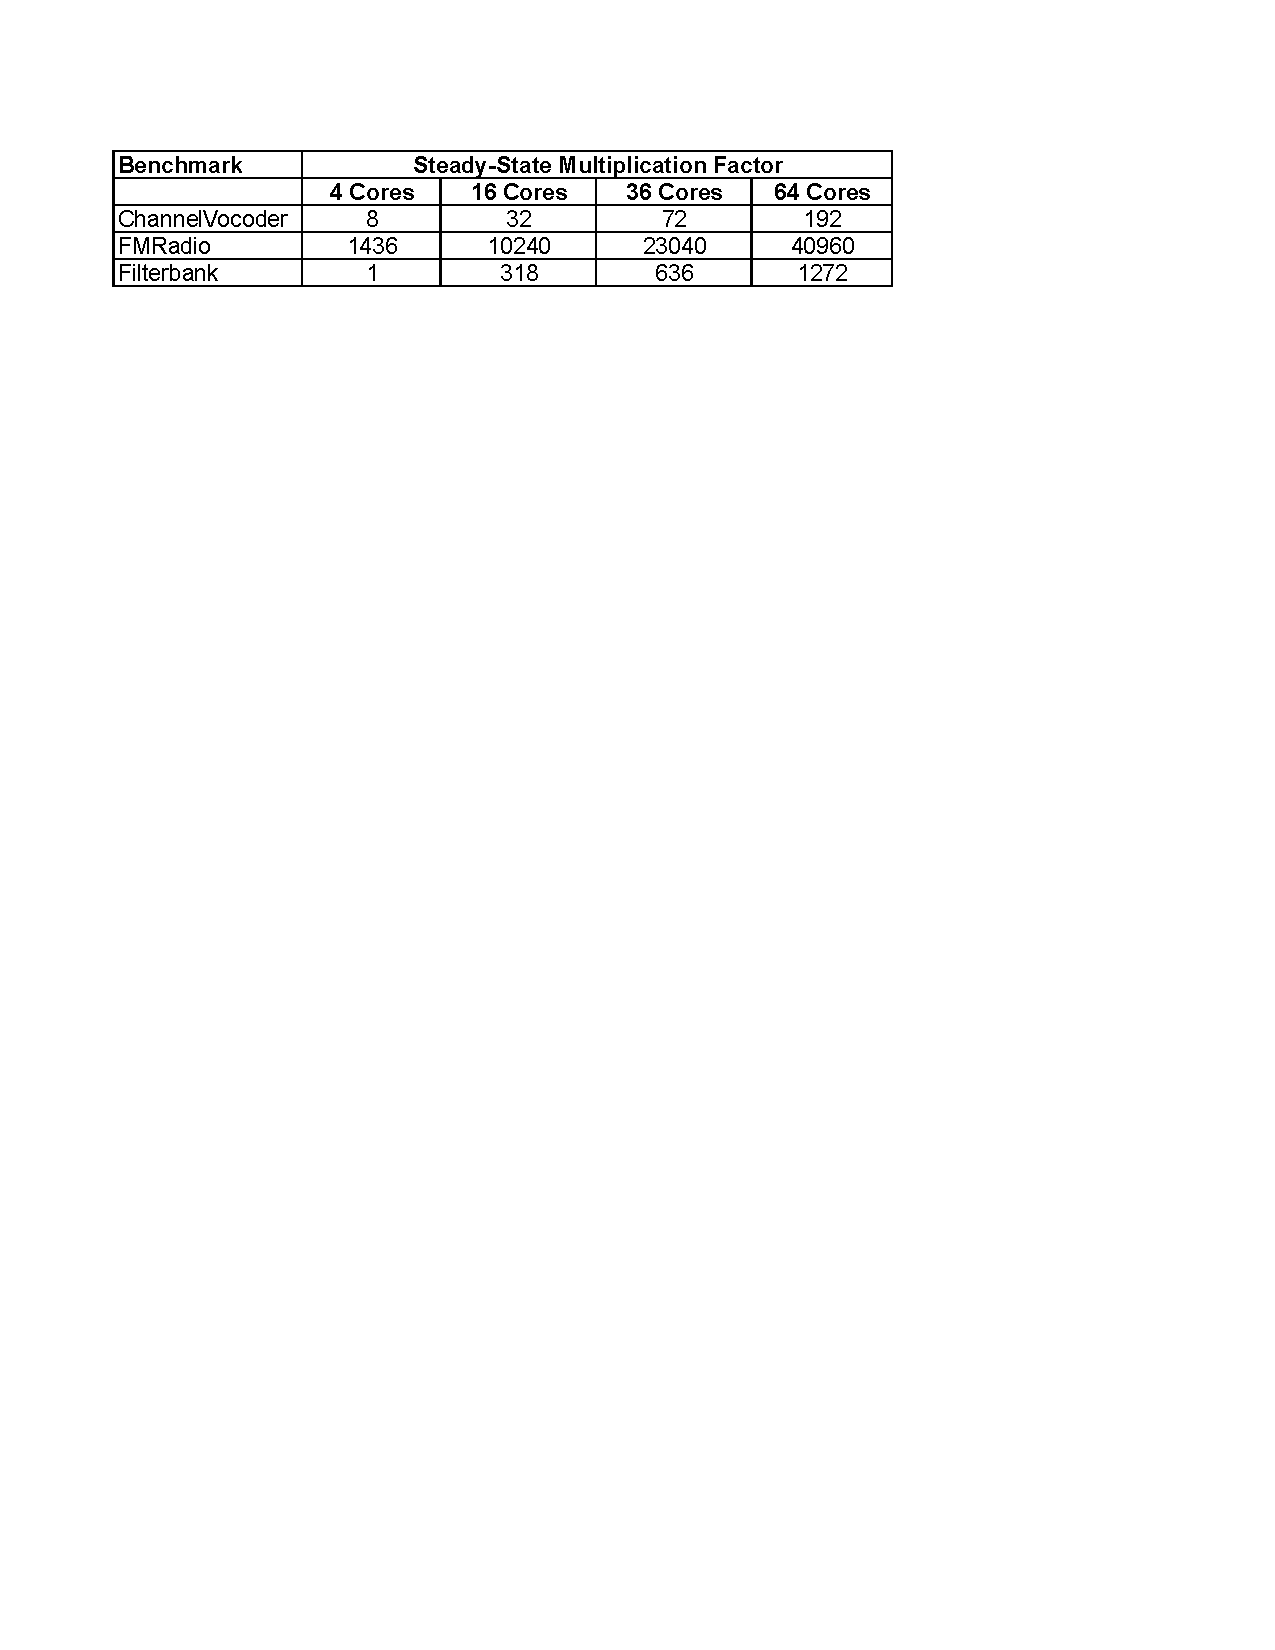
\includegraphics[width=3.3in]{figures/mult-table.pdf}
% \caption{\label{fig:mult-table}  The steady-state multipliers calculated for
% sharing reduction.}
% \end{figure}

% \begin{figure*}[t]
% \centering
% 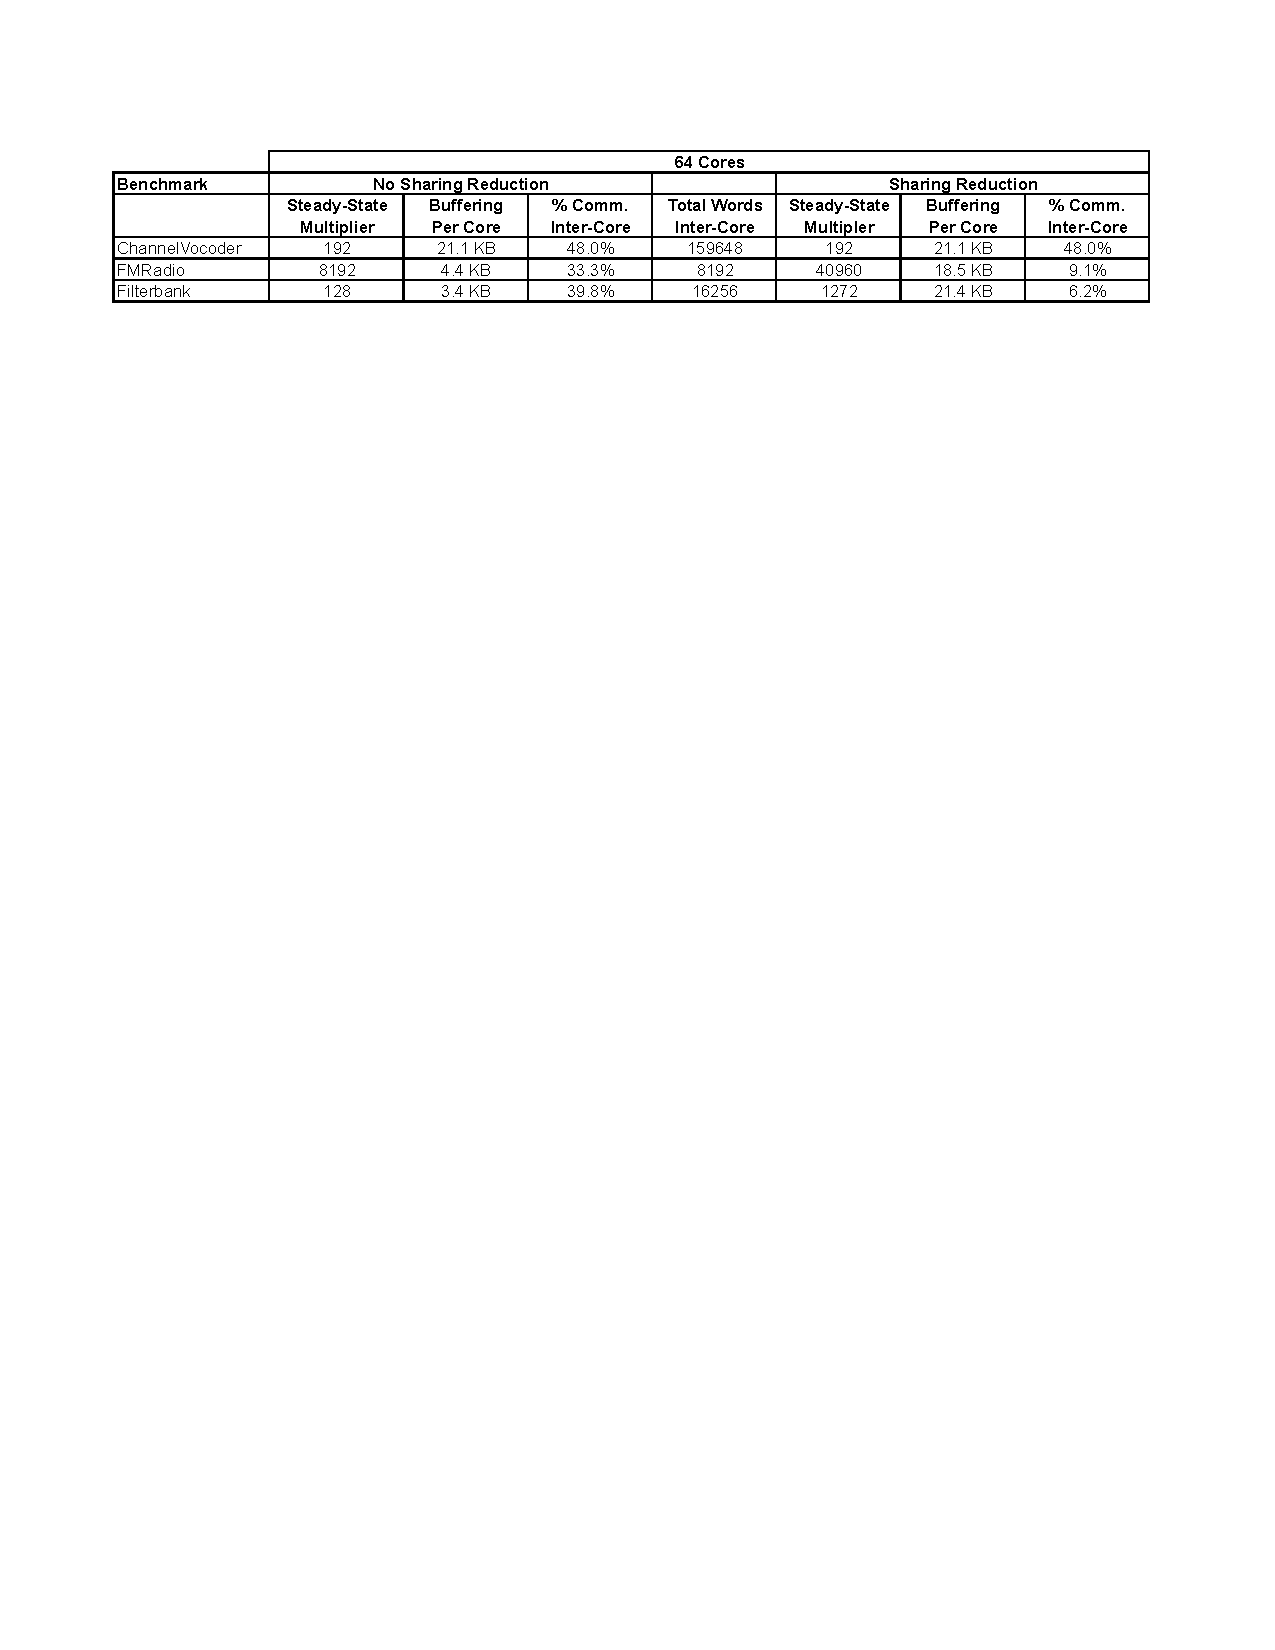
\includegraphics[width=6in]{figures/64-core-table.pdf}
% \caption{ Multiplier, buffering and communication for the steady-state with and without
% sharing reduction. 
% \label{fig:fission-table}}
% \end{figure*}

Figure~\ref{fig:big-table} compares the steady-state with and
without sharing reduction for a 64-core mapping, as well as gives the
constant $c$ calculated by sharing reduction for 4, 16, and 36.  The
factor is larger for FMRadio because one filter has $C(f) \gg o(S,
f)$.  The multiplication factor affects both latency and buffer sizes
adversely.  The application designer will have to decide if the
latency of these techniques can be borne given the application
criteria.  The total buffering requirement is increased when the
steady-state is increased.  However, since we are then fissing, the
buffer is divided amongst the fission products, and the {\it per-core}
buffering requirement is unaffected by the increase.  For example,
FMRadio, has a per-core 18 KB buffering requirement across all
configurations (4, 16, 36, and 64 cores).  This requirement fits in
the per-core L2 size of 64 KB for the Tile64.

 For ChannelVocoder,
sharing reduction has no effect because most of the peeking filters do
not satisfy $T_{\mt{apply}} = 0.05$ because of differing fission
factors between producers and consumers.  For the peeking filters that do,
the steady-state multiplier required for legal general fission for the
graph is enough to assure $T_{\mt{sharing}}$ is met.  Even though
sharing reduction has no effect for ChannelVocoder, general fission
avoids the 38\% of total items that were unnecessary duplicated by
DupDec.

For FMRadio and Filterbank, sharing reduction leads to significant
decreases in the percentage of total items communicated inter-core for
each steady-state.  The buffer requirement is increased an average of
5.2x for these benchmarks.  The total number of words communicated
inter-core during each steady-state is the same, with and without
sharing reduction.  However, the steady-state is greater in the
sharing reduction case, thus producing more outputs.

\begin{figure}[t]
\centering
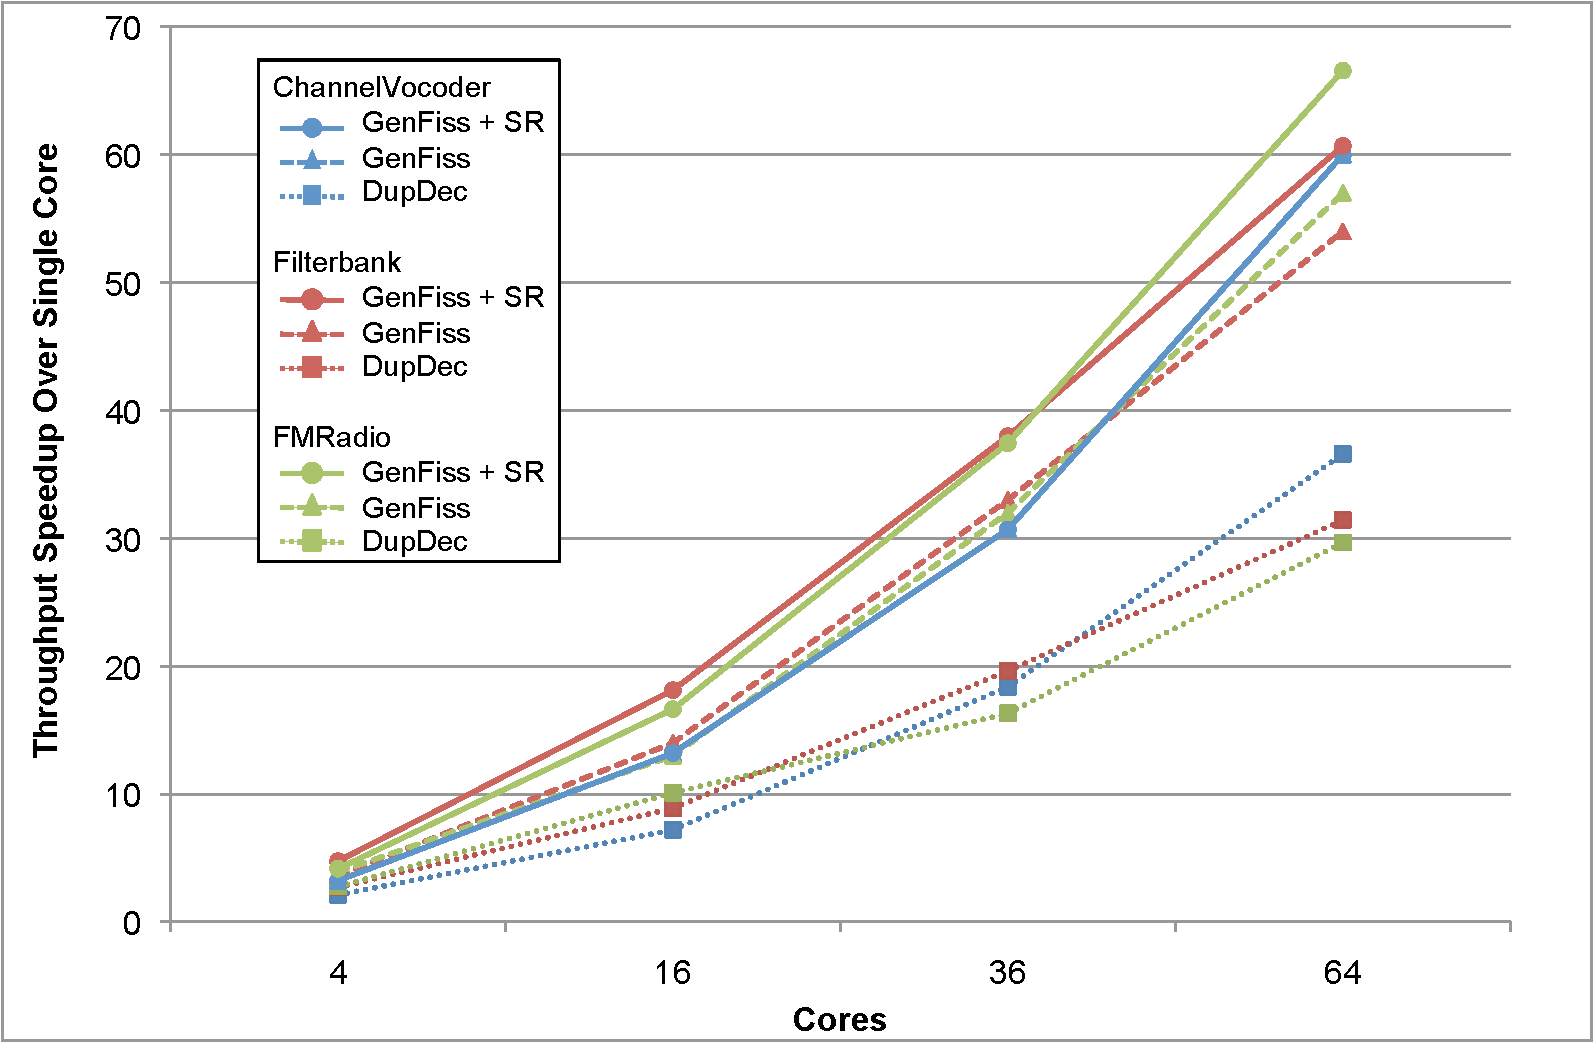
\includegraphics[width=3.3in]{figures/tilera-chart.pdf}
\caption[Comparing the fission techniques on the TILE64.]{
  Evaluation for DupDec versus general fission versus general fission with sharing reduction
  4, 16, 36, and 64 cores on the TILE64.  \label{fig:tilera-chart}}
\end{figure}

Figure~\ref{fig:tilera-chart} gives the performance results for the
Tilera TILE64 architecture.  We present results for DupDec, general
fission, and general fission with sharing reduction for 4, 16, 36, and
64 core configurations, with throughput normalized to single-core
throughput.  General fission with sharing reduction outperforms
DupDec by an average of 1.8x for the three benchmarks when targeting
64 cores. The average 64-core speedup over single core is 62.3x for the
general fission plus sharing reduction for these three benchmarks.

FMRadio experiences the most significant gain from general fission
plus sharing reduction over DupDec (67x versus 30x, respectively, for
64 cores).  FMRadio has the lowest computation to communication ratio
of the 3 benchmarks.  Furthermore, each filter of is fissed by the
number of cores targeted.  For 64 cores, each filter is fissed 64
ways.  DupDec must perform a global all-to-all communication involving
all 64 cores between each level of the graph!
 
ChannelVocoder achieves a 60x speedup for general fission over a
single core.  This is not perfectly linear because of the parallel
mapping; asymmetries exist between the extent of task parallelism and
the number of cores (see~\ref{mgordon-asplos06}).  The speedup over
DupDec (1.62x) is more modest because the width of many of the
fission applications is 3, so DupDec is duplicating input data to
groups of 3 filters.  Filterbank is similar, the width of fission is 4
for all filters when targeting 64 cores.

Sharing reduction is required to achieve scalable speedups for both
FMRadio and Filterbank.  For FMRadio, sharing reductions leads to a
17\% speedup increase for 64 cores.  This because sharing reduction
significantly reduces the number of remote write store instructions
required per output.  This affects FMRadio because of its low
computation to communication ratio.  Sharing reduction sees a 12\%
increase on Filterbank, as Filterbank has a larger computation to
communication ratio.

\begin{figure}[t]
\centering
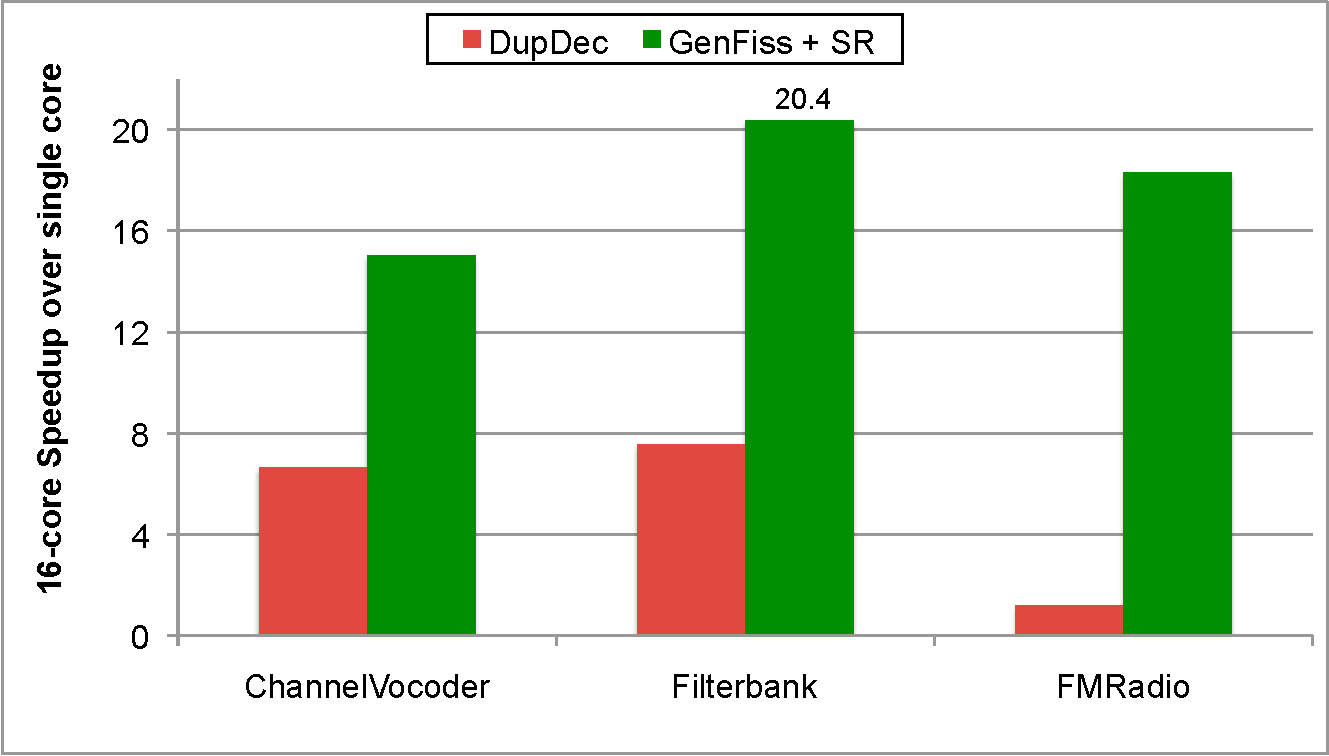
\includegraphics[width=3.3in]{figures/smp-chart.pdf}
\caption[Comparing the fission techniques on the 16-core SMP.]{
  Evaluation for DupDec versus general fission with sharing reduction
  for the 16-core SMP architecture.  \label{fig:smp-chart}}
\end{figure}

Our techniques enable scalable parallelization, with a mean speedup of
17x for our 3 benchmarks on the SMP.  Figure~\ref{fig:smp-chart} gives
the 16-core speedup comparison for DupDec versus general fission with
sharing reduction for our target SMP architecture.  The mean speedup
increase for general fission with sharing reduction over DupDec is
6.7x.  FMRadio again sees the largest speedup increase in the
comparison at 13.0x.  The reasons for this large speedup are similar
as given in the previous section.  However, the SMP communication
mechanism is not as efficient as the TILE64, thus general fission with
sharing reduction gives a greater speedup because reducing inter-core
communication has more impact.

  \section{Related Work}
\label{sec:related}

% BILL

%Signal~\cite{Signal}, 
%Lucid~\cite{Lucid77}, and
%Occam~\cite{Occam}, and Sisal \cite{sisal}.
%Parallel Haskell~\cite{ph}
In addition to StreamIt, there are a number of stream-oriented
languages drawing from domains such as functional, dataflow, CSP and
synchronous programming~\cite{survey97}.  The Brook language is
architecture-independent and focusses on data
parallelism~\cite{brook04}.  Stream kernels are required to be
stateless, though there is special support for reducing streams to a
single value.  Stream\-C/Ker\-nel\-C is lower level than Brook;
kernels written in KernelC are stiched together in StreamC and mapped
to the data-parallel Imagine processor~\cite{imagine03ieee}.  SPUR
adopts a similar decomposition between ``microcode'' stream kernels
and skeleton programs to expose data parallelism~\cite{spur05samos}.
Cg exploits pipeline parallelism and data parallelism, though the
programmer must write algorithms to exactly match the two pipeline
stages of a graphics processor~\cite{cg03}.  Compared to these
languages, StreamIt places more emphasis on exposing task and pipeline
parallelism (all the languages expose data parallelim).
%and on sliding window operations (filters that peek).  
By adopting the synchronous dataflow model of execution~\cite{lee87},
StreamIt focusses on well-structured programs that can be aggressively
optimized.  The implicit infinite loop around programs is also a key
StreamIt characteristic that enables the transformations in this
paper.  Spidle is also a recent stream language that was influenced by
StreamIt~\cite{spidle03}.
%and Lucid Synchrone~\cite{Lucid-Synchrone}.
%Synchronous languages which
%target embedded applications include Esterel~\cite{Esterel},
%Lustre~\cite{Lustre}, and Additional

Liao et al. map Brook to multicore processors by leveraging the affine
partitioning model~\cite{liao06brook}.  While affine partitioning is a
powerful model for parameterized loop-based programs, in StreamIt we
simplify the problem by fully resolving the program structure at
compile time.  This allows us to schedule a single steady state using
flexible, non-affine techniques (e.g., simulated annealing) and to
repeat the found schedule for an indefinite period at runtime.
Gummaraju and Rosenblum map stream programs to a general-purpose
hyperthreaded processor~\cite{gummaraju05micro}.  Such techniques
could be integrated with our spatial partitioning to optimize per-core
performance.  Gu et al. expose data and pipeline parallelism in a
Java-like language and use a compiler analysis to efficiently extract
coarse-grained filter boundaries~\cite{du03sc}.  Ottoni et al. also
extract decoupled threads from sequential code, using hardware-based
software pipelining to distribute the resulting threads across
cores~\cite{ottoni05decoupled}.  By embedding pipeline-parallel
filters in the programming model, we focus on the mapping step.

%%%%%%%%%%%%%%%%%%%%%%%%%%%%%%%%%%%%%%%%%%%%%%%%%%%%%%%%%%%%%%%%%%%%%

Previous work in scheduling computation graphs to parallel targets has
focused on partitioning and scheduling techniques that exploit task
and pipeline parallelism~\cite{SDFSched, SDFSched2,may87communicating,
DAGSched, pipeline-sdf}.  Application of loop-conscious
transformations to coarse-grained dataflow graphs has been
investigated.  Unrolling (or ``unfolding'' in this domain) is employed
for synchronous dataflow (SDF) graphs to reduce the initiation
interval but they do not evaluate mappings to actual
architectures~\cite{unfolding,unfolding2}. Software pipelining
techniques have been applied to SDF graphs onto various embedded and
DSP targets~\cite{bakshi99,chatha-02}, but has required programmer
knowledge of both the application and the architecture. To our
knowledge, none of these systems automatically exploit the combination
of task, data, and pipeline parallelism.  Furthermore, these systems
do not provide a robust end-to-end path for application
parallelization from a high-level, portable programming language.

%% Previous work on instruction-level software pipelining has focused
%% mostly on scheduling machine instructions in a loop via modulo
%% scheduling~\cite{rau81,lam-softpipe}.  The algorithms devised must
%% account for tight resource constraints and complex instruction
%% dependences. Our software-pipelining problem is much less constrained,
%% enabling us to employ a simple greedy heuristic.  

%% Furthermore, a traditional modulo scheduling algorithm is not needed
%% because we have an implicit loop barrier at the end of each
%% steady-state.  ILP compilers for clustered VLIW
%% architectures~\cite{Bulldog,Multiflow,lee98spacetime,qian02} must
%% partition instructions and assign them to clusters as part of the
%% instruction scheduling. Clustering is analogous to our application of
%% filter fusion in our software pipelining algorithm.

  \section{Conclusion}
\label{sec:conclusion}

In this paper, we describe the StreamIt compiler for the Raw
architecture.  The stream graph of a StreamIt program exposes the data
communication pattern to the compiler while the lack of global
synchronization frees the compiler to radically reoganize the program
for efficient execution on the underline architecture. The StreamIt
compiler demonstrates the power of this flexibility by totally
reoganizing large programs for better load balance. We were able to
map many of programs on to the Raw processor and obtain good
performance.

We introduce a collection of optimizations, vertical and horizontal
filter fusion, vertical and horizontal filter fission and filter
reordering transformations, that can be used to restructure stream
graphs.  We show that by applying these transformations we can map a
high-level stream program, written to reflect the composition of the
application, onto Raw and achieve good processor utilization and load
balance, leading to a factor of three speedup on two applications.

Unlike all previous streaming languages, the structured streams of
StreamIt makes it possible for us to approach the optimization and
parallelization problems in a very systermatic manner. It enables us
to define multiple optimizations -- targetting different constructs
and requirements -- and to compose them them in a hirearchical manner.

The ability to do global transformations across multiple filters, that
may have originated from very different parts of the application,
makes it possible for the compiler to find optimization opportunities
that may ellude even an experience programmer.  Such capabilities
enables the programmers to write protable streaming applications and
map them efficiently onto any given architecture. This has the
potential of creating a programming standard for emerging
communication exposed architectures.  The StreamIt compiler takes a
fist step towards this goal.


  %\section{Precise Event Handling}
In this section we describe how $\sdep$ information can be
incorporated into the semantics of a language feature that provides
precise delivery of control messages in stream programs.  Our goal is
to improve both programmer productivity and performance.

The Synchronous Dataflow (SDF) domain is well-suited for applications
that have regular, high-bandwidth communication patterns.  However, in
realistic streaming applications there are also irregular,
low-bandwidth control messages that are used to adjust parameters in
various parts of the stream.  For example, a downstream actor might
detect a high signal-to-noise ratio and send a message to the
communications frontend to increase the amplification.  Or, an actor
at the top of the stream graph might detect an invalid checksum for a
packet, and send a message downstream to invalidate the effects of
what has been processed.  Other examples of control messages include:
periodic channel characterization; adaptive beamforming; initiating a
handoff ({\it e.g.,} to a new network protocol); marking the end of a
large data segment; and responding to user inputs, environmental
conditions, or exceptional states.

Generally speaking, control messages are sent at infrequent and
irregular intervals; however, once they are generated there might be
tight constraints on their delivery.  For example, the message
invalidating the effects of a given packet has to be delivered exactly
in sync with the front of the packet itself; otherwise, valid data
will be lost or invalid data will be allowed to pass.

In the rest of this section, we describe language support for control
messages that makes use of $\sdep$ to achieve precise delivery timing.
We first describe the semantics of the language feature, and then we
compare it against other means of implementing messages for a
frequency hopping radio application.

\subsection{Messaging with SDEP}

The messaging system we describe is included as part of the StreamIt
language~\cite{streamitcc}.  In StreamIt, there are two distinct kinds
of communication between filters during steady state execution: 1)
high-bandwidth dataflow over the FIFO channels in the graph, and 2)
low-bandwidth messaging between pairs of filters\footnote{Messaging
is possible whenever there is a downstream path from either filter to
the other.  Filters running in parallel cannot send messages}.  In
order for filter $A$ to send a message to filter $B$, the following
steps need to be taken:
\begin{itemize}

\item $B$ declares a message handler that will be invoked when the
message arrives, for example:
{\small
\begin{verbatim}
handler increaseGain(float amount) {
  this.gain += amount;
}
\end{verbatim}
}
Message handlers are just like normal functions, except that they
cannot access the input/output channels and they have no return value.

\item A parent stream which contains $A$ and $B$ declares a variable
of type {\tt portal<} $T_B$ {\tt >} which can forward messages to
anything of type $T_B$.  The parent adds $B$ to the portal and passes
the portal to $A$ during initialization.

\item To send a message, $A$ invokes the handler method on the portal
from within its steady state work function.  It includes a range of
latencies at which the message should be delivered.  For example:
{\small
\begin{verbatim}
work pop 1 {
  float val = pop();
  if (val < THRESHOLD) {
    portalToB.increaseGain(0.1) [2:3];
  }
}
\end{verbatim}}

\end{itemize}
The most interesting aspect of the messaging system is the semantics
for message latency.  Because there are many legal orderings of actor
executions, there is no notion of ``global time'' in a stream graph.
The only common frame of reference between concurrently executing
actors is the series of data items that is passed between them.  The
$\sdep$ function captures the data dependences in the graph and
provides a natural means of defining a rendezvous point between two
actors.

Intuitively, the message semantics can be thought of in terms of
attaching tags to data items.  If $A$ sends a message to downstream
filter $B$ with a latency $k$, then this could be implemented by
tagging the items that $A$ outputs $k$ iterations later.  These tags
propagate through the stream graph; whenever an actor inputs an item
that is tagged, all of its subsequent outputs are tagged.  Then, the
message handler of $B$ is invoked immediately after the first
invocation of $B$ that inputs a tagged item.  In this sense, the
message has the semantics of traveling ``with the data'' through the
stream graph, even though it does not have to be implemented this way.

The intuition for upstream messages is similar.  Consider that $B$ is
sending a message with latency $k$ to upstream actor $A$ in the stream
graph.  This means that $A$ will receive the message immediately
following the last invocation of its work function which produces an
item affecting the output of $B$'s $k$th firing, counting the current
firing as 0.  As before, we can also think of this in terms of $A$
tagging items and $B$ observing the tags.  In this case, the latency
constraint says that $B$ must input a tagged item before it finishes
$k$ additional executions.  The message is delivered immediately
following the latest firing in $A$ during which tagging could start
without violating this constraint.

The following definition leverages the $\sdep$ formalism to give a
precise meaning to message timing.

\begin{definition}(Message delivery)
Consider that $A$ sends a message to $B$ with latency range
$[k_1:k_2]$ and that the message is sent during the $n$th invocation
of $A$'s work function.  Then the message handler can be invoked in
$B$ immediately after its work function has fired ${\cal M}(A, B, k_1,
k_2, n)$ times, where ${\cal M}$ is constrained as follows.

There are two cases\footnote{In a feedback path, both cases might apply.  In this event, we assume the message is being sent upstream.}:
\begin{enumerate}

\item There is a path in the stream graph from $A$ to $B$.  Then
${\cal M}$ obeys the following constraints:
\[
\begin{array}{l}
\sdepf{A}{B}({\cal M}(A, B, k_1, k_2, n)) \ge n+k_1\\
\sdepf{A}{B}({\cal M}(A, B, k_1, k_2, n)) \le n+k_2
\end{array}
\]

\item There is a path in the stream graph from $B$ to $A$.  Then
${\cal M}$ obeys the following constraints:
\[
\begin{array}{l}
{\cal M}(A, B, k_1, k_2, n) \ge \sdepf{A}{B}(n + k_1)\\
{\cal M}(A, B, k_1, k_2, n) \le \sdepf{A}{B}(n + k_2)
\end{array}
\]
\end{enumerate}
\end{definition}

\begin{table*}[t]
{\small
\begin{tabular}{|r|c|c|} \hline
~ & {\bf Negative latency} & {\bf Positive latency} \\ \hline
{\bf Message travels downstream} & latency in schedule must not be too small & no constraint \\ \hline
{\bf Message travels upstream} & impossible & latency in schedule must not be too big \\ \hline
\end{tabular}}
\caption{\small Effect of message direction and latency on stream graph execution.}
\label{tab:messcons}
\end{table*}

It is instructive to note that there are distinct categories of
message latencies, each of which poses a different constraint on the
execution of the stream graph (see Figure~\ref{tab:messcons}).  A
negative-latency downstream message has the effect of synchronizing
the arrival of the message with some data that was previously output
by the sender ({\it e.g.,} for the checksum example used above).  The
latency requires the downstream actor not to execute too far ahead, or
else it might process the data before the message arrives.  This
translates to a constraint on the minimum latency between the sender
and receiver actors in the schedule of the program.

Similarly, a positive latency upstream message places a constraint on
the maximum latency between the sender and receiver.  Again the
receiver must be throttled so that it doesn't get too far ahead before
the message arrives; however, because the receiver is upstream of the
sender, this constraint represents the need for a tight coupling
between the two filters' executions.

An upstream message with negative latency is impossible to deliver,
because the data dependences imply that the target iteration has
already passed when the message was sent.  Also, a downstream message
with positive latency imposes no constraint, as it is not possible for
the receiver to have executed yet.

\begin{figure}[t]
\begin{center}
\psfig{figure=constrained-example.eps,height=1.5in}
\caption{{\small Example of construction of a constrained schedule. The $\sdepf{R}{S}$ function for filters $R$ and $S$ is given in Table \ref{tab:sdepconst}. The blob between filters $R$ and $S$ illustrates other possible stream elements. $R$ sends a message to $S$ with latency $[1,2]$. Executions of the blob are omitted, it is assumed that at the point $S$ executes, the blob has drained data provided by $R$.}}
\end{center}
\vspace{-12pt}
\label{fig:sdepconst}
\end{figure}

\begin{table*}[t]
{\small
\begin{tabular}{|c|c|} \hline
{\bf $sdepf{R}{S}$} & {\bf Execs of S} \\ \hline
$9n+2$ & $8n+1$ \\ \hline
$9n+3$ & $8n+2$ \\ \hline
$9n+5$ & $8n+3$ \\ \hline
$9n+5$ & $8n+4$ \\ \hline
$9n+6$ & $8n+5$ \\ \hline
$9n+8$ & $8n+6$ \\ \hline
$9n+9$ & $8n+7$ \\ \hline
$9n+9$ & $8n+8$ \\ \hline
\end{tabular}}
\caption{\small $sdepf{R}{S}$ function for example in Figure \ref{fig:sdepconst}. This particular $\sdep$ function was obtained by setting $push_R=2$, $pop_S=3$ and making the blob between $R$ and $S$ into a filter that pops 3 and pushes 4 every iteration of its work function. No initialization due to peeking is necessary in this example.}
\label{tab:sdepconst}
\end{table*}


Explanation of working of the example:

The example in Figure \ref{fig:sdepconst} illustrates scheduling of a single constraint. The constraint is a message sent upstream with latency $[1,2]$. The resulting schedule consists of two parts, an initialization schedule and a steady state schedule. The initialization schedule is necessary to initialize the constraint, to ensure that the steady schedule can be executed repeatedly forever. Notation used here is: $lastReceived$ denotes the execution of S which sent the last message to be received by R; $n_S$ indicates number of executions of $S$ and $n_R$ indicates number of executions of $R$.

Initialization schedule is computed by executing R $SDEP(minLatency)-1$ number of times, and executing S as many times as possible, given data provided by R. This assures that when the steady schedule starts, all executions of filters will contribute to new message sending and receiving, thus allowing the steady state schedule to execute forever. The initialization schedule does not need to send or receive messages here.

The steady state schedule is computed by executing the receiver R as far as possible without going beyond the boundary of being able to receive message sent by S on execution $lastReceived+1$ (indicated by "Oldest msg to receive" in the figure). Now the sender S is executed as many times as possible, given data provided by R. Now S can receive messages sent by S in its executions $[lastReceived+1 ... \min(n_S, $"Newest msg to receive"$)]$.

"Oldest msg to receive" is equal to $iSDEP(n_R)-maxLatency$. "Newest msg to receive" is equal to $m-minLatency$ with $m$ being the greatest integer such that $SDEP(m) \le n_R$.


\subsection{Case Study}

To illustrate the pros and cons of the messaging system, we
implemented a spread-spectrum frequency hopping radio
frontend~\cite{harada02} as appears in Figure~\ref{fig:fhr-streamit}.
A frequency hopping radio is one in which the receiver switches
between a set of known frequencies whenever it hears certain tones
from the transmitter.  The frequency hop is a good match for control
messages because the hopping interval is dynamic (based on on the data
in the stream); it spans a large section of the stream graph (there is
an FFT between the demodulator and the hop detector); and it requires
precise delivery of messages.  The delivery must be precise both to
meet real-time requirements (as the transceiver will leave the current
frequency soon), and to ensure that the message falls at a logical
packet boundary; if the frequency change is out of sync with the FFT
stage, then the FFT will muddle the spectrum of the old and new
frequency bands.

A StreamIt version of the radio frontend with language support for
messaging appears in Figure~\ref{fig:freq1}.  The Freq\_Hopping\_Radio
pipeline creates a portal and adds the RFtoIF actor as a receiver.
The portal is passed to the Check\_Freq\_Hop stage, where four
parallel detectors send messages into the portal if they detect a hop
to the frequency they are monitoring.  The messages are sent with a
small latency (4-6) to ensure a timely transition.  To make sense of
the latency, note that $\sdepf{RFtoIF}{D}(n) = 64*n$ for each of the
detector actors $D$.  This comes about because the FFT stage consumes
and produces 64 items; each detector fires once per set of outputs
from the FFT, but RFtoIF fires 64 times to fill the FFT input.
Because of this $\sdep$ relationship, messages sent from the detectors
to RFtoIF are guaranteed to arrive only at iterations that are a
multiple of 64.  This satisfies the design criterion that a given FFT
stage will not operate on data that was demodulated at two separate
frequencies.

Another version of the frequency hopping radio appears in
Figures~\ref{fig:fhr-streamit} and~\ref{fig:freq2}.  This version is
functionality equivalent to the first, except that the control
messages are implemented manually by embedding them in the data stream
and introducing a feedback loop.  Because the number of items
transfered around the loop must be constant from one iteration to the
next, a data item is sent whether or not there is a message as part of
the algorithm; a special value of 0 represents that there is no
message on the given iteration (in some other programs, no special
value is available, in which case a structure can be passed through
the stream with a boolean flag indicating whether or not a message is
present).  Then, the RFtoIF filter checks the values from the loop on
every iteration and processes them as a message if they are non-zero.
The I/O rate of the RFtoIF filter has been scaled up to ensure that
the messaging information is received at intervals of 64 iterations
(as in the version with portals).  To achieve the desired messaging
latency, a number of items are enqueued on the feedback path prior to
execution.

Yet another way to approximate the behavior of messaging is with a
direct function call from the detector to the RFtoIF stage.  (Though
such a call is disallowed in StreamIt, it could be an option in a
different programming model.)  While this approach is simple, it does
not have any timing guarantees.  There is no way for the sender to
know when in the course of the target's execution the message will be
received.  This could cause problems both for algorithm development
and for reliability / predictability of software.

\subsection{Discussion}

We believe that the StreamIt messaging system offers several benefits
compared to a manual implementation of equivalent functionality.
While embedding messages in the data stream is equally precise, this
involves several tedious and error-prone changes, not only to the
stream graph but also to the steady state execution code within the
actors.  In particular, the manual derivation of the loop delay,
adjustment of the actor I/O rates, and implicit interleaving of data
items with control messages has a negative impact on the readability
and maintainability of the code.  The messaging construct in StreamIt
provides the same level of precision, but with the simplicity of a
method call.

The messaging construct also has advantages from a compiler
standpoint.  By separating the data-intensive code from the
control-oriented code, the common case of the steady state actor
execution is not sacrificed for the uncommon case of message
processing.  There are no ``dummy items'' serving as placeholders in
on the static-rate channels.  In addition, by exposing the message
latency as part of the language, the compiler can infer the true
dependences between filter firings and reorder the execution so long
as the message constraints are respected.  The actual message delivery
can be implemented in the most efficient way for the given
architecture.

A final benefit of the messaging system is the clean interface
provided by the portals.  Since a portal can have multiple receivers,
it is straightforward to send a message that is delivered
synchronously to two actors in parallel streams.  For example,
consider a vocoder that is separately manipulating the magnitude and
phase components of a signal.  If something triggers an adjustment to
the speech transformation ({\it e.g.,} the speaker requests a change
of pitch) then the mask needs to be updated at the same data-relative
time in both parallel streams.  A portal that contains both components
seamlessly provides this functionality.  Finally, portals are useful
as an external programming interface; an application can export a
portal based on an interface type without exposing the underlying
actor implementation.

\clearpage
\begin{figure}[t]
\psfig{figure=fhr-streamit.eps,width=3.5in}
\caption{\small Stream graph of frequency-hopping radio with language
support for messaging.  A messaging portal delivers point-to-point
latency-constrained messages from the detectors to the RFtoIF stage.
\protect\label{fig:fhr-streamit}}
\end{figure}

\begin{figure}[t]
\scriptsize
\begin{verbatim}
float->float filter RFtoIF(int N, float START_FREQ) {
  float[N] weights;
  int size, count;
  
  init { set_frequency(START_FREQ); }
  
  work pop 1 push 1 {
    push(pop() * weights[count++]);
    count = count % size;
  }
  
  handler set_frequency(float freq) {
    count = 0;
    size  = (int) (N * START_FREQ / freq);
    for (int i = 0; i < size; i++)
      weights[i] = sin(i * pi / size);
  }
}

float->float splitjoin Check_Freq_Hop(int N, 
                                      float START_FREQ, 
                                      portal<RFtoIF> port) {
  split roundrobin(N/4-2, 1, 1, N/2, 1, 1, N/4-2);
  for (int i=1; i<=7; i++) {
    if (i==1 || i==4 || i==7) {
      add Identity<float>;
    } else {
      add float->float filter {
        work pop 1 push 1 {
          float val = pop();
          push(val);
          if (val > hop_threshold)
            port.set_frequency(START_FREQ + 
                               i/7*Constants.BANDWIDTH)
        }
      }
    }
  }
  join roundrobin(N/4-2, 1, 1, N/2, 1, 1, N/4-2);
}

void->void pipeline Freq_Hopping_Radio {
  int   N          = 32;
  float START_FREQ = 2402000000;
  portal <RFtoIF> port;

  add Read_From_AtoD(N);
  add RFtoIF(N, START_FREQ) to port;
  add FFT(N);
  add Magnitude();
  add Check_Freq_Hop(N, START_FREQ, port);
  add Output()
}
\end{verbatim}
\vspace{-12pt}
\caption{\small Frequency hopping radio with language support for event handling. \protect\label{fig:freq1}}
\end{figure}

\clearpage
\begin{figure}[t]
\psfig{figure=fhr-feedback.eps,width=3.5in}
\caption{\small Stream graph of frequency-hopping radio with control
messages implemented manually.  A feedback loop connects the detectors
with the RFtoIF stage, and an item is sent on every invocation to
indicate whether or not a message is present.  The latency and
periodicity of message delivery are governed by the data rates and the
number of items on the feedback
path. \protect\label{fig:fhr-manual}}
\end{figure}

\begin{figure}[t]
\scriptsize
\begin{verbatim}
 float->float filter RFtoIF(int N, float START_FREQ) {
   float[N] weights;
   int size, count;
   
   init { set_frequency(START_FREQ); }
   
*  work pop 3*N push 2*N {
*    // manual loop to 2*N.  Factor of N because messages 
*    // for given time slice come in groups of N; factor 
*    // of 2 for data-rate conversion of Magnitude filter
*    for (int i=0; i<2*N; i++) {
*      push(pop() * weights[count++]);
*      count = count % size;
*    }
*    // manually check for messages; 
*    // special value of 0 encodes no message
*    for (int i=0; i<N; i++) {
*      float freqHop = pop();
*      if (freqHop!=0)
*        set_frequency(freqHop);
*    }
*  }
   
   handler set_frequency(float freq) {
     count  = 0;
     size   = (int) (N * START_FREQ / freq);
     for (int i = 0; i < size; i++)
       weights[i] = sin(i * pi / size);
   }
 }

 float->float splitjoin Check_Freq_Hop(int N, 
                                       float START_FREQ) {
   split roundrobin(N/4-2, 1, 1, N/2, 1, 1, N/4-2);
   for (int i=1; i<=7; i++) {
     if (i==1 || i==4 || i==7) {
       add float->float filter {
*        work pop 1 push 2 {
           push(pop());
*          push(0);
         }
       }
     } else {
       add float->float filter {
*        work pop 1 push 2 {
           float val = pop();
           push(val);
*          if (val > hop_threshold) {
*            push(val);
*          } else {
*            push(0);
*          }
         }
       }
     }
   }
*  join roundrobin(2*(N/4-2), 2, 2, 2*(N/2), 2, 2, 2*(N/4-2));
 }

 void->void pipeline Freq_Hopping_Radio {
   int   N             = 32;
   float START_FREQ    = 2402000000;
   
   add Read_From_AtoD(N);
*  add float->float feedbackloop {
*    // adjust joiner rates to match data rates in loop
*    join roundrobin(2*N,N);
*    body pipeline {
*      add RFtoIF(N, START_FREQ);
*      add FFT(N);
*      add Magnitude();
*      add Check_Freq_Hop(N, START_FREQ);
*    }
*    split roundrobin();
*    // number of items on loop path = latency * N
*    for (int i=0; i<6*N; i++)
*      enqueue(0);
*  }
   add Output()
 }
\end{verbatim}
\vspace{-12pt}
\caption{\small Frequency hopping radio with manual feedback loop for
event handling.  Lines that differ from Figure~\ref{fig:freq1} are
marked with an asterisk. \protect\label{fig:freq2}}
\end{figure}
\clearpage

\subsection{Experimental Evaluation of Messaging}

In order  to evaluate  our messaging methodology,  we compile  the two
implementations      of      the      frequency      hopping      radio
(Figures~\ref{}~and~\ref{}) into  a set of  threads. The message-based
implementation  is compiled  into  28 threads,  whereas the  alternate
version---relying on a feedback-loop for notification---results in 32
threads.  Each  thread implements a  specific component of  the stream
graph  (e.g., filter)  and is  allocated to  a specific  machine  in a
networked computing  cluster.  The cluster consists  of sixteen 750Mhz
Pentium~III workstations, each with  a 256~Kb cache.  The machines are
interconnected  using a  fully switched  high speed  network,  and the
threads     are    allowed     to     communicate    via     dedicated
channels. Specifically, every channel  in the stream graph is assigned
a  unique TCP/IP  connections for  the exchange  of data  and messages
between actors.

In order to perform the thread-to-machine allocation, our {\it
clustering} backend, part of the StreamIt
compiler~\cite{streamit-asplos} infrastructure, applies a partitioning
algorithm~\cite{thies-msp} to reduce the overall application
bottleneck while maximizing the throughput of the output filter in the
stream dependence graph. For the purpose of this paper, throughput is
defined as the number of outputs produced per unit of time.

\begin{figure}[t]
\psfig{figure=throughput-graph.eps,width=3.5in}
\caption{\small Throughput as a function of the number of clusters for
the two implementations of the frequency hopping radio.
\protect\label{fig:fhr-throughput}}
\end{figure}

In Figure~\ref{fig:fhr-throughput},  we report the  throughput for the
two applications along the $y$-axis.  Each data point corresponds to a
specific allocation  of the  threads to the  number of  clusters shown
along the $x$-axis.   Note that due to the  limited parallelism in the
two implementations of the  frequency hopper, increasing the number of
clusters beyond five workstations leads to negligible gains with respect
to throughput.   Nonetheless, the use of messaging  achieves a maximal
throughput   that   is    49.8\%   better   than   its   feedback-loop
counterpart. Furthermore, a detailed analysis of the results indicates
a 35\%  reduction in  the total communication  when messaging  is used
instead of a continuous feedback-loop.

\section{Other SDEP Applications}

We believe that there are many interesting applications for $\sdep$ in
programming language design and implementation.  We summarize four
potential applications below.

\subsection{Specifying Latency Constraints}

The latency range included in the messaging construct can be directly
employed as a declarative way to specify latency constraints between
actors.  For instance, our infrastructure can interpret a directive
such as $\mt{maxLatency}(A, B, k)$ to indicate a maximum latency of
$k$ between actors $A$ and $B$.  To implement this directive, the
schedule is constrained as if there were an upstream message with
latency range $[0,k]$.  This kind of data-centric latency constraint
could be important for reactive applications that need to produce an
output before consuming too many items from the input.

\subsection{Debugging}

An immediate application of $\sdep$ is as part of a graphical
debugging environment for stream programs.  For example, if a user is
stepping through the execution of the work function of actor $B$, it
might become apparent that the errant behavior of $B$ is due to
aspects of the input items that originated in actor $A$.  By utilizing
$\sdep$ information, the debugger can provide the iteration of $A$ in
which the items originated, and the user can continue debugging at
that location.

\subsection{Software-Based Speculation}

Software-based speculation is one approach to improving the
performance of irregular scientific applications~\cite{frank-thesis}.
While the graph-level control flow in Synchronous Dataflow is known at
compile time, there could be unpredictable control flow within the
work function of each actor, and a compiler could attempt to improve
performance by speculatively executing a given path.  However, if the
prediction failed, the results of the speculation might have passed
outside the boundaries of the actor and on to other actors in the
graph.  In this case, $\sdep$ provides an exact count of how many
iterations the downstream actors should roll back in order to arrive
at the original state.

\subsection{Program Transformation}

In the realm of scientific computing, a precise notion of dependences
proved essential for developing a robust suite of program analyses and
optimizations.  Representations such as dependence levels~\cite{AK82},
direction vectors~\cite{wolfe82}, and dependence
polyhedra~\cite{Irig88} were important abstractions because they
provided an efficient way to test the validity of program
transformations.  We believe that a similar abstraction of dependences
is needed for the emerging realm of streaming applications, and
$\sdep$ represents our first step towards this goal.


  \begin{small}
    \begin{singlespace}
      \vspace{-12pt}
      \bibliographystyle{abbrv}
      \bibliography{main}
    \end{singlespace}
  \end{small}
  
\end{document}
